% Options for packages loaded elsewhere
\PassOptionsToPackage{unicode}{hyperref}
\PassOptionsToPackage{hyphens}{url}
\PassOptionsToPackage{dvipsnames,svgnames,x11names}{xcolor}
%
\documentclass[
  letterpaper,
  DIV=11,
  numbers=noendperiod]{scrreport}

\usepackage{amsmath,amssymb}
\usepackage{iftex}
\ifPDFTeX
  \usepackage[T1]{fontenc}
  \usepackage[utf8]{inputenc}
  \usepackage{textcomp} % provide euro and other symbols
\else % if luatex or xetex
  \usepackage{unicode-math}
  \defaultfontfeatures{Scale=MatchLowercase}
  \defaultfontfeatures[\rmfamily]{Ligatures=TeX,Scale=1}
\fi
\usepackage{lmodern}
\ifPDFTeX\else  
    % xetex/luatex font selection
\fi
% Use upquote if available, for straight quotes in verbatim environments
\IfFileExists{upquote.sty}{\usepackage{upquote}}{}
\IfFileExists{microtype.sty}{% use microtype if available
  \usepackage[]{microtype}
  \UseMicrotypeSet[protrusion]{basicmath} % disable protrusion for tt fonts
}{}
\makeatletter
\@ifundefined{KOMAClassName}{% if non-KOMA class
  \IfFileExists{parskip.sty}{%
    \usepackage{parskip}
  }{% else
    \setlength{\parindent}{0pt}
    \setlength{\parskip}{6pt plus 2pt minus 1pt}}
}{% if KOMA class
  \KOMAoptions{parskip=half}}
\makeatother
\usepackage{xcolor}
\usepackage{soul}
\setlength{\emergencystretch}{3em} % prevent overfull lines
\setcounter{secnumdepth}{5}
% Make \paragraph and \subparagraph free-standing
\ifx\paragraph\undefined\else
  \let\oldparagraph\paragraph
  \renewcommand{\paragraph}[1]{\oldparagraph{#1}\mbox{}}
\fi
\ifx\subparagraph\undefined\else
  \let\oldsubparagraph\subparagraph
  \renewcommand{\subparagraph}[1]{\oldsubparagraph{#1}\mbox{}}
\fi


\providecommand{\tightlist}{%
  \setlength{\itemsep}{0pt}\setlength{\parskip}{0pt}}\usepackage{longtable,booktabs,array}
\usepackage{calc} % for calculating minipage widths
% Correct order of tables after \paragraph or \subparagraph
\usepackage{etoolbox}
\makeatletter
\patchcmd\longtable{\par}{\if@noskipsec\mbox{}\fi\par}{}{}
\makeatother
% Allow footnotes in longtable head/foot
\IfFileExists{footnotehyper.sty}{\usepackage{footnotehyper}}{\usepackage{footnote}}
\makesavenoteenv{longtable}
\usepackage{graphicx}
\makeatletter
\def\maxwidth{\ifdim\Gin@nat@width>\linewidth\linewidth\else\Gin@nat@width\fi}
\def\maxheight{\ifdim\Gin@nat@height>\textheight\textheight\else\Gin@nat@height\fi}
\makeatother
% Scale images if necessary, so that they will not overflow the page
% margins by default, and it is still possible to overwrite the defaults
% using explicit options in \includegraphics[width, height, ...]{}
\setkeys{Gin}{width=\maxwidth,height=\maxheight,keepaspectratio}
% Set default figure placement to htbp
\makeatletter
\def\fps@figure{htbp}
\makeatother
\newlength{\cslhangindent}
\setlength{\cslhangindent}{1.5em}
\newlength{\csllabelwidth}
\setlength{\csllabelwidth}{3em}
\newlength{\cslentryspacingunit} % times entry-spacing
\setlength{\cslentryspacingunit}{\parskip}
\newenvironment{CSLReferences}[2] % #1 hanging-ident, #2 entry spacing
 {% don't indent paragraphs
  \setlength{\parindent}{0pt}
  % turn on hanging indent if param 1 is 1
  \ifodd #1
  \let\oldpar\par
  \def\par{\hangindent=\cslhangindent\oldpar}
  \fi
  % set entry spacing
  \setlength{\parskip}{#2\cslentryspacingunit}
 }%
 {}
\usepackage{calc}
\newcommand{\CSLBlock}[1]{#1\hfill\break}
\newcommand{\CSLLeftMargin}[1]{\parbox[t]{\csllabelwidth}{#1}}
\newcommand{\CSLRightInline}[1]{\parbox[t]{\linewidth - \csllabelwidth}{#1}\break}
\newcommand{\CSLIndent}[1]{\hspace{\cslhangindent}#1}

\usepackage{multirow}
\usepackage{array} 
\usepackage{hhline}
\usepackage{pgfplots}
\usepackage{multicol}
\KOMAoption{captions}{tableheading}
\makeatletter
\@ifpackageloaded{tcolorbox}{}{\usepackage[skins,breakable]{tcolorbox}}
\@ifpackageloaded{fontawesome5}{}{\usepackage{fontawesome5}}
\definecolor{quarto-callout-color}{HTML}{909090}
\definecolor{quarto-callout-note-color}{HTML}{0758E5}
\definecolor{quarto-callout-important-color}{HTML}{CC1914}
\definecolor{quarto-callout-warning-color}{HTML}{EB9113}
\definecolor{quarto-callout-tip-color}{HTML}{00A047}
\definecolor{quarto-callout-caution-color}{HTML}{FC5300}
\definecolor{quarto-callout-color-frame}{HTML}{acacac}
\definecolor{quarto-callout-note-color-frame}{HTML}{4582ec}
\definecolor{quarto-callout-important-color-frame}{HTML}{d9534f}
\definecolor{quarto-callout-warning-color-frame}{HTML}{f0ad4e}
\definecolor{quarto-callout-tip-color-frame}{HTML}{02b875}
\definecolor{quarto-callout-caution-color-frame}{HTML}{fd7e14}
\makeatother
\makeatletter
\makeatother
\makeatletter
\@ifpackageloaded{bookmark}{}{\usepackage{bookmark}}
\makeatother
\makeatletter
\@ifpackageloaded{caption}{}{\usepackage{caption}}
\AtBeginDocument{%
\ifdefined\contentsname
  \renewcommand*\contentsname{Table of contents}
\else
  \newcommand\contentsname{Table of contents}
\fi
\ifdefined\listfigurename
  \renewcommand*\listfigurename{List of Figures}
\else
  \newcommand\listfigurename{List of Figures}
\fi
\ifdefined\listtablename
  \renewcommand*\listtablename{List of Tables}
\else
  \newcommand\listtablename{List of Tables}
\fi
\ifdefined\figurename
  \renewcommand*\figurename{Figure}
\else
  \newcommand\figurename{Figure}
\fi
\ifdefined\tablename
  \renewcommand*\tablename{Table}
\else
  \newcommand\tablename{Table}
\fi
}
\@ifpackageloaded{float}{}{\usepackage{float}}
\floatstyle{ruled}
\@ifundefined{c@chapter}{\newfloat{codelisting}{h}{lop}}{\newfloat{codelisting}{h}{lop}[chapter]}
\floatname{codelisting}{Listing}
\newcommand*\listoflistings{\listof{codelisting}{List of Listings}}
\makeatother
\makeatletter
\@ifpackageloaded{caption}{}{\usepackage{caption}}
\@ifpackageloaded{subcaption}{}{\usepackage{subcaption}}
\makeatother
\makeatletter
\@ifpackageloaded{tcolorbox}{}{\usepackage[skins,breakable]{tcolorbox}}
\makeatother
\makeatletter
\@ifundefined{shadecolor}{\definecolor{shadecolor}{rgb}{.97, .97, .97}}
\makeatother
\makeatletter
\makeatother
\makeatletter
\makeatother
\ifLuaTeX
  \usepackage{selnolig}  % disable illegal ligatures
\fi
\IfFileExists{bookmark.sty}{\usepackage{bookmark}}{\usepackage{hyperref}}
\IfFileExists{xurl.sty}{\usepackage{xurl}}{} % add URL line breaks if available
\urlstyle{same} % disable monospaced font for URLs
\hypersetup{
  pdftitle={Fundamentos de Economía},
  pdfauthor={Sebastián Cea, Joaquín Fernández, Reimundo Fuenzalida},
  colorlinks=true,
  linkcolor={blue},
  filecolor={Maroon},
  citecolor={Blue},
  urlcolor={Blue},
  pdfcreator={LaTeX via pandoc}}

\title{Fundamentos de Economía}
\author{Sebastián Cea, Joaquín Fernández, Reimundo Fuenzalida}
\date{Invalid Date}

\begin{document}
\maketitle
\ifdefined\Shaded\renewenvironment{Shaded}{\begin{tcolorbox}[sharp corners, boxrule=0pt, frame hidden, interior hidden, borderline west={3pt}{0pt}{shadecolor}, enhanced, breakable]}{\end{tcolorbox}}\fi

\renewcommand*\contentsname{Table of contents}
{
\hypersetup{linkcolor=}
\setcounter{tocdepth}{2}
\tableofcontents
}
\bookmarksetup{startatroot}

\hypertarget{prefacio}{%
\chapter*{Prefacio}\label{prefacio}}
\addcontentsline{toc}{chapter}{Prefacio}

\markboth{Prefacio}{Prefacio}

~ Este apunte nace de las notas tomadas por Reimundo Fuenzalida el
primer semestre del 2022. A través de los semestres sucesivos ha ido
integrando revisiones, ejercicios y las ayudantías que se han hecho a
través de los años.

\bookmarksetup{startatroot}

\hypertarget{introducciuxf3n-a-la-economuxeda.}{%
\chapter{Introducción a la
economía.}\label{introducciuxf3n-a-la-economuxeda.}}

\hypertarget{definiciuxf3n-y-clasificaciuxf3n-de-la-economuxeda}{%
\section{Definición y clasificación de la
economía:}\label{definiciuxf3n-y-clasificaciuxf3n-de-la-economuxeda}}

~ En este capítulo, abordaremos el tema de la escasez. Primero, tenemos
que restringir el campo de lo que vamos a caracterizar como algo escaso.
Para esto, nos vamos a centrar en los bienes económicos, a diferencia de
los bienes libres como el aire. Un bien económico será uno que es
posible valorizar de alguna forma. Entonces, la escasez tendrá que ver
con que los bienes económicos o recursos son limitados; por lo tanto, la
sociedad no puede satisfacer todos los deseos de sus integrantes con los
recursos disponibles.

~ De esta forma, esto nos obliga a seleccionar qué deseos satisfacer y
qué deseos dejar insatisfechos, es decir, debemos tomar decisiones
acerca de la utilización de los recursos que tenemos, tanto a nivel
individual como colectivo. Finalmente, se identifica un problema
económico cuando aquel surge porque deben utilizarse bienes escasos para
satisfacer necesidades múltiples. La economía se encuentra íntimamente
relacionada con la forma en que tomamos decisiones en la vida diaria.
Este campo también explora cómo las personas y sociedades administran
los recursos escasos que tienen usos alternativos, con el fin de
satisfacer sus necesidades y deseos.

~ La palabra economía significa literalmente ``administración del
hogar'',\footnote{Del griego \emph{oikos} y \emph{nomos}.} pero su
definición es ``el estudio del modo en que la sociedad asigna recursos
escasos a necesidades múltiples''. Los recursos pueden ser o no escasos,
para los que lo son se le llaman recursos económicos, y para los que no
recursos libres. Los libres no tienen un valor económico, por lo tanto,
tampoco tienen dueños. A ambos bienes las personas les otorgan un
valor.\footnote{Se puede distinguir entre valor de uso y valor de intercambio de acuerdo a David Ricardo.}
En particular, los recursos escasos generan un \emph{trade-off}, por lo
que surge un problema para asignar su valor.

~ La economía estudia el modo en que la sociedad gestiona sus recursos
escasos, es más, el problema fundamental de la economía es la
\textbf{escasez de recursos.} Si no existiera este problema, la ciencia
de la economía no existiría. Esta ciencia social busca entender el modo
en que se interrelacionan las personas a nivel económico, es decir, en
el mercado. Para que exista este último termino, tiene que haber
compradores y vendedores que realicen transacciones de entre ellos, ya
sea de forma física o no.

~ Existen dos tipos de niveles de estudio de la economía, la
microeconomía que estudia unidades económicas individuales y la
macroeconomía que estudia variables económicas agregadas. Un sistema
económico es la forma en que se asignan los recursos, existen los
centralizados, es decir, los que un solo planificador asigna los
recursos, los descentralizados, que la sociedad en general asigna los
recursos y los mixtos, que asignan algunos bienes el estado y el otro la
sociedad. La econometría es el estudio de estas cuestiones basado en
técnicas estadísticas para testear postulados macroeconómicos y
microeconómicos.

~ El análisis económico explica el comportamiento humano como una
respuesta a los incentivos que surgen de la relación entre fines y
medios escasos de usos alternativos. A pesar de la concepción usual que
tienen las personas, la economía no trata directamente de dinero; este
es sólo un medio de cambio. Aun cuando no existiese el dinero, seguirían
existiendo bienes escasos, necesidades y usos alternativos.

\underline{\textbf{En resumen:}}

\begin{table}[htb]
    \centering
    \begin{tabular}{|p{20mm}|p{30mm}|p{45mm}|p{45mm}|}
        \hline
        Tipo & Clasificación & Definición & Ejemplo \\ \hline
        \multirow{3}{3cm}{Sistema Económico:} & Centralizado & \hspace{2mm} Un solo agente administra todos los bienes. & \hspace{2mm} El gobierno regulariza, produce y administra todos los bienes.\\ \cline{2-4}
        & Descentralizado & \hspace{2mm} Los bienes son repartidos por la sociedad. Rol ejercido por el mercado. & \hspace{2mm} Varias empresas producen un mismo bien, por lo que la sociedad escoge a quien comprar.\\ \cline{2-4}
        & Mixto & \hspace{2mm} Algunos bienes o mercados son centralizados y otros descentralizados. & \hspace{2mm} El petróleo tiene intervenidos los precios y el gobierno tiene el monopolio de distribución. En contraste, el maíz es producido por distintos semilleros.\\ \cline{1-4}
        \multirow{3}{3cm}{Niveles de Estudio:} & Microeconomía & \hspace{2mm} Estudio de unidades económicas individuales. & \hspace{2mm} La administración de una familia o empresa. \\ \cline{2-4}
        & Macroeconomía & \hspace{2mm} Estudio de unidades económicas agregadas. & \hspace{2mm} La administración de un país en base a variables como el PIB, la UF, el desempleo, etc. \\ \cline{1-4}
        \multirow{3}{3cm}{Recursos:} & Económicos & \hspace{2mm} Tienen valor económico y son escasos. & \hspace{2mm} El trigo, Los bienes raíces o el agua. \\ \cline{2-4}
        & Libres & \hspace{2mm} No tienen valor económico. & \hspace{2mm} El sol. \\ \cline{1-4}
    \end{tabular}
    \caption{Clasificación de la economía.}
    \label{tabla:final}
\end{table}

\hypertarget{los-diez-principios-de-la-economuxeda}{%
\section{Los Diez Principios de la
economía:}\label{los-diez-principios-de-la-economuxeda}}

~ Los diez principios de la economía son afirmaciones que muestran
hechos relevantes del análisis económico de acuerdo a Mankiw (2012).
Estos responden a tres preguntas.

\begin{enumerate}
\def\labelenumi{\arabic{enumi}.}
\tightlist
\item
  ¿Cómo los individuos toman decisiones? (eficiencia, escasez, costos de
  oportunidad e incentivos.)
\item
  ¿Cómo interactúan los individuos? (derechos de propiedad, fallas del
  mercado y externalidades.)
\item
  ¿Cómo funciona la economía en su conjunto? (productividad, inflación y
  ciclo económico)
\end{enumerate}

~ Las respuestas a estas preguntas vienen de dos grandes mecanismos que
la disputa por cuál es el más adecuado ha marcado la historia, a saber,
los mecanismos competitivos o de mercado y los mecanismos centralizados.
Obviamente, las soluciones no son blancas o negras, y en la realidad, es
una combinación de ambos, lo que se conoce como sistema mixto. Esto,
esta explicado en el cuadro anterior.

~ En la siguiente tabla se explican de frorma breve estas proposiciones:

\begin{table}[H]
    \centering
    \scalebox{0.95}{\begin{tabular}{|p{20mm}|p{30mm}|p{37mm}|p{53mm}|}
        \hline
        Numero: & Principio: & Explicación: & Ejemplo: \\ \hline
        1 & \hspace{2mm} “Los individuos enfrentan disyuntivas.” & \hspace{2mm} Esto se refiere a escoger una cosa u otra. & \hspace{2mm} Los dos tipos de disyuntivas son: \par \hspace{2mm} \underline{Eficiencia}, es decir como la sociedad aprovecha al máximo sus recursos. \par \hspace{2mm} \underline{Equidad}, como la sociedad distribuye equitativamente los recursos. \par \hspace{2mm} Ambos tipos de disyuntiva son dependientes uno al otro. \\ \hline
        2 & \hspace{2mm} “El costo de algo es aquello a lo que se renuncia por obtenerlo.” & \hspace{2mm} Esto se refiere a \underline{“el costo} \underline{oportunidad”}, o bien, a lo que se renuncia por obtener otro bien. También se le conoce como \textit{precio sombra}. & \hspace{2mm} Comprar para el desayuno un plátano renunciando a comer una manzana. \\ \hline
        3 & \hspace{2mm} “Pensamiento marginal.” & \hspace{2mm} Solo venderemos algo si la \textit{ganancia marginal} supera el \textit{costo marginal}. & \hspace{2mm}  El costo de producir manzanas, con todos los gastos que conlleva, es menor al beneficio y por lo tanto al ingreso que me proporciona este. \\ \hline
        4 & \hspace{2mm} “Los individuos responden a incentivos.” & \hspace{2mm} Cuando hay cambios en los costos, beneficios o se hace propaganda, o publicidad en un producto. & \hspace{2mm} Si el plátano vale más que la naranja, compraré naranja, pero si el plátano hace mejor para la salud, compraré plátano. \\ \hline
        5 & \hspace{2mm} “El comercio puede mejorar el bienestar de todos.” & \hspace{2mm} Cuando hay \underline{competencia} todos ganan, o al menos, no se pierde. Hay más especialización y se intenta abaratar los costos sin perder la especialización. & \hspace{2mm} Chile puede producir autos, pero no será eficiente, porque china lo hace mejor, pero si puede vender cerezas, ya que, chile es superior a china en ese rubro. \\ \hline
        \end{tabular}}
    \caption{Principios de la economía (1-5).}
    \label{tabla:final}
\end{table}

\begin{table}[H]
    \centering
    \begin{tabular}{|p{16mm}|p{30mm}|p{59mm}|p{40mm}|}
        \hline
        Numero: & Principio: & Explicación: & Ejemplo: \\ \hline
        6 & \hspace{2mm} “Normalmente, los mercados son un buen mecanismo de asignación de recursos.” & \hspace{2mm} Primer teorema del bienestar social \underline{(PTB):} La mano invisible de Adam Smith dice que los mercados se regulan solos y lo hacen bien. {\color{red}{Este principio concluye que es el egoísmo individual, con relación a la economía, el que trae mayores beneficios a la sociedad y no la solidaridad de los individuos.}}    & \hspace{2mm} Las personas producirán y comprarán pan según el precio que tengan las panaderías y la calidad que tenga. \\ \hline
        7 & \hspace{2mm} “En ocasiones, el gobierno puede mejorar los resultados del mercado.” & \hspace{2mm} Segundo teorema del bienestar social \underline{(STB):} Por fallas del mercado, externalidades o poder de mercado. & \hspace{2mm} Impuesto a las empresas que contaminan, evitan una externalidad negativa ayudando al común de la gente. \\ \hline
        8 & \hspace{2mm} “El nivel de vida de un país depende de su capacidad para producir bienes y servicios.” & \hspace{2mm} Un punto que afecta es el \underline{PIB per cápita}, lo que produce el país dividido su población. Y la \underline{productividad}, que es la cantidad de bienes y servicios producidos por cada unidad de trabajo. & \hspace{2mm} Chile no solo tiene un PIB per cápita mayor que el de sus vecinos de la región, sino que también tiene farmacias, supermercados, etc. \\ \hline
        9 & \hspace{2mm} “Los precios suben cuando el Banco Central imprime mucho dinero” & \hspace{2mm} \underline{Inflación:} o también desvalorización del valor de la moneda por su gran cantidad de circulación. & \hspace{2mm} Al imprimir más billetes hay más plata circulando, esto hace que se gaste más plata, pero que al mismo tiempo esta plata tenga menos valor, ya que, la cantidad de bienes y servicios en la economía siguen siendo los mismos. \\ \hline
        10 & \hspace{2mm} “La sociedad enfrenta una disyuntiva a corto plazo entre inflación y desempleo.” & \hspace{2mm} \underline{Curva de \cite{phillips_relation_1958}:} hay un intercambio de inflación por desempleo. \underline{Ciclo económico:} Hay una variación de intensidad en la actividad económica, como el empleo y la producción. & \hspace{2mm} La gran depresión (1929). \\ \hline
    \end{tabular}
    \caption{Principios de la economía (6-10).}
    \label{tabla:final}
\end{table}

~ El primer principio vemos que esta muy relacionado con el segundo, ya
que, en el primero, se analiza cómo las personas interactúan y toman
decisiones. La manera en que las personas toman decisiones no es
trivial. Las personas enfrentan disyuntivas, pese a que sabemos que una
decisión debiera contemplar un análisis de los costos y beneficios. En
la práctica, algunos costos no son fácilmente identificables. Un ejemplo
de cálculo de costo de oportunidad es el de ir al cine; este es el valor
de otras cosas que uno podría hacer en ese tiempo y con el mismo gasto.
Otro ejemplo podría ser un gobierno que decide construir un puente; el
costo económico es mayor que el costo de los materiales y de la mano de
obra. Pero ¿cuánto es el costo económico? Por ejemplo, costo en
materiales, mano de obra, estudios de ingeniería.

~ En resumen, las diferencias entre costos monetarios o pecuniarios y el
costo de oportunidad, lo valor alternativo, como en este caso, sería el
valor de la plaza que se deja construir o la escuela que se deja de
ampliar. Como ejercicio, pueden pensar en el costo económico de venir a
la universidad. Se pueden preguntar si ese costo aumenta con la edad.

~ El tercer principio tiene que ver con lo que llamamos análisis
marginal. Al ponderar los costos y los beneficios de una decisión, es
importante tener en cuenta únicamente los beneficios y los costos que
proceden de esa decisión. Las decisiones que toma una persona rara vez
son blancas o negras, sino que a menudo se toman en el margen. Cuando
hablamos de algo marginal, nos referimos a pequeños ajustes
incrementales a los planes de acción. Un ejemplo es el de una persona
que está por salir del colegio y necesita consejo para decidir si va a
seguir estudiando o si, en cambio, va a ponerse a trabajar. Otro ejemplo
puede ser el de quien está pensando en cometer un delito; qué beneficios
y riesgos se corren. Como ejercicio, pueden pensar en el de un aumento
marginal en el salario que puede conllevar ciertos costos.

~ Los cambios marginales en costos o beneficios generan incentivos que
afectan la toma de decisiones. Dichos cambios marginales pueden venir de
reglamentaciones o acuerdos a los que uno se somete; por ejemplo, el de
un impuesto a algo que la sociedad ha determinado nocivo. Probablemente,
el costo adicional que genera el impuesto afecta la decisión de hacer
esa acción nociva. En efecto, puede que la plata ya no nos alcance para
cubrir el costo. De esta forma, hay transacciones que se hacían y se
dejan de hacer en función del valor neto entre costos y beneficios que
las cosas tienen.

~ El solo hecho de poder intercambiar y las valoraciones subjetivas de
quienes hacen que el intercambio sea una posibilidad de mejora en el
bienestar de una sociedad, así la dotación diversa de habilidades en una
población junto con la libertad de acción genera muchos intercambios
potenciales. Quien es bueno para hacer pan puede intercambiar con quien
le gusta cultivar su huerta. Esto es extrapolable a los países.

~ La segunda mitad de principios la podemos separar en dos partes: los
principios 6 y 7, que son los comúnmente llamados teoremas del
bienestar. El primero defendiendo la labor de los mercados, el segundo
corrigiendo dicha labor con algún criterio adicional. La parte que
constituyen los principios 8 al 10 son bastante específicos y constatan
problemáticas específicas que son principalmente macroeconómicas.

\hypertarget{modelos-y-supuestos}{%
\section{Modelos y supuestos:}\label{modelos-y-supuestos}}

~ Al ser una ciencia social, los economistas tratan de abordar su
materia de estudio con objetividad científica, es decir, se usa el
método científico. Sin embargo, no existen laboratorios ni telescopios
para observar la realidad social de forma aislada dada la complejidad
del estudio del comportamiento de los agentes. La labor de los
economistas es la de encontrar la manera de simplificar problemas
complejos y lograr entender relaciones entre los fenómenos estudiados.
Algunos supuestos para llevar a cabo ese análisis son los siguientes: la
importancia de identificar la información relevante para los propósitos
bajo análisis, reducir el marco de análisis al mínimo posible, como
puede ser útil suponer que la economía produce sólo dos bienes o que
sólo existen dos países en el mundo. Ese es el caso de la teoría
económica clásica en comercio internacional, teoría del consumidor y el
productor. ~ Una vez hechas las simplificaciones por medio de supuestos,
se pueden construir sencillas estructuras lógicas para estudiar e
interpretar la economía. Estas simplificaciones las llamamos modelos.
Los modelos son instrumentos lógicos internamente coherentes que sirven
para describir el funcionamiento de las economías. La descripción de
ellos se basa en el uso de las matemáticas. Una de las ventajas de la
utilización de las matemáticas es que minimiza errores lógicos. La
economía está formada por millones de personas que realizan diferentes
actividades como comprar, vender, trabajar, contratar y producir,
etcétera. A fin de entender cómo funciona la economía, debemos encontrar
algún modo de simplificar un esquema o modelo que represente estas
actividades en conjunto. Por ejemplo, pensar en solo dos tipos de
agentes, es decir, se omite la presencia del gobierno y del comercio
internacional. Suponemos además que los hogares arriendan capital y
trabajo a empresas. Luego, las empresas producen bienes con los factores
arrendados y los venden a los hogares. Adicionalmente, por el lado de
los flujos de dinero, los hogares reciben una renta por el alquiler de
sus factores productivos, lo cual representa un costo para la empresa.
Sin embargo, las empresas al vender el bien reciben ingresos derivados
de la venta del producto. En definitiva, una serie de identidades o
condiciones de cierre se dan en este modelo.

~ ¿Cuáles son los recursos de los cuales dispone una sociedad? ¿Cómo
podríamos clasificarlos por su origen natural? Tenemos tierra o materias
primas, tierra para agricultura o para construir viviendas y fábricas.
También recursos energéticos necesarios para poner en marcha autos,
calentar hogares y recursos no energéticos como cobre, acero u otros. En
cuanto a los recursos ligados al tiempo, tenemos el trabajo o tiempo que
utiliza una persona en generar un determinado producto o servicio. Como
capital físico o medios de producción que incluye bienes durables, en la
economía tenemos medios para producir otros bienes; estos son máquinas,
carreteras, computadores, camiones, edificios o martillos. La frontera
de posibilidades limita una región de planes de producción factible dada
la tecnología, la sociedad analizada y los recursos iniciales que se
requiere para producir los bienes en cuestión.

~ En resuemn, el análisis de un modelo económico toma en cuenta
supuestos, los modelos económicos analizan:

\begin{enumerate}
\def\labelenumi{\arabic{enumi}.}
\tightlist
\item
  Un problema y su información relevante.
\item
  deducciones lógicas con ayuda de las matemáticas.
\end{enumerate}

~ Y el supuesto de este modelo se centra en:

\begin{enumerate}
\def\labelenumi{\arabic{enumi}.}
\tightlist
\item
  cuales son estos.
\item
  ¿son algunos mejores que otros?, ¿son más necesarios?, ¿son
  suficientes?
\end{enumerate}

~ A base de estos conceptos se hace un análisis positivo y otro
negativo.

\begin{tcolorbox}[enhanced jigsaw, rightrule=.15mm, colbacktitle=quarto-callout-note-color!10!white, title=\textcolor{quarto-callout-note-color}{\faInfo}\hspace{0.5em}{Ejemplo}, opacitybacktitle=0.6, breakable, colback=white, titlerule=0mm, left=2mm, bottomrule=.15mm, arc=.35mm, opacityback=0, bottomtitle=1mm, toptitle=1mm, toprule=.15mm, colframe=quarto-callout-note-color-frame, leftrule=.75mm, coltitle=black]

~ ¿Cómo afectará un aumento de la inflación en el mercado de la comida
rápida?\footnotemark{}

~ En este caso solo tenemos un supuesto, que es el aumento de la
inflación y el problema a resolver es cómo influye esto en este mercado.
Dos posibles análisis de respuesta:

\begin{itemize}
\item
  Si el causante de la inflación es un aumento del salario mínimo: Los
  sueldos aumentan y la gente tendrá más dinero para gastar. Por
  consecuencia, el aumento del gasto de las personas va a generar
  escasez y esta escasez un aumento de los precios. Esos precios siendo
  los del mercado de comida rápida también.
\item
  Si hay una mayor emisión/impresión de papel moneda (billetes): La
  gente tiene más acceso a crédito y podrá gastar más dinero, lo que
  generará escasez y aumento de precios. En particular, también
  afectando los precios en el mercado de comida rápida.
\end{itemize}

\end{tcolorbox}

\footnotetext{Ver
\href{https://www.ine.gob.cl/estadisticas/economia/indices-de-precio-e-inflacion/indice-de-precios-al-consumidor}{Boletín
del Índice de Precios al Consumidor (IPC) en Chile}, que es la medida
con la que se monitorea la inflación}

\hypertarget{fronteras-de-posibilidades-de-producciuxf3n-o-fpp}{%
\section{Fronteras de posibilidades de producción o
FPP:}\label{fronteras-de-posibilidades-de-producciuxf3n-o-fpp}}

~ El modelo de la frontera de posibilidades de producción (FPP) está
relacionado con la asignación de recursos dentro de una sociedad.
Ninguna economía tiene una capacidad infinita de producción, es decir,
toda economía tiene una cantidad limitada de recursos, trabajo y
conocimientos técnicos. Las sociedades no pueden tener todo lo que
desean; dependen de los recursos y de la tecnología de que dispongan. ~
Se distinguen los bienes o servicios de los medios que se requieren para
producirlos, esto es, la tecnología y los recursos físicos o factores
productivos. Según Samuelson, estos últimos son las mercancías o los
servicios que utilizan las empresas en sus procesos productivos. ~
Entonces, surgen las preguntas: ¿Cuáles son los recursos de los que
dispone una sociedad y cómo se clasifican? Se habla de factores
naturales como tierra para agricultura o espacio para construir
viviendas y fábricas. También se incluyen los recursos energéticos
necesarios para poner en marcha autos, calentar hogares, y recursos no
energéticos como cobre, acero u otros. El capital físico es otra
clasificación de recurso productivo, que incluye los bienes durables que
se utilizan para producir otros bienes. El factor más importante, que a
veces engloba una buena parte de lo que se llama tecnología y educación,
es el trabajo o mano de obra, que es el tiempo que utiliza una persona
para la generación de valor en un proceso productivo. ~ Se distingue el
factor trabajo de la tecnología. Por tecnología se entiende, en general,
los procesos específicos que se llevan a cabo para generar un
determinado bien o servicio. Muchas veces esos procesos serán de
conocimiento general y otras veces estarán protegidos por secreto o
patentes. Una característica intrínseca de los recursos es la escasez;
nunca existirán recursos suficientes para producir cantidades ilimitadas
de bienes. Sin embargo, el avance tecnológico ayuda a mitigar esta
limitación. Esto último es lo que Thomas Malthus no consideró cuando
anunció su tesis de que la sobrepoblación nos llevaría a una crisis
alimentaria. ~ Debido a la escasez de recursos, la economía utiliza la
tecnología o técnica existente para combinar los factores y obtener
productos. En la realidad, la economía produce una cantidad importante
de bienes y servicios, pero supóngase que una economía produce solo dos
bienes: automóviles y computadoras. La industria automotriz y la
industria de la computación utilizan todos los factores de la producción
que la economía tiene. La frontera de posibilidades de producción es la
curva que representa las combinaciones de bienes y servicios que una
sociedad puede producir, dada la dotación de factores de producción y la
tecnología disponible. Esto se hace con un criterio de optimización,
asignando eficientemente todos los recursos de la sociedad.

~ Cuando la forma de la frontera es cóncava con respecto al origen,
indica que el valor del costo de oportunidad o pendiente entre los
puntos evaluados cambia a medida que se desplaza sobre la frontera. La
frontera de posibilidades de producción tiene una forma curvada hacia
afuera debido a la ley de rendimientos decrecientes. Cuando el volumen
de producción de un bien es pequeño, incrementar los factores
productivos destinados a su fabricación resulta en un fuerte aumento de
su producción, pero a medida que se destinan nuevos factores
productivos, el incremento de la producción es cada vez menor debido a
la saturación del proceso.

~ Una manera cuantitativa de medir la inversión en factores productivos
que determina cambios en la frontera es el análisis de medidas de
escolaridad, población, stock de capital o inversión. En el caso del
factor trabajo, la fuerza de trabajo es una medida poblacional que
permite estimar el tamaño del factor productivo. Los años de escolaridad
son una medida de calidad de la fuerza de trabajo y indican cuán
productiva es una persona en promedio en esa economía. Por el lado del
capital, el stock de capital muestra un valor relacionado a la capacidad
productiva, mientras que la inversión se refiere al valor adicional que
se agrega a esa capacidad productiva.

~ Se puede hablar de progreso histórico en dos eras de las máquinas. La
primera era se remonta a la invención de la máquina de vapor por James
Watt en 1775. La revolución industrial se puede resumir como la
posibilidad de controlar la generación de energía. La segunda era de las
máquinas comenzó en la década de 1990 y se caracteriza por tres
factores: los aumentos exponenciales en la potencia informática, la
agilidad y el poder de las tecnologías digitales (incluida la capacidad
de replicar ideas y productos a coste cero o muy bajo), y la capacidad
creativa para aprovechar ideas como si fueran ladrillos para generar
innovaciones.

~ Hay tres términos que se relacionan cuando hablamos de posibilidades
de producción:

~ Tenemos los \ul{\textbf{los factores productivos}}, es decir, el uso
que se le da a el capital humano, los recursos naturales, el capital
físico y las tecnologías para producir el bien.

~ El \ul{\textbf{conjunto de posibilidades de producción}} es el grupo
que reúne los distintos resultados al decidir fabricar una combinación
de bienes con factores productivos variables que sirven como insumo en
todos los procesos productivos que se analizan. Así la
\ul{\textbf{frontera de posibilidades de producción (FPP)}} se
representa por las combinaciones de producción (en la frontera del
conjunto de posibilidades) que puede tener una economía teniendo en
cuenta que sus factores productivos se utilizan de forma eficiente (es
decir, no se puede producir más con otra asignación de recursos).

~ Finalmente tenemos el \ul{\textbf{costo de oportunidad}} que, en
simples palabras, es cuanto de un producto (por ejemplo \(y_1\) en la
Figure~\ref{fig-FPP} ) se pierde al aumentar la producción en una cierta
cantidad de otro bien (por ejemplo \(y_2\) en la Figure~\ref{fig-FPP}).

~ \ul{\textbf{FPP de forma matemática y gráfica:}}

~ Digamos que tenemos un factor o insumo productivo limitado \(\bar x\).
Si queremos crear una unidad del bien \(y_1\) se gastarán \(a_1\)
unidades del factor, y al fabricar una unidad del bien \(y_2\) se usaran
\(a_2\) unidades del factor. Si lo vemos matemáticamente tenemos una
suerte de restricción presupuestaria que nos obliga a explicar el uso de
recursos \(\bar x\) como una decisión de producción \((y_1,y_2)\):

\begin{equation}\protect\hypertarget{eq-FPP}{}{
\bar x=a_1y_1+a_2y_2
}\label{eq-FPP}\end{equation} ~ En consecuencia, la máxima cantidad de
\(y_n\) para \(n = 1\) ó \(2\), se representa como: \[
\bar x=a_ny_n \Leftrightarrow y_n=\frac{\bar x}{a_n}
\]

~ Entonces gráficamente podemos representar tanto la frontera (con la
ecuación Equation~\ref{eq-FPP}) como la región bajo la misma que
representa combinaciones de producción factibles que no maximizan la
cantidad producida (ineficientes):

\begin{figure}

{\centering \includegraphics[width=0.4\textwidth,height=\textheight]{intro_files/figure-pdf/fig-FPP-1.pdf}

}

\caption{\label{fig-FPP}FPP entre los bienes \(y_1\) e \(y_2\).}

\end{figure}

~ Note que el coeficiente \(a_i\) nos explica los requerimientos de
insumo por cantidad producida. De esta forma, podemos interpretar
\(a_i\cdot y_i\) como la demanda del insumo dependiente en la cantidad
que se quiere producir. Denotemos esa demanda por
\(x_i(y_i)=a_i\cdot y_i\). Si no hay otros insumos en el proceso de
producción, entonces al invertir \(x_i(y_i)\) obtendremos la función de
producción. En el caso anteriormente mencionado, sería
\(y_i(x_i)=\frac{x_i}{a_i}\). Con este ejemplo podemos ver que si
aumentamos marginalmente la contratación del insumo \(i\), entonces la
producción aumentará en un valor de \(\frac{1}{a_i}\). Ese valor,
equivalente a la derivada de la función de producción respecto del
factor productivo, es lo que se conoce como productividad marginal. En
conclusión, el inverso del coeficiente \(a_i\) es la productividad
marginal del insumo en el sector \(i\).

\begin{tcolorbox}[enhanced jigsaw, rightrule=.15mm, colbacktitle=quarto-callout-note-color!10!white, title=\textcolor{quarto-callout-note-color}{\faInfo}\hspace{0.5em}{Ejemplo}, opacitybacktitle=0.6, breakable, colback=white, titlerule=0mm, left=2mm, bottomrule=.15mm, arc=.35mm, opacityback=0, bottomtitle=1mm, toptitle=1mm, toprule=.15mm, colframe=quarto-callout-note-color-frame, leftrule=.75mm, coltitle=black]

~ Un granjero tiene \(216\) hectáreas, si planta lechuga podrá producir
\(1/3\) toneladas por hectárea. Si cosecho \(34\) toneladas de lechuga,
y el resto de las hectáreas las usó para sembrar maíz, sabemos que la
producción de maíz es igual a \(57\) toneladas. Grafique la FPP.

\textbf{Respuesta:}

~ \ul{Paso I: Interpretar.}

~ Diremos que \(y_1\) es la cantidad de lechuga e \(y_2\) la cantidad de
maíz, ambos se miden en toneladas, el costo de oportunidad para la
lechuga en base al maíz estará en función de \(a_1\) y \(a_2\). La
escasez estará dada por el factor limitante que es \(\bar h\) y fijo en
\(216\) de acuerdo al enunciado.

~ Si por hectárea se produce \(1/3\) de tonelada de lechuga, entonces
\(\frac{1}{a_1}=\frac{1}{3}\). Utilizando la ecuación
Equation~\ref{eq-FPP} para \(y_1=34\) e \(y_2=57\), es decir asumiendo
tecnologías con un solo insumo y lineales, tenemos lo siguiente si
reemplazamos la información previa:

\[\bar h=216=\underbrace{3}_{\frac{1}{a_1}=\frac{1}{3}}\cdot \underbrace{34}_{y_1}+a_2\cdot \underbrace{52}
_{y_2}.\]

~ \ul{Paso II: Escribir las ecuaciones y resolver.}

~ Entonces, es posible obtener \(a_2\) resolviendo lo anterior:

\[
\bar h=a_1y_1+a_2y_2
\] \[
216= 3y_1+a_2y_2 \Leftrightarrow 216=3 \cdot 34+57a_2
\] \[
216-102=34+57a_2 \Leftrightarrow \\frac{114}{57}=a_2
\] \[
a_2=2
\]

~ En resumen, del enunciado hemos interpretado cuánto vale \(a_1\).
Luego, hemos deducido cuánto vale \(a_2\) para poder completar la
ecuación de la FPP y así tener la información para graficarla. Así, la
ecuación resulta:

\[
\bar h = 3y_1+2y_2
\]

~ \ul{Paso III: Calcular cantidades máximas de cada bien.}

\[
216=3y_1 \Leftrightarrow y_1=72
\]

\[
216h=2y_2 \Leftrightarrow y_2=108
\]

~ \ul{Paso IV: Hacer el gráfico.}

\begin{figure}[H]

{\centering \includegraphics[width=0.6\textwidth,height=\textheight]{intro_files/figure-pdf/unnamed-chunk-2-1.pdf}

}

\end{figure}

\end{tcolorbox}

\hypertarget{especializaciuxf3n-y-comercio}{%
\section{Especialización y
comercio:}\label{especializaciuxf3n-y-comercio}}

~ Supongamos que se tienen dos economías reflejadas por dos agentes
representativos: un campesino y un ganadero. Ambos producen carne y
papas con un solo factor productivo, el trabajo. La cantidad producida
depende linealmente del trabajo destinado a la producción; es decir, los
trabajadores no se estorban y la cantidad de trabajadores es idéntica en
ambas economías. La clave está en determinar cuántas papas se deben
sacrificar en términos de carne en cada una de las economías, en otras
palabras, el costo de oportunidad. Supongamos que, si no comercian,
destinarán la mitad del trabajo disponible a carne y la otra mitad a
papas. Note que el ganadero es capaz de producir más de cada bien. Sin
embargo, si ambos se especializan en un solo proceso productivo, es
posible alcanzar un nivel fuera de sus posibilidades de producción
individual. Esto se debe a la ventaja comparativa.

~ Se dirá que una economía tiene una ventaja comparativa para producir
un determinado bien si tiene el costo de oportunidad más bajo, es decir,
sacrifica menos en la producción de otros bienes. Entonces, si puede
realizar la producción con un costo de oportunidad menor que el resto,
no solo tendrá una ventaja comparativa, sino que el intercambio entre
economías producirá una mejora del bienestar. Con la posibilidad de
intercambio, el campesino se especializa en producir solo papas y el
ganadero produce los dos bienes, aunque proporcionalmente producirá más
carne. Los excedentes se intercambian entre ellos: el ganadero cambia 5
kilos de carne por 1 de papa del campesino. El principio de la ventaja
comparativa sugiere que el comercio puede mejorar a todos. Sin embargo,
el análisis anterior no considera asuntos prácticos como cuánto va a
exportar un país o cuáles serán las ganancias o pérdidas de bienestar
que se generarán sobre los distintos agentes económicos.

~ En este ejercicio se interpreta la situación de ventajas comparativas
aplicando el modelo de frontera de posibilidades de producción. Se
tienen tres preguntas iniciales: la primera, de carácter económico, está
relacionada con la asignación de recursos, que como ya se ha señalado en
varias oportunidades, se caracterizan por ser escasos y poseer usos
alternos. La segunda pregunta, de carácter técnico, una vez
seleccionados los productos a obtener y sus cantidades, debe decidirse
cómo se llevará a cabo su producción. La tercera pregunta, de carácter
social, si ya se ha decidido el nivel de producción, los medios y
técnicas que serán utilizados, se pregunta hacia quién está dirigida esa
oferta. Adicionalmente, esta última pregunta no toma en cuenta aspectos
distributivos de la asignación de recursos, que son los que inclinarán
hacia mecanismos donde el mercado o el estado tengan más protagonismo.

~ La cantidad de recursos de una economía determina la escala de su
frontera. Países con menos recursos o menor población tendrán fronteras
más cercanas al origen en comparación con economías más grandes. Esto
también significa que una misma economía puede expandir sus fronteras a
lo largo del tiempo junto con su crecimiento poblacional. Ejemplos de
esto son Hong Kong y Estados Unidos. Sin embargo, la expansión de la
frontera, o crecimiento económico, puede deberse a mejoras tecnológicas
que permiten generar una mayor cantidad de bienes con la misma cantidad
de recursos. En otras palabras, el avance tecnológico aplicado a la
producción se traduce en una mejora de la eficiencia técnica. Las
empresas podrán producir una mayor cantidad de bienes y servicios con
los mismos factores productivos, o la misma cantidad de producto
utilizando menos factores de producción, gracias a una mejor tecnología.

~ Al comparar dos productores puede que cada uno use más unidades de
factor productivo para hacer un bien que otro. Entonces definiremos dos
conceptos:

~ \textbf{Ventaja absoluta:} es la habilidad por producir el mismo bien,
pero con menos unidades de factor.

~ \textbf{Ventaja comparativa:} Habilidad de un productor para producir
un mismo bien con menos costo de oportunidad.

~ ¿Como se calcula cada uno?

~ Tenemos dos productores estos son el productor ``D'' y el productor
``E'', también dos bienes que requieren de los mismos factores de
producción uno es el bien ``b'', que cuesta producirlo \(a_1\) en D y
\(a_2\) en E, y el otro es el bien ``c'', que cuesta producirlo \(a_3\)
en D y \(a_4\) en E. Además el factor productivo limitante los
denotaremos como x.

~ La ecuación para comparar la producción de sus bienes es la siguiente:

\[
\begin{matrix}
D: x = a_1 b + a_2 c\\
E: x = a_3 b + a_4 c\\
\end{matrix}
\]

~ \ul{Ejercicio resuelto:}

~ En la chocolatería E se hace chocolate dulce ``d'' y le cuesta
producirlo 10 gramos de cacao, pero en la chocolatería B le cuesta
producirlo 15 gramos de cacao. Ambos producen también chocolate amargo
``a'', a la chocolatería E le cuesta 12 gramos de cacao producirlo,
mientras que en la B le cuesta 20 gramos.

~ Si los dos tienen la misma cantidad de caco ``x'' ¿Quién tiene la
ventaja absoluta en los distintos bienes? Y ¿Quién tiene la ventaja
comparativa en estos chocolates?

\textbf{Respuesta:}

~ \ul{Paso I: Escribir la ecuación.}

\[
\begin{matrix}    E: $x = 10d + 12a$ \\    B: $x = 15d + 20a$\end{matrix}
\]

~ \ul{Paso II: Calcular la ventaja absoluta.}

~ Para esto, solo tenemos que comparar los coeficientes de cada bien con
el de la otra chocolatería, el de menos coeficiente, es el que tiene
mayor ventaja absoluta:

\[
\begin{matrix}    \text{d: $E = 10$, $B = 15$} \\    \text{E tiene la ventaja absoluta.}\\    \text{a: $E = 12$, $B = 20$} \\    \text{E tiene la ventaja absoluta.}\end{matrix}
\]

~ \ul{Paso III: Calcular la ventaja comparativa.}

~ hay que tener en cuenta que, al estar comparando ventajas
comparativas, no se usan signos negativos.

\begin{center}
        E : $10d = 12a$ \\
        B : $15d = 20a$
\end{center}

~ Luego:

\[
\textrm{E :} d = a\frac{12}{10}
\] \[
\textrm{B :} d = a\frac{20}{15}
\]

\[
\textrm{E :} a = d\frac{10}{12}
\] \[
\textrm{B :} a = d\frac{15}{20}
\] ~ Se compara, el que tenga menor coeficiente tiene la ventaja:

\begin{table}[H]
    \centering
    \begin{tabular}{|p{10mm}|p{10mm}|p{10mm}|p{25mm}|}
        \hline
        X & E: & B: & Tiene la ventaja comparativa: \\ \hline
        d = \par & $a\dfrac{18}{15}$ & $a\dfrac{20}{15}$ & E \\ \hline
        a = \par & $d\dfrac{10}{12}$ & $d\dfrac{9}{12}$ & B \\ \hline
    \end{tabular}
\end{table}

\bookmarksetup{startatroot}

\hypertarget{funcionamiento-de-los-mercados.}{%
\chapter{Funcionamiento de los
mercados.}\label{funcionamiento-de-los-mercados.}}

\hypertarget{introducciuxf3n-a-los-mercados}{%
\section{Introducción a los
mercados:}\label{introducciuxf3n-a-los-mercados}}

~ Una persona se despierta gracias a un reloj de alarma fabricado en
Corea, se prepara jugo con naranjas producidas en Colombia, se viste con
ropa hecha de algodón producido en Georgia y elaborada en Tailandia, ve
noticias en un televisor hecho en Japón, y viaja en un auto fabricado
con partes hechas en media docena de países. El comercio de bienes y
servicios hoy es más generalizado que nunca en la historia de la
humanidad. Los gobiernos han quitado paulatinamente trabas al comercio
internacional. Chile ha firmado tratados de libre comercio (TLC) con la
Unión Europea, Estados Unidos y Corea del Sur, además de seguir
negociando nuevos acuerdos. El comercio internacional incrementa la
variedad de bienes, ya que las economías producen bienes diferenciados.
La especialización permite que cada economía se enfoque en la producción
de aquellos bienes en los que se es mejor.

~ Como consecuencia, con una oferta más variada, el bienestar de la
economía aumenta, aunque ciertos grupos particulares podrían perder con
el comercio. La economía como un todo siempre debería ganar comerciando.
Los países comercian exportando e importando bienes. Se exportan
aquellos bienes en los que se es eficiente en su producción, como el
cobre, salmón, uvas, entre muchos otros, y se importan aquellos bienes
en los que no se tienen recursos o se es ineficiente en la producción,
como petróleo, ropa o automóviles.

~ Se necesita un mecanismo de asignación alternativo. ¿Puede alguien
decidir mejor que yo lo que deseo o necesito? Así como yo sé cuánto
estoy dispuesto a sacrificar por tener acceso a un bien, la persona que
tiene ese bien tiene una idea de cuánto tendría que recibir para
renunciar a ese bien. Esa es la clave del intercambio.

~ Se enfrenta al intercambio en igualdad de condiciones. Una economía de
mercado es un complicado mecanismo que coordina a los individuos, a las
actividades y a las empresas por medio de un sistema de precios y de
mercados. Este sistema resuelve, sin cálculos centralizados complejos,
los problemas de producción y de asignación de recursos en los que
intervienen diversas variables y relaciones. En la economía de mercado
no existe ningún individuo u organización responsable de la producción,
el consumo, la distribución y la fijación de los precios. El mercado es
el mecanismo mediante el cual los compradores y los vendedores de un
bien o servicio determinan conjuntamente su precio y cantidad. La
principal característica de un sistema de mercados es la existencia de
un sistema automático de asignación de los recursos a través del
intercambio en función de los precios. Los precios coordinan las
decisiones de los productores y los consumidores en el mercado. El
aumento de los precios tiende a reducir las compras de los consumidores
y aumentar la producción.

~ Entonces, ¿cómo resuelve el mercado el qué, ¿cómo y para quién? El
qué, de acuerdo con los bienes que más se valoran; el cómo, con la
tecnología que permite alcanzar mayores beneficios a las empresas; y el
para quién, con las personas que más valoran los bienes y tienen
recursos para pagar esos precios. Una característica deseable de un
mecanismo de asignación de recursos es que pueda lograr una distribución
eficiente, es decir, que no sea posible mejorar a nadie sin empeorar a
otro miembro de la sociedad, mientras no se desperdicien recursos. Adam
Smith retrató ese estado de equilibrio como resultado de la acción de
una ``mano invisible''. La analogía ha sido interpretada como que cada
individuo en una sociedad de mercado, al buscar egoístamente su propio
bien personal, es llevado como si fuera dirigido por una mano invisible
a conseguir lo mejor para todos. Más tarde, con el apoyo de la
formalización matemática, se establecieron condiciones que garantizan la
eficiencia de los mercados.

~ Sin embargo, esas condiciones distan enormemente de la realidad, lo
que se conoce como fallas de mercado. Por esto, en la vida real se
observa una acción mixta entre mecanismos de mercado y centralizados por
el estado. En otras palabras, la práctica está llena de fallos de
mercado, implicando que el mecanismo de mercado puede ser mejorado bajo
una supervisión del estado. Puesto en duda el supuesto de competencia
perfecta, existen muchas formas de caracterizar las estructuras de
mercado. Probablemente, la más conocida es el monopolio, donde solo hay
un oferente. Sin embargo, dependiendo de la cantidad de oferentes o
demandantes, se puede hablar de monopsonio, oligopolio, entre otros.
Otra estructura conocida es la competencia monopolística.

~ La demanda, como variable dependiente de los precios, es una relación
que establece la cantidad de un bien que los compradores están
dispuestos a comprar, teniendo la capacidad para hacerlo, para cada
nivel de precios. Se deriva formalmente de un proceso de optimización
que se estudia como la teoría del consumidor, donde se relaciona al
principio el análisis marginal del beneficio o utilidad que reporta el
consumo. Lo que se conoce como ley de demanda es la relación inversa
entre cantidad demandada y precios. Es posible construir la demanda de
un mercado al agregar las demandas individuales. Este proceso parte por
fijar un precio y sumar las demandas de cada participante del mercado a
ese precio determinado. El ejercicio se repite para cada nivel de precio
y se obtiene la demanda del mercado. Para el espectro de un curso
introductorio, no se ahondará en más detalles, pero múltiples factores
pueden afectar las demandas individuales y, por consecuencia, la demanda
del mercado. Un cambio en las condiciones de análisis, como por ejemplo
una pandemia, tendrá efectos en las demandas y provocará desplazamientos
de ellas, como en el caso de la demanda por alcohol gel en esos tiempos.
En general, todo cambio fuera del marco de variables precio y cantidad
implicará un desplazamiento de la demanda.

\hypertarget{costos-de-producciuxf3n}{%
\section{Costos de producción:}\label{costos-de-producciuxf3n}}

\[
\pi = IT-CT \Leftrightarrow \pi = IT-CT(H_1,H_2,L,K)
\]

~ Donde ``\(\pi\)'' es el beneficio, ``\(IT\)'' el ingreso, y ``\(CT\)''
es el gasto. Y donde ``\(H_1\)'' es materia prima, estos son los
materiales que se extraen directamente de la naturaleza, como la madera.
``\(H_2\)'' es insumos, a diferencia de la materia prima son elementos
ya procesados, como el cartón. ``\(L\)'' es mano de obra, es el gasto
que se hace por tener empleados, por ejemplo, el sueldo. y ``\(K\)''
gastos generales, son los gastos que se hacen constantemente, como el
arriendo de un lugar.

~ \ul{Ejercicio resuelto:}

~ Se tiene una ferretería que tiene de gastos \$100 en materia prima,
\$150 en insumos, \$50 en mano de obra y tiene de ingresos y beneficios
\$850 y \$350 respectivamente ¿Cuánto son sus gastos generales?

~ \ul{Respuesta:}

~ Se tiene una ferretería que tiene de gastos \$100 en materia prima,
\$150 en insumos, \$50 en mano de obra y tiene de ingresos y beneficios
\$850 y \$350 respectivamente ¿Cuánto son sus gastos generales?

~ \textbf{Respuesta:}

~ Reemplazamos en \(\pi = IT-CT(H_1,H_2,L,K)\). \[
350 = 850-(100+150+50+K)
\]

\[
350 = 850-300-K
\]

\[
350 = 550-K
\]

\[
K = 200
\]

\hypertarget{oferta}{%
\section{Oferta:}\label{oferta}}

~ Detrás de la oferta están quienes pueden llevar a cabo un proceso
productivo que genere unidades de la mercancía en análisis. La
racionalidad de esos oferentes proviene de que el proceso productivo que
utilizan sea rentable, es decir, que los ingresos por vender la
mercancía cubran los costos de producirla. En el límite, los oferentes
querrán maximizar esa diferencia entre ingresos y costos, conocida como
beneficios. La parte de los ingresos se determina por la cantidad
producida y el precio al que se vendieron, es decir, el ingreso marginal
de un oferente es el precio. Por otra parte, los costos del proceso
productivo podrían depender de la cantidad producida.

~ Estos costos se denominan variables, mientras que los costos que no
dependen de la cantidad producida, como el arriendo del espacio donde se
lleva a cabo el proceso productivo, se denominan costos fijos. Los
costos medios no son más que el cociente de costos sobre la cantidad
producida, y el costo marginal será la derivada parcial de los costos
con respecto a la cantidad. Este último costo es constitutivo de la
oferta. En resumen, el oferente querrá maximizar sus ingresos al mismo
tiempo que disminuye lo más posible sus costos.

~ Gráficamente, si los costos variables tienen una forma cuadrática, se
tendrá el siguiente esquema: una curva estrictamente decreciente de
costos fijos medios, curvas de costo marginal, costo medio y costos
variable medio con tramos decrecientes y luego crecientes. En este
contexto, la firma operará si el precio es mayor al costo variable
medio. Si ese es el caso y el precio es inferior al costo medio, la
firma opera con pérdidas en el corto plazo, ya que puede mitigar algo de
los costos fijos. Si esa condición se mantiene en el largo plazo, la
firma cerrará. Por el contrario, si el precio es mayor al costo medio,
la firma operará con ganancias. Al igual que la demanda, la función de
oferta resultante dependerá del precio y de una cierta cantidad de
factores. En este caso, dichos factores pueden ser la tecnología o los
costos de los insumos productivos.

~ El ejemplo clásico es una forma lineal, donde el impacto marginal del
precio es positivo y conocido como la ley de oferta. En el agregado, la
función de oferta refleja las capacidades productivas de todos los
oferentes del mercado para cada nivel de precio. Así, a cada nivel de
precio se suman las ofertas individuales y se crea la curva de oferta
agregada.

~ La oferta, en breves palabras, es el mínimo valor al cual se está
dispuesto a vender determinada cantidad. Donde \(Q\) es la cantidad que
se va a producir, \(a\) es una contante y \(b>0\) es la pendiente si
asumimos una forma funcional lineal para la relación. Así la función
determina el valor del bien que se produce es:

\[
P(Q)=a+bQ
\]

~ Para entender bien mostraremos un gráfico, donde (utilizando punto
para los decimales) \(a=0.5\), \(b=0.5\):

\begin{multicols}{2}
\begin{table}[H]
    \centering
    \begin{tabular}{|p{25mm}|p{25mm}|}
        \multicolumn{2}{c}{Tabla de oferta:} \\ 
        \hline
        Precio ($P$) & Cantidad ($Q$) \\ \hline
        1 & 1 \\ \hline
        1,5 & 2 \\ \hline
        2 & 3 \\ \hline
        2,5 & 4 \\ \hline
        3 & 5 \\ \hline
        3,5 & 6 \\ \hline
        4 & 7 \\ \hline
        4,5 & 8 \\ \hline
        5 & 9 \\ \hline
        \end{tabular}
\end{table}


\begin{center}
    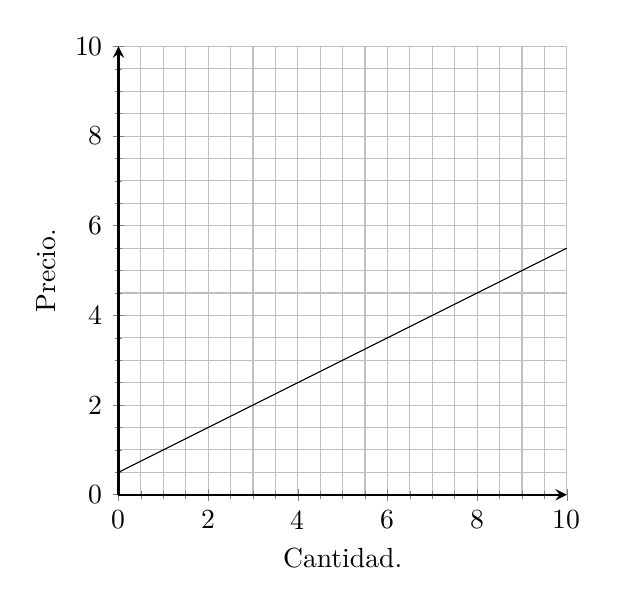
\begin{tikzpicture}
    \begin{axis}[grid=both,
    unit vector ratio*=1 1 1,
    axis x line=bottom,
    axis y line=left,
    axis line style=thick,
    xmax=10,xmin=0,
    ymax=10,ymin=0,
    xtick={0,2,4,6,8,10},
    ytick={0,2,4,6,8,10},
    minor tick num=3,
    xlabel=Cantidad.,
    ylabel=Precio.,
    ylabel near ticks,
    ylabel style={align=center},
    xlabel near ticks,
    ]
    
    \addplot[draw, smooth] coordinates {(0,0.5) (10,5.5)};
    \end{axis}
    \end{tikzpicture}
\end{center}
\end{multicols}

\hypertarget{demanda}{%
\section{Demanda:}\label{demanda}}

~ Mientras que la oferta se enfoca en el productor la demanda ve el
comportamiento de los consumidores. La cantidad demandada es cuanto está
dispuesto a comprar el consumidor para un determinado precio. La ley de
demanda dice que a mayor precio habrá una menor cantidad demandada.
Dicha relación, asumiendo una forma lineal se puede re-escribir como:

\[
P(Q)=a-bQ
\] ~ Para los valores \(a=21\), \(b=0.8\), que podría ser el mismo caso
anterior, el gráfico sería así:

\begin{multicols}{2}

\begin{table}[H]
    \centering
    \begin{tabular}{|p{25mm}|p{25mm}|}
        \multicolumn{2}{c}{Tabla de demanda:} \\
        \hline
        Precio: ($P$) & Cantidad ($Q$): \\ \hline
        20,2 & 1 \\ \hline
        19,4 & 2 \\ \hline
        18,6 & 3 \\ \hline
        17,8 & 4 \\ \hline
        17 & 5 \\ \hline
        16,2 & 6 \\ \hline
        15,4 & 7 \\ \hline
        14,6 & 8 \\ \hline
        13,8 & 9 \\ \hline
        \end{tabular}
\end{table}

\begin{center}
    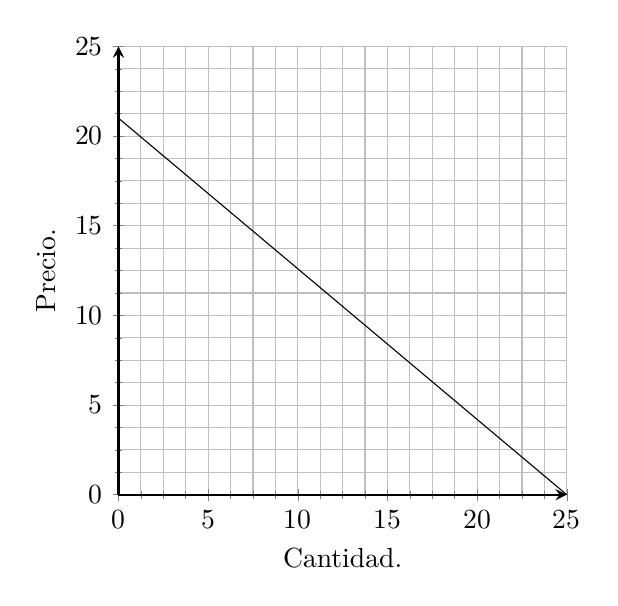
\begin{tikzpicture}
    \begin{axis}[grid=both,
    unit vector ratio*=1 1 1,
    axis x line=bottom,
    axis y line=left,
    axis line style=thick,
    xmax=25,xmin=0,
    ymax=25,ymin=0,
    xtick={0,5,10,15,20,25},
    ytick={0,5,10,15,20,25},
    minor tick num=3,
    xlabel=Cantidad.,
    ylabel=Precio.,
    ylabel near ticks,
    ylabel style={align=center},
    xlabel near ticks,
    ]
    
    \addplot[draw, smooth] coordinates {(0,21) (25,0)};
    \end{axis}
    \end{tikzpicture}
\end{center}

\end{multicols}

~ Como se puede ver, mientras más cantidad hay, menos demanda hay. Por
lo que el precio demandado baja.

\hypertarget{equilibrio-de-mercado}{%
\section{Equilibrio de mercado:}\label{equilibrio-de-mercado}}

~ Cuando el valor de la demanda y de la oferta son iguales, significa
que hay equilibrio de mercado. Esto se puede ver en la intersección de
ambas curvas en un gráfico.

~ Si decimos que los dos gráficos anteriores son del mismo bien entonces
el gráfico del equilibrio de mercado sería:

\begin{center}
    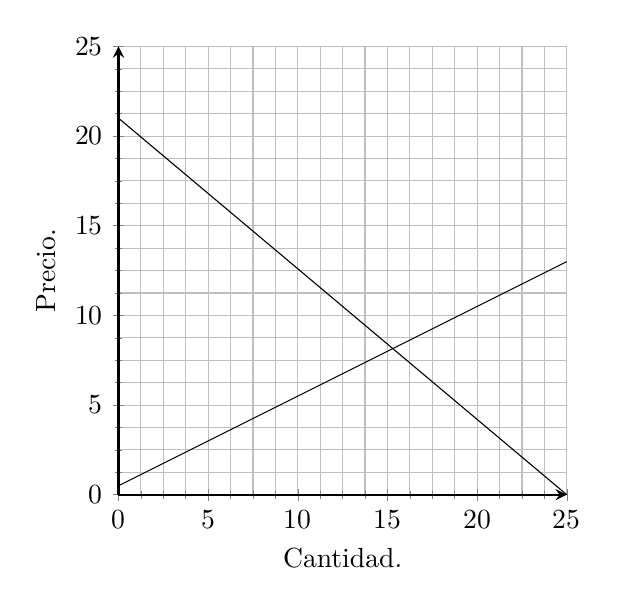
\begin{tikzpicture}
    \begin{axis}[grid=both,
    unit vector ratio*=1 1 1,
    axis x line=bottom,
    axis y line=left,
    axis line style=thick,
    xmax=25,xmin=0,
    ymax=25,ymin=0,
    xtick={0,5,10,15,20,25},
    ytick={0,5,10,15,20,25},
    minor tick num=3,
    xlabel=Cantidad.,
    ylabel=Precio.,
    ylabel near ticks,
    ylabel style={align=center},
    xlabel near ticks,
    ]
 
    \addplot[draw, smooth] coordinates {(0,21) (25,0)};
    \addplot[draw, smooth] coordinates {(0,0.5) (25,13)};
    \end{axis}
    \end{tikzpicture}
\end{center}

~ El punto de intersección es cuando el precio es de \$11 y hay 12.5
unidades de producción. Este es el punto de equilibrio de mercado, si el
mercado está sobre ese punto es que hay un exceso de oferta, y su está
más bajo, es que hay escasez.

\hypertarget{cambios-de-curvas}{%
\section{Cambios de curvas:}\label{cambios-de-curvas}}

~ Podemos analizar que sucediera si hay un cambio en la curva de oferta
y demanda, los cambios se relacionan de la siguiente forma:

\begin{table}[H]
    \centering
    \begin{tabular}{|p{25mm}|p{25mm}|p{25mm}|p{25mm}|p{25mm}|}
        \hline
         & Sin cambio en la oferta & Un incremento de la oferta & Un decremento de la oferta  \\ \hline
        Sin cambio en la oferta & P igual \par Q igual & P disminuye \par Q aumenta & P aumenta \par Q disminuye \\ \hline
        Un incremento de la oferta & P aumenta \par Q aumenta & P ambiguo \par Q aumenta & P aumenta \par Q ambiguo\\ \hline
        Un decremento de la oferta & P disminuye \par Q disminuye & P disminuye \par Q ambiguo & P ambiguo \par Q disminuye \\ \hline
    \end{tabular}
\end{table}

~ Por lo general, lo que hace que las curvas cambien de posición son
eventos bruscos, por ejemplo, en el mercado de las lecherías, si se
contamina con un antibiótico la central de ``colun'' la curva de oferta
aumentaría, ya que, es menos lo que se podría ofrecer.

~ Puede ocurrir que cambien las posiciones de ambas curvas
simultáneamente.

~ Ahora veremos cómo afecta esto en el punto de equilibrio:

~ Tomaremos como situación antes del cambio el siguiente gráfico.

\begin{center}
    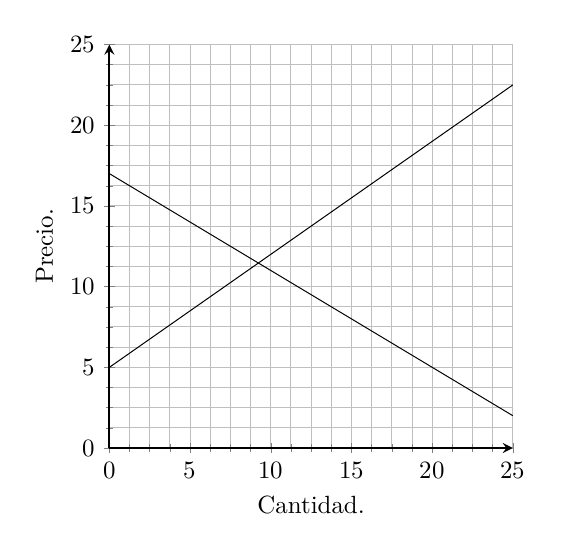
\begin{tikzpicture}[scale=0.9]
    \begin{axis}[grid=both,
    unit vector ratio*=1 1 1,
    axis x line=bottom,
    axis y line=left,
    axis line style=thick,
    xmax=25,xmin=0,
    ymax=25,ymin=0,
    xtick={0,5,10,15,20,25},
    ytick={0,5,10,15,20,25},
    minor tick num=3,
    xlabel=Cantidad.,
    ylabel=Precio.,
    ]
    \addplot [
    domain=0:25, 
    samples=100, 
    color=black,
    ]
    {5+0.7*x};
    \addplot [
    domain=0:25, 
    samples=100, 
    color=black,
    ]
    {17-0.6*x};
    \end{axis}
    \end{tikzpicture}
\end{center}

~ Los siguientes gráficos representan el cambio:

\begin{multicols}{2}
\begin{center}
    \indent Curva de oferta se desplaza hacia la izquierda:
    
    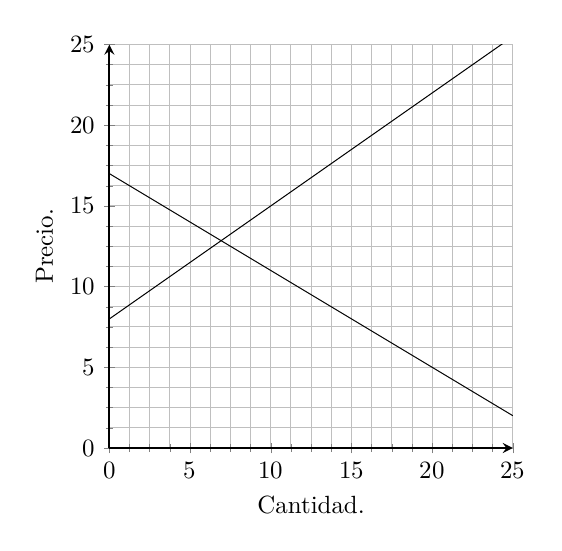
\begin{tikzpicture}[scale=0.9]
    \begin{axis}[grid=both,
    unit vector ratio*=1 1 1,
    axis x line=bottom,
    axis y line=left,
    axis line style=thick,
    xmax=25,xmin=0,
    ymax=25,ymin=0,
    xtick={0,5,10,15,20,25},
    ytick={0,5,10,15,20,25},
    minor tick num=3,
    xlabel=Cantidad.,
    ylabel=Precio.,
    ]
    \addplot [
    domain=0:25, 
    samples=100, 
    color=black,
    ]
    {8+0.7*x};
    \addplot [
    domain=0:25, 
    samples=100, 
    color=black,
    ]
    {17-0.6*x};
    \end{axis}
    \end{tikzpicture}
\end{center}

\begin{center}
    \indent Curva de demanda e desplaza hacia la derecha:
    
    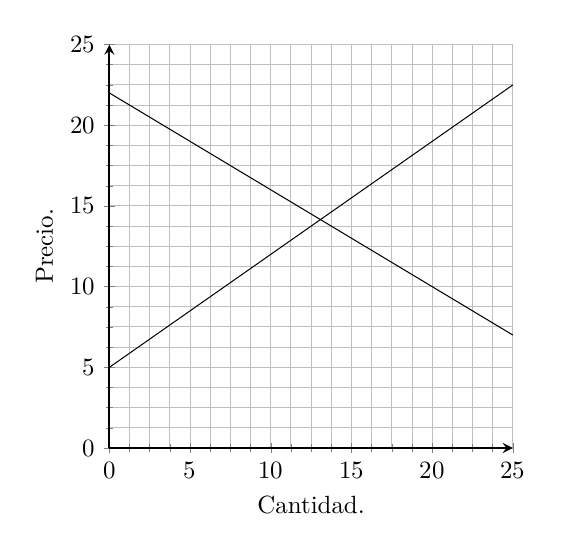
\begin{tikzpicture}[scale=0.9]
    \begin{axis}[grid=both,
    unit vector ratio*=1 1 1,
    axis x line=bottom,
    axis y line=left,
    axis line style=thick,
    xmax=25,xmin=0,
    ymax=25,ymin=0,
    xtick={0,5,10,15,20,25},
    ytick={0,5,10,15,20,25},
    minor tick num=3,
    xlabel=Cantidad.,
    ylabel=Precio.,
    ]
    \addplot [
    domain=0:25, 
    samples=100, 
    color=black,
    ]
    {5+0.7*x};
    \addplot [
    domain=0:25, 
    samples=100, 
    color=black,
    ]
    {22-0.6*x};
    \end{axis}
    \end{tikzpicture}
\end{center}

\end{multicols}

\newpage

\begin{multicols}{2}

\begin{center}
    \indent Curva de oferta e desplaza hacia la derecha:
    
    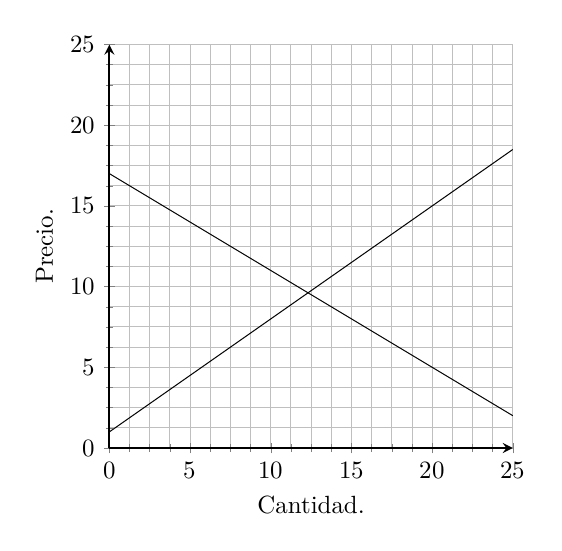
\begin{tikzpicture}[scale=0.9]
    \begin{axis}[grid=both,
    unit vector ratio*=1 1 1,
    axis x line=bottom,
    axis y line=left,
    axis line style=thick,
    xmax=25,xmin=0,
    ymax=25,ymin=0,
    xtick={0,5,10,15,20,25},
    ytick={0,5,10,15,20,25},
    minor tick num=3,
    xlabel=Cantidad.,
    ylabel=Precio.,
    ]
    \addplot [
    domain=0:25, 
    samples=100, 
    color=black,
    ]
    {1+0.7*x};
    \addplot [
    domain=0:25, 
    samples=100, 
    color=black,
    ]
    {17-0.6*x};
    \end{axis}
    \end{tikzpicture}
\end{center}
 
\begin{center}
    \indent Curva de demanda e desplaza hacia la izquierda:
    
    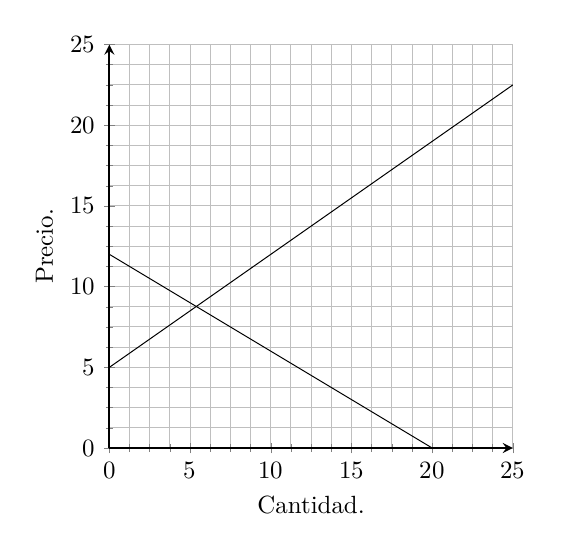
\begin{tikzpicture}[scale=0.9]
    \begin{axis}[grid=both,
    unit vector ratio*=1 1 1,
    axis x line=bottom,
    axis y line=left,
    axis line style=thick,
    xmax=25,xmin=0,
    ymax=25,ymin=0,
    xtick={0,5,10,15,20,25},
    ytick={0,5,10,15,20,25},
    minor tick num=3,
    xlabel=Cantidad.,
    ylabel=Precio.,
    ]
    \addplot [
    domain=0:25, 
    samples=100, 
    color=black,
    ]
    {5+0.7*x};
    \addplot [
    domain=0:25, 
    samples=100, 
    color=black,
    ]
    {12-0.6*x};
    \end{axis}
    \end{tikzpicture}
\end{center}

\end{multicols}

\hypertarget{elasticidad}{%
\section{Elasticidad:}\label{elasticidad}}

~ La elasticidad es una medida que refleja la capacidad de respuesta de
la cantidad demandada u ofrecida ante variaciones en el precio.

~ Primero, se definirá la elasticidad de la demanda. Esta se relaciona
con la cantidad demandada, manteniendo constantes factores como ingreso,
preferencias y otras variables. La elasticidad de la cantidad demandada
ante variaciones en el precio se determina por cuánto cambia la cantidad
demandada cuando hay un cambio en el precio. Se utilizarán variaciones
porcentuales para calcular la elasticidad, lo cual puede ser un poco
complicado debido a la pendiente constante en una función lineal.

~ La elasticidad puede calcularse respecto a cualquier factor en la
función de demanda o de oferta. En la oferta, se analizan costos y el
costo marginal, que influye en las cantidades ofrecidas en el mercado.

~ Un ejemplo típico de elasticidad es la elasticidad precio, que mide
cómo cambia la cantidad demandada cuando cambia el precio de este bien.
Esta medida es útil para empresas al tomar decisiones sobre precios, ya
que permite anticipar cómo reaccionarán los consumidores a cambios en el
precio. Si se baja el precio y la cantidad demandada no aumenta, puede
haber un problema con la ley de demanda, indicando que otros
determinantes están influyendo.

~ En la práctica, la elasticidad también se utiliza para evaluar el
impacto de cambios en precios de bienes complementarios o sustitutos.
Por ejemplo, un aumento en el precio de un bien complementario reducirá
la cantidad demandada del bien en análisis, mientras que un aumento en
el precio de un bien sustituto puede aumentar la demanda del bien en
análisis.

~ La elasticidad de la oferta también sigue principios similares,
evaluando cómo varía la cantidad ofrecida ante cambios en el precio. Un
análisis completo de elasticidad implica entender estos conceptos tanto
para la demanda como para la oferta, y cómo se reflejan en el mercado.

~ En el análisis de la elasticidad, se destaca cómo una demanda puede
ser perfectamente inelástica o elástica, y los extremos intermedios. Una
demanda perfectamente inelástica no cambia la cantidad demandada ante
variaciones en el precio, mientras que una demanda perfectamente
elástica cambia drásticamente la cantidad demandada ante pequeñas
variaciones en el precio.

~ La elasticidad nos ayuda a entender mejor la asignación de recursos en
mercados competitivos y las estrategias de precios que pueden adoptarse
para optimizar ingresos y satisfacer la demanda.

~ La elasticidad mide cómo la cantidad demandada u ofrecida responde a
cambios en el precio. En mercados con alta elasticidad, pequeños cambios
en el precio pueden llevar a grandes cambios en la cantidad demandada u
ofrecida. En mercados con baja elasticidad, los cambios en el precio
tienen un efecto menor.

~ La elasticidad de la oferta y la demanda se calcula con esta fórmula:
\[
\in =\left|\frac{\triangle\%Q}{\triangle\%P} \right|
\] ~ Donde \(\in\) es la elasticidad, \(\triangle\%\) el cambio
porcentual, Q es la demanda y P el precio.

\[
f(x)= \left\{ \begin{array}{lcc}
     \text{Inelástica} &   \text{si}  & \in < 1 \\
     \\ \text{Absolutamente inelástica} &  \text{si} & \in = 0 \\
     \\ \text{Elasticidad unitaria} &  \text{si}  & \in = 1 \\
     \\ \text{Elástica} &  \text{si}  & \in > 1
     \end{array}
\right.
\]

~ \ul{Ejercicio resuelto:}

~ Tenemos las siguientes expresiones \(P_1(Q)\) y \(P_2(Q)\) que son la
ecuación de oferta hace un año y de ahora respectivamente y \(P_3(Q)\) y
\(P_4(Q)\) que son la ecuación de demanda de hace un año y actual,
calcule y clasifique su elasticidad.

\[
\begin{matrix}
    P_1(Q)=10+4Q &  P_2(Q)=30+4Q \\
    P_3(Q)=310-6Q & P_4(Q)=200-6Q \\
\end{matrix}
\]

~ \textbf{Respuesta:}

~ \ul{Paso I: encontrar el equilibrio de mercado del antes y el ahora.}

~ Equilibrio antiguo:

\[
10+4Q=310-6Q \Leftrightarrow 300=10Q \Leftrightarrow Q=30
\]

\[
P_3(Q)=310-6 \cdot 30 \Leftrightarrow P_3 = P_1 = 130
\]

\[
(30,130)
\]

~ Equilibrio actual:

\[
30+4Q=200-6Q \Leftrightarrow 170=10Q \Leftrightarrow Q=17
\]

\[
P_2(Q)=30+4 \cdot 17 \Leftrightarrow P_2 = P_4 = 98
\]

\[
(17,98)
\]

~ \ul{Paso II: Calcular la elasticidad y clasificarla.}

\[
\in =\left|\dfrac{1-\frac{17}{30}}{1-\frac{98}{130}} \right|
\]

\[
\in =\dfrac{\frac{13}{30}}{\frac{32}{130}}
\]

\[
\in =\dfrac{1690}{960}
\]

\[
\in =1,7604
\]

~ Es elástica.

\bookmarksetup{startatroot}

\hypertarget{intervenciones-del-mercado.}{%
\chapter{Intervenciones del
mercado.}\label{intervenciones-del-mercado.}}

\hypertarget{economuxeda-de-bienestar}{%
\section{Economía de bienestar:}\label{economuxeda-de-bienestar}}

~ La economía de bien estar se basa en la disposición de un comprador a
pagar o un productor a producir. Por lo que se puede ver desde el punto
de vista del oferente y del demandante:

~ En el siguiente gráfico veremos de forma clara la representación de
ambos puntos de vista:

\begin{figure}

{\centering \includegraphics[width=0.6\textwidth,height=\textheight]{3interverción_files/figure-pdf/unnamed-chunk-1-1.pdf}

}

\end{figure}

~ Donde
\texttt{EC\textquotesingle{}\textquotesingle{}\ es\ el\ excedente\ del\ consumidor\ y}EP'\,'
es el excedente del productor.

~ \textbf{Excedente del consumidor:}

~ Se calcula como el precio que está dispuesto a pagar el consumidor
menos lo que paga. De forma puntual se puede formular como: \[
ec = p_c - P_e
\]

~ Donde \(ec\) es el excedente de un consumidor especifico, \(p_c\) es
el precio máximo dispuesto a pagar y \(P_e\) el precio en el equilibrio.

~ De forma general es el área marcada con naranjo en el gráfico, pero
también lo puedes calcular con la siguiente formula. \[
EC = \int_{0}^{Q_e}{P_d(Q)-P_e \ dQ}
\]

~ Donde ``\(P_e\)'' es el precio de equilibrio y ``\(Q_0\)'', es la
cantidad en el equilibrio.

~ \textbf{Excedente del productor:}

~ De forma general es el área marcada con naranjo en el gráfico, pero
también lo puedes calcular con la siguiente formula. \[
EC = \int_{0}^{Q_e}{P_e-P_s(Q) \ dQ}
\]

\hypertarget{intervenciuxf3n-del-gobierno}{%
\section{Intervención del
gobierno:}\label{intervenciuxf3n-del-gobierno}}

~ La intervención gubernamental, es un tema central en la economía
pública y del sector público. La intervención del gobierno puede
justificarse por diversas razones, como corregir fallas del mercado,
redistribuir ingresos o mejorar la eficiencia económica.

~ Las intervenciones estatales son cambios forzados que hace el gobierno
a un mercado, estos generan una pérdida de eficiencia, también llamada
\textbf{peso muerto}, esto hace que cambien las decisiones de las
personas.

~ Una de las formas de intervención del gobierno es agregar por ley un
\textbf{precio máximo}, este es el precio máximo legal, y también puede
agregar un \textbf{precio mínimo} que es el precio mínimo legal. Si el
precio máximo esta por sobre el equilibrio no influye en el mercado,
pero si esta por debajo, genera escasez. Por otro lado, si el precio
mínimo esta por debajo del equilibrio, no influye en el mercado. Por el
contrario, si esta sobre el equilibrio genera superávit.

~ Para que el gobierno se financie, les agrega un impuesto a los
productos que hará subir el costo y precio de estos, dicho de otra forma
el excedente del consumidor y productor disminuye, y ambos pagan la
misma cantidad de impuesto al comprar o vender ese producto.

~ También existen otras intervenciones del estado, como, por ejemplo, el
subsidio, se le conoce como el impuesto negativo, ya que, el consumidor
paga menos. Igual que los impuestos, pero de forma contraría, la
financiación del estado es repartido equitativamente entre los
participantes de ese mercado.

~ La intervención gubernamental, es un tema central en la economía
pública y del sector público. La intervención del gobierno puede
justificarse por diversas razones, como corregir fallas del mercado,
redistribuir ingresos o mejorar la eficiencia económica.

~ Los siguientes gráficos son posibles ejemplos de ambas situaciones.
Donde,
\texttt{O\ mer\textquotesingle{}\textquotesingle{}\ es\ oferta\ sin\ impuesto\ o\ subsidio,}D
mer'\,' es demanda sin impuesto o subsidio, el área negra es la perdida
de eficiencia o peso muerto, ``GOB'\,' es lo que recibe o financia el
gobierno, dependiendo si es impuesto o subsidio respectivamente y EC y
EP son los excedentes del consumidor y productor respectivamente.

~ \textbf{Impuestos:} Dependiendo de si los impuestos son impuestos a
los vendedores o a los compradores, sus efectos pueden variar. Un
impuesto sobre los vendedores puede contraer la oferta, ya que estos
deben pagar una parte de sus ingresos al gobierno, lo que puede reducir
su incentivo para producir. Por otro lado, un impuesto sobre los
compradores puede reducir la demanda, ya que el bien se vuelve más caro
para los consumidores.

\begin{multicols}{2}

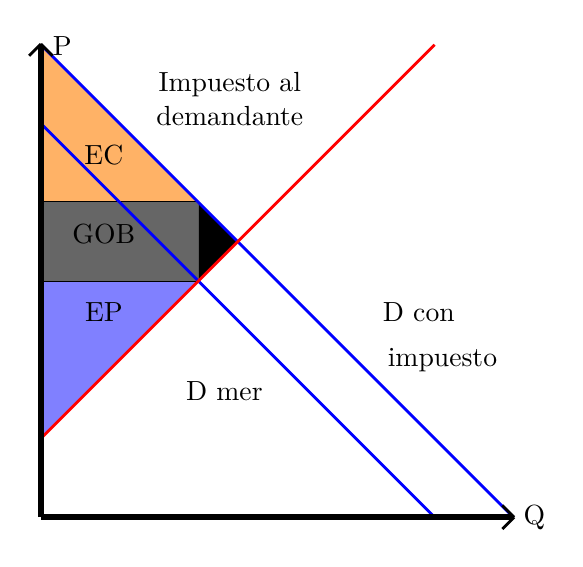
\begin{tikzpicture}

    % oferta = P(Q)=1+Q
    % demanda libre = P(Q)=5-Q
    % demanda con impuesto = 6-Q
    
    
    % Etiquetas en el eje P
    % Area excedente del consumidor
    \fill[orange!60] (0,4) -- (2,4) -- (0,6) -- cycle;
    \draw [line width=1pt](0,4) -- (2,4);
    
    % Area excedente del productor
    \fill[blue!50] (0,3) -- (2,3) -- (0,1) -- cycle;
    \draw [line width=1pt](0,3) -- (2,3);
    
    % Area de impuesto recuadado.
    \fill[black!60] (0,4) -- (2,4) -- (2,3) -- (0,3)-- cycle;
    
    % perdida de eficiencia.
    \fill[black] (2,3) -- (2,4) -- (2.5,3.5) -- cycle;
    
    % demanda sin impuesto
    \draw [blue, line width=1pt](0,5) -- (5,0); %P(Q)=5-Q

    %demanda con impuesto
    \draw [blue, line width=1pt](0,6) -- (6,0);

    % oferta
    \draw [red, line width=1pt](0,1) -- (5,6); %P(Q)=1+Q
       
    % Eje x
    \draw[black, line width=2pt] (0,0) -- (5.98,0) node[right] {Q};
    \draw[black, line width=1pt] (5.86,-0.15) -- (6.01,0);
    \draw[black, line width=1pt] (5.86,0.15) -- (6.01,0);

    % eje y
    \draw[black, line width=2pt] (0,0) -- (0,5.98) node[right] {P};
    \draw[black, line width=1pt] (-0.15,5.86) -- (0,6.01);
    \draw[black, line width=1pt] (0.15,5.86) -- (0,6.01);

    %leyendas
    \node at (0.8,2.6) {EP};
    \node at (0.8,4.6) {EC};
    \node at (0.8,3.6) {GOB};
    \node at (4.8,2.6) {D con};
    \node at (5.1,2) {impuesto};
    \node at (2.33,1.6) {D mer};
    \node at (2.4,5.5) {Impuesto al};
    \node at (2.4,5.1) {demandante};
    
\end{tikzpicture}

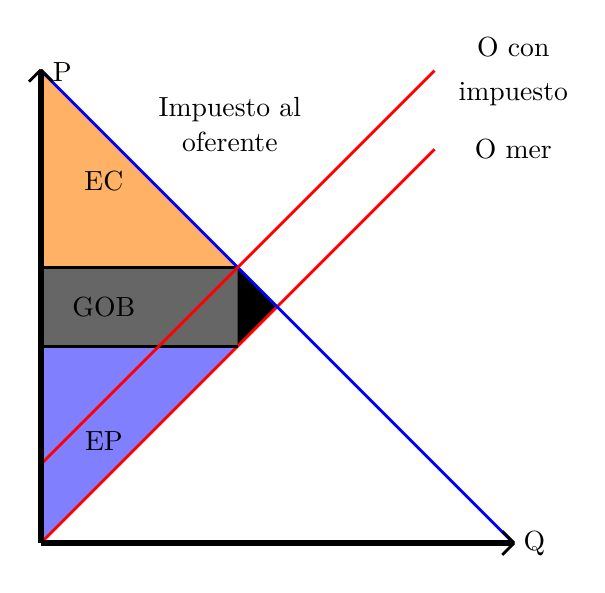
\begin{tikzpicture}

    % oferta = P(Q)=1+Q
    % demanda libre = P(Q)=5-Q
    % demanda con impuesto = 6-Q
    
    
    % Etiquetas en el eje P
    % Area excedente del consumidor
    \fill[orange!60] (0,3.5) -- (2.5,3.5) -- (0,6) -- cycle;
    
    % Area excedente del productor
    \fill[blue!50] (0,2.5) -- (2.5,2.5) -- (0,0) -- cycle;
    
    % Area de impuesto recuadado.
    \fill[black!60] (0,2.5) -- (0,3.5) -- (2.5,3.5) -- (2.5,2.5)-- cycle;
    
    % perdida de eficiencia.
    \fill[black] (2.5,3.5) -- (2.5,2.5) -- (3,3) -- cycle;
    
    % oferta sin impuesto
    \draw [red, line width=1pt](0,0) -- (5,5); %P(Q)=5-Q
    \draw [line width=1pt](0,2.5) -- (2.5,2.5);
    \draw [line width=1pt](0,3.5) -- (2.5,3.5);

    %demanda con impuesto
    \draw [blue, line width=1pt](0,6) -- (6,0);

    % oferta
    \draw [red, line width=1pt](0,1) -- (5,6); %P(Q)=1+Q
    
    % Eje x
    \draw[black, line width=2pt] (0,0) -- (5.98,0) node[right] {Q};
    \draw[black, line width=1pt] (5.86,-0.15) -- (6.01,0);
    \draw[black, line width=1pt] (5.86,0.15) -- (6.01,0);

    % eje y
    \draw[black, line width=2pt] (0,0) -- (0,5.98) node[right] {P};
    \draw[black, line width=1pt] (-0.15,5.86) -- (0,6.01);
    \draw[black, line width=1pt] (0.15,5.86) -- (0,6.01);

    %leyendas
    \node at (0.8,1.3) {EP};
    \node at (0.8,4.6) {EC};
    \node at (0.8,3) {GOB};
    \node at (6,6.3) {O con};
    \node at (6,5.7) {impuesto};
    \node at (6,5) {O mer};
    \node at (2.4,5.5) {Impuesto al};
    \node at (2.4,5.1) {oferente};
    
\end{tikzpicture}

\end{multicols}

~ \textbf{Subsidios:} Los subsidios pueden ser utilizados para
incentivar tanto la producción como el consumo. Un subsidio a los
productores reduce sus costos de producción, lo que puede aumentar la
oferta. Un subsidio a los consumidores reduce el precio efectivo que
pagan, aumentando la demanda. Sin embargo, los subsidios también deben
ser cuidadosamente diseñados para evitar distorsiones excesivas en el
mercado.

\begin{multicols}{2}

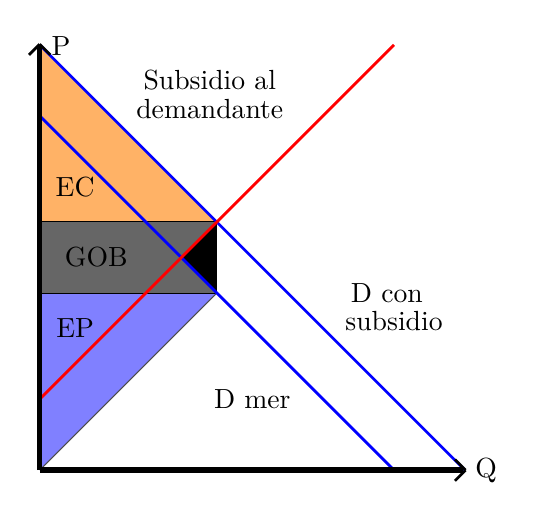
\begin{tikzpicture}[scale=0.9]

    % oferta = P(Q)=1+Q
    % demanda libre = P(Q)=5-Q
    % demanda con subsidio = 4-Q
    
    
    % Etiquetas en el eje P
    % Area excedente del consumidor
    \fill[orange!60] (0,3.5) -- (2.5,3.5) -- (0,6) -- cycle;
    \draw [line width=1pt](0,3.5) -- (2.5,3.5);
    
    % Area excedente del productor
    \fill[blue!50] (0,2.5) -- (2.5,2.5) -- (0,0) -- cycle;
    \draw [line width=1pt](0,2.5) -- (2.5,2.5);
    \draw [black!70](0,0) -- (2.5,2.5);
    
    % Area de impuesto recuadado.
    \fill[black!60] (0,2.5) -- (0,3.5) -- (2.5,3.5) -- (2.5,2.5)-- cycle;
    
    % perdida de eficiencia.
    \fill[black] (2,3) -- (2.5,2.5) -- (2.5,3.5) -- cycle;
    
    % demanda sin subsidio
    \draw [blue, line width=1pt](0,5) -- (5,0); %P(Q)=5-Q

    %demanda con subsidio
    \draw [blue, line width=1pt](0,6) -- (6,0);

    % oferta
    \draw [red, line width=1pt](0,1) -- (5,6); %P(Q)=1+Q
    
    % Eje x
    \draw[black, line width=2pt] (0,0) -- (5.98,0) node[right] {Q};
    \draw[black, line width=1pt] (5.86,-0.15) -- (6.01,0);
    \draw[black, line width=1pt] (5.86,0.15) -- (6.01,0);

    % eje y
    \draw[black, line width=2pt] (0,0) -- (0,5.98) node[right] {P};
    \draw[black, line width=1pt] (-0.15,5.86) -- (0,6.01);
    \draw[black, line width=1pt] (0.15,5.86) -- (0,6.01);

    %leyendas
    \node at (0.5,2) {EP};
    \node at (0.5,4) {EC};
    \node at (0.8,3) {GOB};
    \node at (4.9,2.5) {D con};
    \node at (5,2.1) {subsidio};
    \node at (3,1) {D mer};
    \node at (2.4,5.5) {Subsidio al};
    \node at (2.4,5.1) {demandante};
    
\end{tikzpicture}

\columnbreak

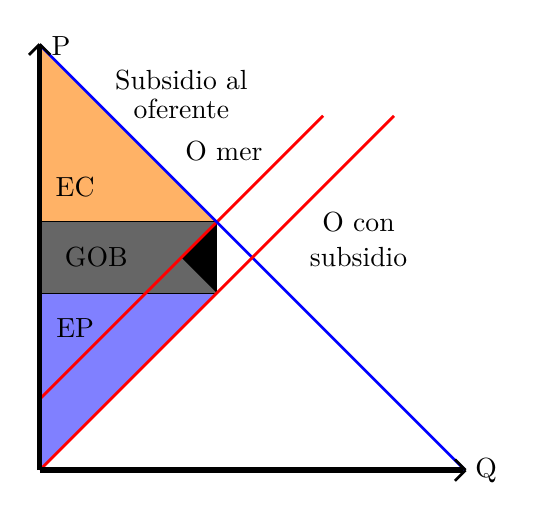
\begin{tikzpicture}[scale=0.9]

    % oferta = P(Q)=1+Q
    % demanda libre = P(Q)=5-Q
    % demanda con subsidio = 4-Q
    
    
    % Etiquetas en el eje P
    % Area excedente del consumidor
    \fill[orange!60] (0,3.5) -- (2.5,3.5) -- (0,6) -- cycle;
    \draw [line width=1pt](0,3.5) -- (2.5,3.5);
    
    % Area excedente del productor
    \fill[blue!50] (0,2.5) -- (2.5,2.5) -- (0,0) -- cycle;
    \draw [line width=1pt](0,2.5) -- (2.5,2.5);
    
    % Area de subsidio recuadado.
    \fill[black!60] (0,2.5) -- (0,3.5) -- (2.5,3.5) -- (2.5,2.5)-- cycle;
    
    % perdida de eficiencia.
    \fill[black] (2.5,2.5) -- (2.5,3.5) -- (2,3) -- cycle;
    
    % oferta sin subsidio
    \draw [red, line width=1pt](0,1) -- (4,5); %P(Q)=5-Q

    %demanda
    \draw [blue, line width=1pt](0,6) -- (6,0);

    % oferta
    \draw [red, line width=1pt](0,0) -- (5,5); %P(Q)=1+Q
    
    % Eje x
    \draw[black, line width=2pt] (0,0) -- (5.98,0) node[right] {Q};
    \draw[black, line width=1pt] (5.86,-0.15) -- (6.01,0);
    \draw[black, line width=1pt] (5.86,0.15) -- (6.01,0);

    % eje y
    \draw[black, line width=2pt] (0,0) -- (0,5.98) node[right] {P};
    \draw[black, line width=1pt] (-0.15,5.86) -- (0,6.01);
    \draw[black, line width=1pt] (0.15,5.86) -- (0,6.01);

    %leyendas
    \node at (0.5,2) {EP};
    \node at (0.5,4) {EC};
    \node at (0.8,3) {GOB};
    \node at (2.6,4.5) {O mer};
    \node at (4.5,3.5) {O con};
    \node at (4.5,3) {subsidio};
    \node at (2,5.5) {Subsidio al};
    \node at (2,5.1) {oferente};
    
\end{tikzpicture}

\end{multicols}

~ \textbf{Controles de Precios:}

\begin{itemize}
\item
  \textbf{Precios Máximos:} Un precio máximo establecido por debajo del
  precio de equilibrio del mercado puede causar escasez. Esto ocurre
  porque a un precio más bajo, la cantidad demandada aumenta mientras
  que la cantidad ofrecida disminuye. Los consumidores encuentran el
  bien más accesible, incrementando su demanda, pero los productores no
  están dispuestos a vender tanto debido al menor incentivo económico,
  lo que reduce la oferta.
\item
  \textbf{Precios Mínimos:} Un precio mínimo por encima del precio de
  equilibrio del mercado genera un exceso de oferta. A este precio más
  alto, los productores están dispuestos a ofrecer más del bien o
  servicio, pero los consumidores no están dispuestos a comprar tanto,
  reduciendo la cantidad demandada.
\end{itemize}

\begin{multicols}{2}

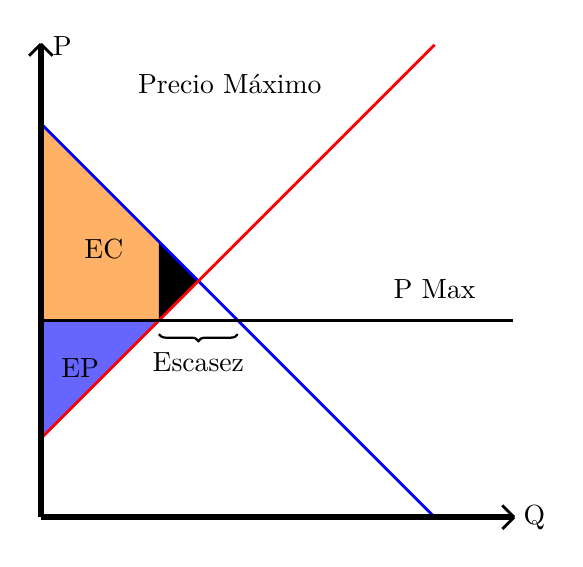
\begin{tikzpicture}

    % oferta = P(Q)=1+Q
    % demanda = P(Q)=5-Q
    
    
    % Etiquetas en el eje P
    % Area excedente del consumidor
    \fill[orange!60] (0,2.5) -- (0,5) -- (1.5,3.5) -- (1.5,2.5) -- cycle;
    
    % Area excedente del productor
    \fill[blue!60] (0,2.5) -- (1.5,2.5) -- (0,1) -- cycle;
    
    % perdida de eficiencia.
    \fill[black] (2,3) -- (1.5,3.5) -- (1.5,2.5) -- cycle;
    
    % demanda
    \draw [blue, line width=1pt](0,5) -- (5,0); %P(Q)=5-Q

    % oferta
    \draw [red, line width=1pt](0,1) -- (5,6); %P(Q)=1+Q
    
    \draw [line width=1pt](0,2.5) -- (6,2.5);
    
    % Eje x
    \draw[black, line width=2pt] (0,0) -- (5.98,0) node[right] {Q};
    \draw[black, line width=1pt] (5.86,-0.15) -- (6.01,0);
    \draw[black, line width=1pt] (5.86,0.15) -- (6.01,0);

    % eje y
    \draw[black, line width=2pt] (0,0) -- (0,5.98) node[right] {P};
    \draw[black, line width=1pt] (-0.15,5.86) -- (0,6.01);
    \draw[black, line width=1pt] (0.15,5.86) -- (0,6.01);

    %leyendas
    \node at (0.5,1.9) {EP};
    \node at (0.8,3.4) {EC};
    \draw [thick, decoration={brace, mirror, raise=5pt}, decorate] (1.5,2.5) -- (2.5,2.5) node[midway, below=8pt] {Escasez};
    \node at (5,2.9) {P Max};
    \node at (2.4,5.5) {Precio Máximo};
\end{tikzpicture}

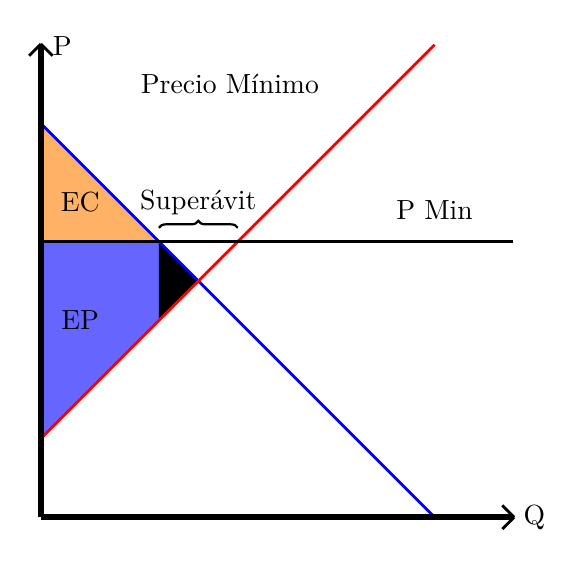
\begin{tikzpicture}

    % oferta = P(Q)=1+Q
    % demanda = P(Q)=5-Q
    
    
    % Etiquetas en el eje P
    % Area excedente del consumidor
    \fill[orange!60] (0,3.5) -- (0,5) -- (1.5,3.5) -- cycle;
    
    % Area excedente del productor
    \fill[blue!60] (0,1) -- (0,3.5) -- (1.5,3.5) -- (1.5,2.5) -- cycle;
    
    % perdida de eficiencia.
    \fill[black] (2,3) -- (1.5,3.5) -- (1.5,2.5) -- cycle;
    
    % demanda
    \draw [blue, line width=1pt](0,5) -- (5,0); %P(Q)=5-Q

    % oferta
    \draw [red, line width=1pt](0,1) -- (5,6); %P(Q)=1+Q
    
    \draw [line width=1pt](0,3.5) -- (6,3.5);
    
    % Eje x
    \draw[black, line width=2pt] (0,0) -- (5.98,0) node[right] {Q};
    \draw[black, line width=1pt] (5.86,-0.15) -- (6.01,0);
    \draw[black, line width=1pt] (5.86,0.15) -- (6.01,0);

    % eje y
    \draw[black, line width=2pt] (0,0) -- (0,5.98) node[right] {P};
    \draw[black, line width=1pt] (-0.15,5.86) -- (0,6.01);
    \draw[black, line width=1pt] (0.15,5.86) -- (0,6.01);

    %leyendas
    \node at (0.5,2.5) {EP};
    \node at (0.5,4) {EC};
    \draw [thick, decoration={brace, raise=5pt}, decorate] (1.5,3.5) -- (2.5,3.5);
    \node at (5,3.9) {P Min};
    \node at (2,4) {Superávit};
    \node at (2.4,5.5) {Precio Mínimo};
    
\end{tikzpicture}

\end{multicols}

~ \textbf{Ejemplos Prácticos:}

\begin{itemize}
\item
  \textbf{Mercados de Alquiler:} En ciudades con altos precios de
  alquiler, un control de precios puede mejorar la accesibilidad, pero
  también puede reducir la oferta de viviendas si los propietarios no
  encuentran rentable alquilar a precios controlados.
\item
  \textbf{Mercado Laboral:} El ejemplo del salario mínimo mostró cómo la
  intervención en el mercado laboral puede tener efectos mixtos.
  Mientras que un salario mínimo más alto puede aumentar los ingresos de
  los trabajadores, también puede reducir las oportunidades de empleo.
\item
  \textbf{Impuestos al Tabaco:} Un impuesto al tabaco puede reducir el
  consumo debido al aumento del precio, lo que puede ser deseable desde
  una perspectiva de salud pública. Sin embargo, este impuesto también
  puede tener efectos regresivos si afecta desproporcionadamente a los
  consumidores de bajos ingresos.
\end{itemize}

\hypertarget{comercio-internacional}{%
\section{Comercio internacional:}\label{comercio-internacional}}

~ Existe un término que se llama \textbf{precio mundial} que hace
referencia al valor del costo de oportunidad. Esto hace que exista una
ventaja comparativa en cada país que incentiva a cada país a
especializarse en algún o algunos bienes específicos.

~ Para saber si conviene importar o exportar se hace un diagrama
agregando el precio mundial y el excedente al exportar o importar un
bien.

~ \textbf{Exportaciones.}

~ En el caso de una economía local, que tenga un precio en el equilibrio
menor que el del precio mundial y decida exportar, tendrá un gráfico,
donde
\texttt{BE\textquotesingle{}\textquotesingle{}\ es\ el\ beneficio\ de\ exportación\ y}PM'\,'
es el precio mundial, de la siguiente manera:

\begin{figure}

{\centering \includegraphics[width=0.5\textwidth,height=\textheight]{3interverción_files/figure-pdf/unnamed-chunk-8-1.pdf}

}

\end{figure}

~ \textbf{Importaciones.}

~ Para el caso de las importaciones sucede porque el precio de
equilibrio local es más alto que el precio mundial. Entonces, los
consumidores deciden importar. En este caso, llamaremos a ``BI'' como lo
que no se pierde por la decisión de importar.

\newpage

\begin{figure}

{\centering \includegraphics[width=0.5\textwidth,height=\textheight]{3interverción_files/figure-pdf/unnamed-chunk-9-1.pdf}

}

\end{figure}

~ \textbf{Arancel:}

~ El \textbf{arancel} por su parte es un impuesto a los productos
traídos del extranjero creando que el precio de estos suba. Esto influye
en los consumidores del país, porque el valor de lo que compren va a ser
igual a la suma del arancel y el precio mundial. En el gráfico ``Ar'' lo
llamaremos arancel, el área negra será la perdida de eficiencia y
``PA'', lo que gana el gobierno por medio del arancel.

\begin{figure}

{\centering \includegraphics[width=0.5\textwidth,height=\textheight]{3interverción_files/figure-pdf/unnamed-chunk-10-1.pdf}

}

\end{figure}

\hypertarget{consecuencias-de-la-intervenciuxf3n-en-los-participantes-de-un-mercado.}{%
\section{Consecuencias de la intervención en los participantes de un
mercado.}\label{consecuencias-de-la-intervenciuxf3n-en-los-participantes-de-un-mercado.}}

~ Como vimos en los gráficos anteriores al hacer una intervención en el
mercado, algunos participantes pueden ganar o perder excedente. Aun así,
es importante aclarar que un mercado intervenido, siempre tendrá su
dosis de ineficiencia. En las siguientes tablas veremos como afecta en
cada tipo de intervención.

\begin{table}[H]
    \centering
    \begin{tabular}{|p{45mm}|p{30mm}|p{30mm}|}
        \hline
        Intervención & Demandante & Oferente \\
        \hline
        Impuesto & Pierde excedente & Pierde excedente \\
        \hline
        Subsidio & Gana excedente & Gana excedente \\
        \hline
        Fijación precio máximo & Pierde excedente & Gana excedente \\
        \hline
        Fijación precio mínimo & Gana excedente & Pierde excedente \\
        \hline
    \end{tabular}
    \caption{Intervención I.}
    
\end{table}

~ Para el caso del comercio internacional sería de la siguiente forma:

\begin{table}[H]
    \centering
    \begin{tabular}{|p{48mm}|p{30mm}|p{30mm}|p{30mm}|}
        \hline
        Intervención & Productor local & Productor internacional. & Demandante local \\
        \hline
        Aplicar arancel o cerrarse al mercado internacional. & Gana excedente & Pierde excedente en dicho lugar & Pierde excedente \\
        \hline
        Eliminar arancel o abrirse al mercado internacional. & Pierde excedente & Gana excedente en dicho lugar & Gana excedente \\
        \hline
    \end{tabular}
    \caption{Intervención II.}
    
\end{table}

\bookmarksetup{startatroot}

\hypertarget{sistema-impositivo-y-economuxeda-laboral.}{%
\chapter{Sistema impositivo y economía
laboral.}\label{sistema-impositivo-y-economuxeda-laboral.}}

\hypertarget{financiamiento-del-gobierno}{%
\section{Financiamiento del
gobierno:}\label{financiamiento-del-gobierno}}

~ El gobierno necesita financiar sus gastos, para esto tiene dos
maneras, usar el impuesto o la deuda.

~ Si el gobierno gasta más de lo que recibe, entonces tiene un
\textbf{déficit presupuestario}, pero si gasta menos de lo que recibe
tiene un \textbf{superávit presupuestal}.

~ Los impuestos dan principalmente cargos administrativos para que la
gente cumpla las leyes fiscales.

~ Un sistema impositivo es más eficiente mientras recauda más ingreso y
mientras menos sea el costo de los contribuyentes, es decir,
equitativamente.

~ En el principio de beneficios dice que todos deben pagar sus impuestos
con respecto a los beneficios que recibe del gobierno. Mientras que el
principio de pago dice que los impuestos deben ser cobrados según dos
tipos de equidad, \textbf{Equidad horizontal:} los contribuyentes con
misma capacidad de pago pagan igual cantidad y \textbf{Equidad
vertical:} los contribuyentes con mayor capacidad de pago pagan más.

~ Los impuestos pueden ser: \textbf{proporcionales}, es decir, todos
deben pagar la misma fracción de sus ingresos, \textbf{regresivos}, los
contribuyentes con mayor ingreso deben pagar una fracción menor de su
ingreso que los con menor ingreso o \textbf{progresivos}, los
contribuyentes con menor ingreso deben pagar una fracción menor de su
ingreso que los con mayor ingreso.

~ El impuesto altera el equilibrio de precios, por lo que muchas veces
no se toma en cuenta en la decisión de estos las consecuencias
indirectas.

\hypertarget{fallas-del-mercado}{%
\section{Fallas del mercado:}\label{fallas-del-mercado}}

~ Las fallas de mercado como situaciones en las cuales los mercados no
logran alcanzar una solución eficiente. Estas fallas pueden surgir por
diversas razones, como la existencia de externalidades, bienes públicos,
información asimétrica, y monopolios naturales. Cada una de estas fallas
presenta desafíos únicos que pueden justificar la intervención del
gobierno.

~ La economía de bienestar tiene una fuga al no tomar dos supuestos
importantes:

\begin{enumerate}
\def\labelenumi{\arabic{enumi}.}
\item
  \textbf{Poder de mercado:} Hay veces que existe un solo vendedor
  (monopolio) o un solo vendedor (monopsonio).
\item
  \textbf{externalidades:} Las decisiones de los compradores y
  vendedores a veces afectan a algún tercero y no paga o compensa el
  daño a este último, un ejemplo típico es la contaminación.
\end{enumerate}

~ Una externalidad ocurre cuando la acción de una persona afecta el
bienestar de otra sin que exista una compensación por dicho efecto. Las
externalidades pueden ser positivas o negativas.

\begin{itemize}
\item
  \textbf{Externalidades Negativas:} Un ejemplo clásico es la
  contaminación. La producción de bienes en una fábrica puede liberar
  contaminantes al aire o al agua, afectando negativamente la salud de
  las personas y el medio ambiente. Este costo no se refleja en el
  precio del producto, lo que lleva a una sobreproducción del bien y una
  asignación ineficiente de recursos.
\item
  \textbf{Externalidades Positivas:} La educación es un ejemplo de
  externalidad positiva. Cuando una persona recibe educación, no solo se
  beneficia a sí misma, sino que también beneficia a la sociedad en
  general al ser más productiva, innovadora y cívicamente comprometida.
  Sin embargo, el beneficio social de la educación suele ser mayor que
  el beneficio privado percibido, lo que puede llevar a una subinversión
  en educación.
\end{itemize}

~ \ul{Por ejemplo:}

~ La producción de jeans gasta las aguas limpias, y el consumo de autos,
consume aire puro.

~ En estas situaciones el estado puedo interceder poniendo impuestos
como incentivos, prohibiciones por decreto de ley, regulaciones como
permisos. En una situación ideal estas intervenciones estatales ayudan a
compensar el costo indirecto.

~ Esto puede ser a través de la propiedad privada, como multar a una
empresa que contamina más de lo establecido, o a través del
comportamiento privado como prohibir la caza excesiva de un animal en
peligro de extinción.

~ También pueden solucionar estos problemas los privados por el teorema
de Coase: ``si las partes pueden negociar sin costo y si los derechos
iniciales están bien definidos, entonces es posible una solución privada
y además eficiente''.

~ Los free-riders o parásitos son aquellos individuos que se benefician
d algo y no pagan los costos de aquello. Por ejemplo, dentro de un grupo
para las tareas del curso puede existir alguien que no hizo nada en el
trabajo, pero como la nota es grupal se beneficia de ello sin haber
hecho nada.

~ Dentro de los bienes que están dentro de estas fallas de mercados se
pueden clasificar de dos formas, \textbf{excluyentes} si se puede evitar
que las personas usen ese bien y si es \textbf{rival de consumo}, dicho
de otra forma, si son limitados y si alguien usa el bien reduce la
capacidad para que otro lo use también.

\begin{table}[h]
    \centering
    \begin{tabular}{|p{30mm}|p{30mm}|p{30mm}|}
        \hline
        - & Es excluyente. & No es excluyente. \\ \hline
        Es rival en consumo. & Bienes privados. \par - Ropa. \par - Teléfonos. & Recursos comunes. \par - Peces en el océano. \par -El ambiente. \\ \hline
        No es rival en consumo. & Bienes reservados. \par - Televisión por cable. \par -Protección de incendios. \par & Bienes públicos. \par - Defensa nacional. \par - Alarmas de emergencias. \\ \hline
    \end{tabular}
    
\end{table}

~ Cuando el parásito evade el costo de transacción influye en la
eficiencia de las instituciones benéficas o de bien común, como son la
defensa nacional, investigaciones y lucha contra la pobreza.

~ A la parábola que muestra como los bienes comunes se usan más de lo
que se debe, se llama \textbf{tragedia de los comunes}.

~ Con respecto al poder de mercado, existen dos tipos de monopolio:

\begin{itemize}
\tightlist
\item
  Monopolios creados por el gobierno: Generalmente, están relacionados
  con la creación de un nuevo bien, si el gobierno considera que este es
  completamente original, le dará al creador una patente para que solo
  pueda venderlo el durante un tiempo determinado.
\item
  Monopolios naturales: Si una empresa puede vender un mismo bien más
  barato porque sus costos de producción son menores, entonces tendrá
  todo el poder de mercado.
\end{itemize}

~ Al tener todo el poder de mercado, estos tienen el poder del precio de
demanda, pero no de la oferta, pongamos el caso de un empresario
benevolente que tenga todo el poder de mercado y luego, propongamos que
se corrompe y que sube los precios de tal forma que su excedente sea
mayor, para el primer caso, tendremos el siguiente gráfico de su
mercado:

\begin{figure}

{\centering \includegraphics[width=0.6\textwidth,height=\textheight]{4sistimpo_files/figure-pdf/unnamed-chunk-1-1.pdf}

}

\end{figure}

~ Luego, cuando se corrompe, se verá algo así:

\begin{figure}

{\centering \includegraphics[width=0.5\textwidth,height=\textheight]{4sistimpo_files/figure-pdf/unnamed-chunk-2-1.pdf}

}

\end{figure}

\hypertarget{muxe9todos-de-intervenciuxf3n}{%
\subsection{Métodos de
Intervención:}\label{muxe9todos-de-intervenciuxf3n}}

\begin{itemize}
\item
  \textbf{Impuestos y Subsidios:} Los impuestos pueden utilizarse para
  internalizar las externalidades negativas. Por ejemplo, un impuesto
  sobre el carbono puede reducir las emisiones de CO2 al hacer que las
  empresas paguen por los costos sociales de la contaminación. Los
  subsidios, por otro lado, pueden fomentar actividades con
  externalidades positivas, como la educación o la investigación y
  desarrollo.
\item
  \textbf{Regulación Directa:} Esto incluye la imposición de normas y
  estándares, como límites a las emisiones contaminantes, que obligan a
  las empresas a adoptar tecnologías más limpias o procesos más
  eficientes.
\item
  \textbf{Mercados de Derechos:} Un ejemplo innovador discutido fue la
  creación de mercados de derechos de emisión. En estos mercados, el
  gobierno establece un límite a la cantidad total de emisiones
  permitidas y distribuye derechos de emisión que las empresas pueden
  comprar y vender. Este enfoque combina la eficiencia de mercado con la
  regulación para reducir las emisiones al costo más bajo posible.
\end{itemize}

\hypertarget{anuxe1lisis-cuantitativo-de-externalidades}{%
\subsection{Análisis Cuantitativo de
Externalidades:}\label{anuxe1lisis-cuantitativo-de-externalidades}}

\begin{itemize}
\item
  \textbf{Costo Social vs.~Costo Privado:} En presencia de una
  externalidad negativa, el costo social de producir un bien es mayor
  que el costo privado. Esto se representa gráficamente como un
  desplazamiento de la curva de oferta hacia arriba, reflejando el costo
  adicional de la externalidad. La intervención adecuada puede mover el
  mercado hacia una cantidad de equilibrio más eficiente desde el punto
  de vista social.
\item
  \textbf{Beneficio Social vs.~Beneficio Privado:} En el caso de una
  externalidad positiva, el beneficio social es mayor que el beneficio
  privado. Esto se representa como un desplazamiento de la curva de
  demanda hacia la derecha, indicando que el valor social del bien es
  superior al valor privado percibido. Los subsidios o incentivos pueden
  aumentar la demanda hasta el nivel socialmente óptimo.
\end{itemize}

\hypertarget{aplicaciones-pruxe1cticas}{%
\subsection{Aplicaciones Prácticas:}\label{aplicaciones-pruxe1cticas}}

\begin{itemize}
\item
  \textbf{Contaminación Ambiental:} La regulación de las emisiones
  industriales mediante impuestos sobre el carbono o mercados de
  derechos de emisión puede reducir la contaminación y mejorar el
  bienestar social.
\item
  \textbf{Educación:} Subsidios a la educación pueden aumentar la
  inversión en capital humano, lo que tiene beneficios de largo plazo
  para la economía y la sociedad.
\item
  \textbf{Salud Pública:} Impuestos sobre productos nocivos, como el
  tabaco y el alcohol, pueden reducir su consumo y mitigar los costos
  sociales asociados a problemas de salud.
\end{itemize}

\hypertarget{curva-de-laffer}{%
\section{Curva de Laffer:}\label{curva-de-laffer}}

La curva de Laffer hace referencia a lo recaudado por el gobierno con
relación a la cantidad de impuesto agregado. Podemos verla así:

\begin{figure}

{\centering \includegraphics[width=0.5\textwidth,height=\textheight]{4sistimpo_files/figure-pdf/unnamed-chunk-3-1.pdf}

}

\end{figure}

~ El punto de máxima recaudación es el punto en que el peso muerto es
igual a la recaudación. Donde podemos decir que el peso muerto es:

\[
\text{Peso muerto}=\frac{(P_f-P_i)\cdot (Q_i-Q_f)}{2}
\]

~ Y lo recaudado por el estado es:

\[
\text{Gob}=Q_f\cdot (P_f-P_i)
\]

~ Además, \(Q_i\) y \(P_i\) son los puntos de equilibrio y los puntos
\(Q_f\) y \(P_f\) son las coordenadas del nuevo punto de equilibrio.

\hypertarget{demanda-y-oferta-de-trabajo}{%
\section{Demanda y oferta de
trabajo:}\label{demanda-y-oferta-de-trabajo}}

~ La demanda de trabajo por parte de las empresas se deriva de su
necesidad de maximizar beneficios. En términos económicos, esto implica
contratar trabajadores hasta el punto en que el valor del producto
marginal del trabajo iguala al salario.

~ La oferta y la demanda de trabajo interactúan para determinar los
salarios de equilibrio. Es importante los factores como la productividad
marginal para que las empresas deciden contratar trabajadores
adicionales basándose en el valor que estos aportan al proceso
productivo.

~ Además de la oferta y demanda en función del precio, existen por
insumos y servicios, donde la mayoría de los bienes producidos son
insumos para otros bienes, como son los chips para los autos,
computadores, sistemas de riego, etc.

~ El análisis de los salarios mínimos se centró en cómo un salario
mínimo fijado por encima del nivel de equilibrio del mercado laboral
puede llevar al desempleo. En este caso, las empresas enfrentan costos
laborales más altos, lo que puede reducir su demanda de trabajadores. Al
mismo tiempo, más personas están dispuestas a trabajar al salario más
alto, aumentando la oferta de trabajo. Esta discrepancia entre la oferta
y la demanda de trabajo puede resultar en desempleo, especialmente entre
los trabajadores menos calificados.

~ Los insumos son tierra, trabajo y capital, por otro lado, está la
producción que depende de los insumos disponibles. Cuando se grafica
este tipo de oferta o demanda, se pone en el eje de las abscisas o de
las ``\(x\)'', los insumos y en el eje de las ordenadas, o el de las
``\(y\)'' la producción.

~ \textbf{Demanda:} en la demanda de trabajo, existe el
\textbf{``producto marginal del trabajo''}, o el incremento la cantidad
producida por unidad de trabajo adicional, esto es decreciente, esto
quiere decir, que mientras más personas se dedican a hacer un producto,
menos producirá cada persona.

~ \textbf{Oferta:} en la oferta de trabajo, muestra las decisiones de
los trabajadores entre la disyuntiva ocio y trabajo, para poder
incentivar el trabajo un recurso típico y mayoritariamente efectiva es
la subida de sueldos. Hay tres factores que mueven la curva de la oferta
de trabajo: inmigración, cambio de preferencias, cambio de oportunidades
de trabajo.

~ Ejemplificando, los dos últimos son, preferir trabajar como minero que
cosechero para el cambio de preferencias, o en el caso de querer seguir
con la especialización actual, preferir cosechar en los cerezos que en
las manzanas.

~ \textbf{Punto de equilibrio:} el punto de equilibrio hace referencia
al salario que tendrá la persona, es donde intersecan la oferta y la
demanda.

\hypertarget{determinantes-de-los-salarios-de-equilibrio}{%
\section{Determinantes de los salarios de
equilibrio:}\label{determinantes-de-los-salarios-de-equilibrio}}

~ \textbf{Preferencias, Oportunidades y Oferta de Trabajo:} Las
preferencias individuales y las oportunidades laborales afectan la
oferta de trabajo. Las personas deciden cuánto trabajar basándose en una
disyuntiva entre el trabajo y el ocio, equilibrando su bienestar
personal con las retribuciones económicas. Las preferencias personales
pueden generar una \textbf{Elasticidad de la Oferta}.

~ \textbf{Diferenciales Salariales:} Un tema importante es el análisis
de los diferenciales salariales. Los salarios pueden variar debido a
múltiples factores, incluyendo las condiciones de trabajo, los riesgos
asociados, las preferencias personales y la educación. Los diferenciales
compensatorios, que ajustan los salarios para reflejar diferencias en
las características y condiciones laborales.

-~ \textbf{Capital Humano:} El capital humano, definido por la educación
y las habilidades, afecta los salarios. Las personas con mayor nivel de
educación y habilidades especializadas tienden a recibir salarios más
altos debido a su mayor productividad y capacidad de generar valor.

~ \textbf{Educación como señal:} Hay un concepto de asimetrías de
información y teorías de señalización en el mercado laboral. Este, esta
relacionado con que los diplomas y títulos académicos sirven como
señales para los empleadores sobre las capacidades y el esfuerzo de los
trabajadores, ayudando a reducir la incertidumbre en la contratación.

~ \textbf{Discriminación y Desigualdad:} Hay una cuestión social sobre
la discriminación y la desigualdad en el mercado laboral. Los factores
como el género, la raza y la ascendencia pueden influir en los salarios
y las oportunidades laborales.

~ Hay cuatro determinantes que definirán el salario de una persona:

\begin{table}[h]
    \centering
    \begin{tabular}{|p{40mm}|p{40mm}|p{40mm}|}
        \hline
        Determinante: & Explicación: & Ejemplo: \\ \hline
    Diferencial compensativo. & Es la diferenciación al compensar características no monetarias. & Turnos nocturnos. \\ \hline
    Capital humano. & Educación y capacitación para poder hacer el trabajo. & Enseñar a los lecheros como se ordeña. \\ \hline
    Educación como señal. & Según la teoría no ayuda a la producción, pero da una referencia a su capacidad para lograr hacer el trabajo. & Persona que realizo sus estudios en una buena academia para el trabajo que se busca. \\ \hline
    Suerte, esfuerzo y capacidad. & Son características innatas del trabajador, pero son difíciles de medir de forma justa. & Una persona que se levanta más temprano para ir a trabajar que otra. \\ \hline
    \end{tabular}
    
\end{table}

~ Podemos graficar la relación de producción y salario de la siguiente
forma:

\begin{figure}

{\centering \includegraphics[width=0.7\textwidth,height=\textheight]{4sistimpo_files/figure-pdf/unnamed-chunk-4-1.pdf}

}

\end{figure}

\hypertarget{diferenciaciuxf3n-de-los-salarios}{%
\section{Diferenciación de los
salarios:}\label{diferenciaciuxf3n-de-los-salarios}}

~ Un excedente de salario es cuando el salario esta por sobre del punto
de equilibrio, esto puede pasar por tercer razones: \textbf{salario
mínimo} más alto de lo que corresponde, \textbf{sindicatos} que amenazan
con huelga si no se sube el sueldo, \textbf{salarios de eficiencia} para
inducir que los trabajadores rindan más.

~ Cualquier excedente de salario implica desempleo.

~ Existen también otra diferenciación del salario, esta es la
\textbf{discriminación} ocurre cuando se les paga una cantidad distinta
a las personas de distinta etnia, raza, sexo, etc. Esta práctica sucede
tanto en sectores privados como estatales. Una empresa que quiere crecer
en su beneficio tiende a eliminar la mayor cantidad de diferenciaciones
posible.

\hypertarget{mercados-de-trabajo}{%
\section{Mercados de trabajo:}\label{mercados-de-trabajo}}

~ Antes de, definiremos un par de conceptos: - \(Q(K,L)\) es producción.
- \(K\) es capital, puede referirse al capital de añadir una maquina de
producción por ejemplo. - \(L\) es la cantidad de trabajadores. -
\(\bar{n}\) la variable de n es fija, actúa como constante.

~ Ahora, todos estos conceptos tienen otras definiciones, en la
siguiente tabla se explicarán:

\begin{table}[h]
    \centering
    \begin{tabular}{|p{40mm}|p{40mm}|p{40mm}|}
        \hline
        Medida: & Formula: & Utilidad: \\\hline
        Producto marginal del trabajo: & \[\frac{dQ(K,L)}{dL}\] & Crecimiento de producción por unidad de trabajo \\\hline
        Producto marginal del capital: & \[\frac{dQ(K,L)}{dK}\] & crecimiento de producción por unidad de capital (al agregar una maquina por ejemplo.) \\\hline
        Productividad media del trabajo: & \[\frac{Q(K,L)}{L}\] & Promedio de producción por cada trabajador \\\hline
        Productividad media del capital: & \[\frac{Q(K,L)}{K}\] & Promedio de producción por cada recurso que usa el capital. \\\hline
        Retornos de trabajo: & \[\frac{d^2Q(K,L)}{dL^2}\] & Comportamiento de producción al agregar más o menos trabajadores. \\\hline
        Retornos de capital: & \[\frac{d^2Q(K,L)}{dK^2}\] & Comportamiento de producción al agregar más o menos capital. \\\hline
    \end{tabular}
    
\end{table}

~ Los retornos de producción serán: \[
\text{Retornos} =
\begin{cases}
  \text{Constantes a escala}, & \text{si } \frac{d^2Q(L,K)}{d(L\vee K)^2} = 1 \\
  \text{Crecientes}, & \text{si } \frac{d^2Q(L,K)}{d(L\vee K)^2} > 1 \\
  \text{Decrecientes}, & \text{si } \frac{d^2Q(L,K)}{d(L\vee K)^2} < 1
\end{cases}
\]

~ \ul{Caso de ejemplo:}

~ Tenemos la siguiente función de producción:

\[
Q(K,L)=L^3+2KL^2+K^3
\]

~ Calcule todas las medidas de producción y la producción marginal del
trabajo para \(\bar{K}=5\).

~ \textbf{Respuesta:}

\begin{table}[h]
    \centering
    \begin{tabular}{|p{40mm}|p{40mm}|}
        \hline
        Medida: & Resultado\\\hline
        Producto marginal del trabajo: & \[3L^2+4KL\] \\\hline
        Producto marginal del capital: & \[2L^2+3K^2\] \\\hline
        Productividad media del trabajo: & \[L^2+2K+\frac{K^3}{L}\] \\\hline
        Productividad media del capital: & \[\frac{L^3}{K}+2L^2+K^2\] \\\hline
        Retornos de trabajo: & \[6L+4K\]  \\\hline
        Retornos de capital: & \[6K\] \\\hline
    \end{tabular}
    
\end{table}

~ Para \(\bar{K}=5\) la producción marginal del trabajo será: \[
P(L)3L^2+20L
\] ~ \textbf{Ejemplo Práctico: Demanda de Trabajo:}

~ Cada huerto contrata trabajadores para maximizar su producción, y la
demanda de trabajo se determina en función de la productividad marginal
del trabajo. Al analizar la función de producción y los costos
asociados, se deriva la demanda de trabajo y se calculan los salarios de
equilibrio en diferentes escenarios, incluyendo cambios en el precio de
los productos.

\hypertarget{uxedndice-de-pobreza}{%
\section{Índice de pobreza:}\label{uxedndice-de-pobreza}}

~ La percepción de desigualdad no siempre está directamente relacionada
con el bienestar monetario. Existen otros factores, como las
oportunidades y las capacidades individuales, influyen en la percepción
y realidad de la desigualdad. Según el trabajo de Amartya Sen y Joseph
Stiglitz, existe desigualdad al evaluar el bienestar a través de
múltiples dimensiones, como la salud, la educación y las condiciones de
vida. Este enfoque reconoce que la pobreza no se puede entender
completamente solo a través de los ingresos, sino que debe considerar
una variedad de factores que afectan la calidad de vida de las personas.

~ Existen, indicadores clave como el Ratio Palma, que compara los
ingresos del decil más rico con la suma de los ingresos de los cuatro
deciles más pobres. Este índice, propuesto por el economista chileno
Gabriel Palma, es una herramienta útil para analizar la desigualdad de
manera más precisa. Pero para efectos prácticos y conceso se usa el
coeficiente de Gini, una medida estándar de desigualdad que representa
la desviación de la distribución de ingresos respecto a una distribución
perfectamente equitativa. Este coeficiente se calcula como la relación
entre el área debajo de la curva de Lorenz y el área total debajo de la
línea de igualdad perfecta. Un coeficiente de Gini más alto indica una
mayor desigualdad.

~ El índice de pobreza es el porcentaje de la población que su sueldo
familiar está por debajo de la \textbf{línea de pobreza}, y esta última
es el nivel establecido por el gobierno que distingue desde que punto
una familia tiene un sueldo bajo o normal.

~ \textbf{Curva de Lorenz}, es un gráfico que representa en eje
horizontal se sitúan la población en porcentaje que tiene como máximo un
sueldo y en el eje vertical el sueldo en porcentaje, en el siguiente
grafico se puede ver la curva de Lorenz.

\begin{figure}

{\centering \includegraphics[width=0.7\textwidth,height=\textheight]{4sistimpo_files/figure-pdf/unnamed-chunk-5-1.pdf}

}

\end{figure}

~ Por otro lado, está el \textbf{coeficiente de Gini:} esta muestra en
un parámetro

de \([0,1]\) el nivel de desigualdad. Donde 0 es la perfecta igualdad:
\[
G=1-\left|\sum_{k=1}^{n-1}\left(X_{k+1}-X_k\right)\left(Y_{k+1}+Y_k\right)\right| 
\]

~ Donde \(X\) es la proporción acumulada de población e \(Y\) es la
proporción acumulada de ingresos.

~ \ul{Por ejemplo:}

~ Dividiremos la población en 10 deciles con sus sueldos promedio:

\begin{table}[H]
    \centering
    \begin{tabular}{|p{25mm}|p{25mm}|}
        \multicolumn{2}{c}{Tabla de demanda:} \\
        \hline
        Percentil “$X$”: & Ingresos “$Y$”: \\ \hline
        10 & 0.02 \\ \hline
        20 & 0.03 \\ \hline
        30 & 0.04 \\ \hline
        40 & 0.06 \\ \hline
        50 & 0.08 \\ \hline
        60 & 0.1 \\ \hline
        70 & 0.12 \\ \hline
        80 & 0.14 \\ \hline
        90 & 0.17 \\ \hline
        100 & 0.24 \\ \hline
        \end{tabular}
\end{table}

~ Entonces la sumatoria resolviendo el primer decil queda así:

\[
G=1-\left|\left(0,2-0,1\right)\left(0,3+0,2\right)+\sum_{k=2}^{n-1}\left(X_{k+1}-X_k\right)\left(Y_{k+1}+Y_k\right)\right|
\]

~ Existen tres filosofías para solucionar el problema de la pobreza:

\begin{enumerate}
\def\labelenumi{\arabic{enumi})}
\tightlist
\item
  \textbf{Utilitarismo:} El gobierno decide qué medidas tomar para que
  todos aumenten sus beneficios.
\item
  \textbf{Liberalismo:} El gobierno deberá elegir políticas consideradas
  justas, evaluadas por un observador objetivo.
\item
  \textbf{Liberalismo del libre albedrio:} El gobierno debe castigar los
  crímenes y hacer velar los acuerdos voluntarios, la igualdad de
  oportunidades vale más que la igualdad en el ingreso.
\end{enumerate}

~También existen políticas para intentar reducir la pobreza: - Regular
sueldo mínimo. - Asistencia social o programas de gobierno para
complementar el ingreso. - Subsidio a hogares con bajos ingresos. -
Entregar bienes y servicios de parte del gobierno.

\bookmarksetup{startatroot}

\hypertarget{variables-macroeconuxf3micas.}{%
\chapter{Variables
macroeconómicas.}\label{variables-macroeconuxf3micas.}}

~ En valores macroeconómicos el crecimiento se mide a través del PIB per
cápita, con este indicador se utilizan gráficos logarítmicos para
analizar las tasas de crecimiento, donde la pendiente de estos gráficos,
ya que representan las tasas de crecimiento en distintos periodos.

\hypertarget{producto-interno-bruto}{%
\section{Producto interno bruto:}\label{producto-interno-bruto}}

~ El producto interno bruto o PIB mide dos cosas al mismo tiempo, lo que
producen todas las personas en la economía y lo que gastan todas las
personas en la economía, existen tres tipos:

\begin{table}[h]
    \centering
    \begin{tabular}{|p{40mm}|p{40mm}|p{50mm}|}
        \hline
        PIB de corrientes o nominal: & PIB a precios constantes o real: & Deflactor del PIB: \\ \hline
        Mide la producción total de cada bien $q_{i,t}$ por sus precios $p_{i,t}$. & Mide el cambio de la producción de un bien $q_{i,0}$ por su precio con respecto a un año base $q_{i,0}$.  & Calcula el nivel de precios con el PIB nominal partido el real. \\ \hline
        \[Y=\sum{q_{i,t}p_{i,t}}\] & \[y=\sum{q_{i,0}p_{i,0}}\] & \[Def \, PIB =\frac{PIB\ nominal}{PIB\ real}\] \\ \hline
    \end{tabular}
    
\end{table}

~ El PIB se puede medir de tres formas:

\begin{itemize}
\tightlist
\item
  Por el lado del gasto: \(Y=C+I+G+X+M\).
\item
  Por el lado del producto: con la matriz insumo-producto.
\item
  Por el lado de los ingresos: hogares son dueños de factores
  productivos.
\end{itemize}

\hypertarget{crecimiento-del-pib}{%
\section{Crecimiento del PIB:}\label{crecimiento-del-pib}}

\begin{table}[h]
    \centering
    \begin{tabular}{|p{55mm}|p{75mm}|}
        \hline
        PIB real & PIB nominal \\ \hline
        Considera cambio de precios y cantidades a través del tiempo t. & Solo considera el cambio los cambios en cantidades a través del tiempo t. \\ \hline
        \[\mathrm{\Delta}\%{PIB}_t=\frac{{PIB}_t-{PIB}_{t-1}}{{PIB}_{t-1}}\] & \[\textrm{infalción}_t=\frac{Deflactor_t-Deflactor_{t-1}}{Deflactor_{t-1}}\]  \\ \hline
    \end{tabular}
    
\end{table}

\hypertarget{otros-medidores}{%
\section{Otros medidores:}\label{otros-medidores}}

~ \textbf{IMACEC:} el índice mensual de actividad económica es otro
medidor que incluye el \(90\%\) de los bienes y servicios del PIB.

~ \textbf{IPC:} el índice de precios al consumidor es la medida del
costo total de bienes y servicios de un consumidor promedio. Para
calcularlo se necesitan hacer los siguientes pasos: 1) Fijar la canasta:
lo que consume un consumidor promedio. 2) Encontrar los precios de los
bienes de la canasta. 3) Calcular los costos de la canasta. 4) Elegir un
año base y calcular el índice con la siguiente formula: \[
\text{IPC}=\frac{\text{Precio de la canasta actual}}{\text{Precio de la canasta del año base}}
\]

~ El problema del IPC es que a veces sobreestima los valores de la
canasta o agrega bienes que pueden ser innecesario y también que no mide
la calidad de la canasta. Aun así, podemos medir la inflación con esta
medida:

\[
\text{Infalción}_t=\frac{IPC_t-IPC_{t-1}}{IPC_{t-1}}
\]

~ Para poder mantener un precio real sobre un bien o servicio se
\textbf{indexa}, la indexación es dar un precio que no le afecta la
inflación, como, por ejemplo, las UTM, la UF, etc.

~ La UF o unidad de fomento es un índice que se ajusta todos los días
con respecto a la inflación, para que algunos contractos no se
desvaloricen.

\hypertarget{desempleo}{%
\section{Desempleo:}\label{desempleo}}

\begin{figure}[H]

{\centering \includegraphics[width=6.16in,height=4.28in]{5varia_files/figure-latex/mermaid-figure-1.png}

}

\end{figure}

~ Existen dos tipos de desempleo: - \textbf{Friccional:} la persona
busca un trabajo que se adapte a sus gustos y necesidades. -
\textbf{Estructural:} por pocos empleos disponibles es imposible darle
empleo a todos los que necesiten uno.

~ Para mantener a la persona cesante con un ingreso durante un tiempo
existe un seguro de desempleo, está dado por ley que cuando se firma un
contrato se tiene que estar afiliado automáticamente a ese seguro.

\hypertarget{otros-factores-de-la-producciuxf3n}{%
\section{Otros factores de la
producción:}\label{otros-factores-de-la-producciuxf3n}}

\begin{itemize}
\item
  \textbf{Modelos de Crecimiento:} Dentro de los modelos, existe el
  modelo de crecimiento de Solow, que enfatiza la importancia del
  capital y la inversión en la acumulación de capital a largo plazo. El
  modelo considera cómo la tasa de ahorro, el crecimiento poblacional y
  el progreso tecnológico afectan la acumulación de capital y, por ende,
  el crecimiento económico.
\item
  \textbf{Función de Producción:} La función de producción, que muestra
  cómo los factores productivos (capital, trabajo y tecnología)
  contribuyen al PIB. La producción per cápita puede descomponerse en
  términos de capital per cápita y la población.
\item
  \textbf{Convergencia Económica:} La hipótesis de convergencia, sugiere
  que los países con niveles de PIB per cápita más bajos tienden a
  crecer más rápido que los países con niveles más altos, lo que lleva a
  una reducción de las diferencias en el ingreso per cápita a largo
  plazo. Sin embargo, se mencionó que esta hipótesis es objeto de debate
  y no siempre se observa en la práctica, especialmente cuando se
  excluyen ciertos países de la muestra.
\end{itemize}

~ Para que una sociedad tenga una alta calidad de vida se necesitan
producir bienes y servicios, dicho de otra forma, se necesita
\textbf{productividad}. Y para tener productividad se necesita:

\begin{table}[H]
    \centering
    \begin{tabular}{|p{30mm}|p{90mm}|}
        \hline
        Capital humano: & Capacidades de los trabajadores en hacer un trabajo gracias a su educación y especialización. \\ \hline
        Capital físico: & Conjunto de equipos y estructuras que se necesitan para producir. \\ \hline
        Recursos naturales: & Los da la naturaleza, son cosas como minerales, ríos, tierra. \\ \hline
        Conocimiento tecnológico: & Comprensión de la mejor forma en que la sociedad puede producir un bien. \\ \hline
    \end{tabular}
    
\end{table}

~ Para incrementar la producción se tiene que invertir en recursos
naturales, pero de forma coherente con las necesidades y posibilidades
de las personas. Por esta misma razón el rendimiento del capital es
decreciente, por esta razón, es más fácil para un país pobre mejorar
económicamente que para uno rico. A esto se le llama \textbf{efecto
convergencia}.

~ Los países con bajo capital humano tienen diferencias grandes
salariales, pero para la producción es mejor invertir en educación,
porque tienen mejor especialización y luego tendrán más salarios para
poder estar más sanos, un trabajador enfermo produce menos que uno sano.

\bookmarksetup{startatroot}

\hypertarget{introducciuxf3n-a-las-finanzas.}{%
\chapter{Introducción a las
finanzas.}\label{introducciuxf3n-a-las-finanzas.}}

\hypertarget{finanzas-y-riesgos}{%
\section{Finanzas y riesgos:}\label{finanzas-y-riesgos}}

~ La \textbf{finanza} es el área de estudio que analiza como las
personas toman decisiones en asignar valor a un recurso, comprarlo y
venderlo a través del tiempo, con una medida de riesgo, ya que, los
bienes pueden valorizarse o desvalorizarse.

~ Para eso está el \textbf{valor presente} que es la cantidad de dinero
del presente que se necesita para producir determinada cantidad de
dinero en el futuro.

~ El \textbf{valor futuro} que es la cantidad de dinero en el futuro que
se necesitara para producir la cantidad de dinero hoy.

~ Y por último está el \textbf{valor compuesto} que es la acumulación de
dinero a través del tiempo, más la suma del interés agregado a través
del tiempo. La fórmula del dinero acumulado es así:

\[
VF=\left(1+i\right)VP
\]

~ Para poder enfrentar un riesgo de forma más tranquila se tiende a
comprar un seguro, donde se reparten las perdidas. Los seguros enfrentan
ciertas dificultades como:

\begin{enumerate}
\def\labelenumi{\arabic{enumi})}
\item
  \textbf{Selección adversa:} las personas que compran este seguro
  generalmente tienden ser los que más arriesgan.
\item
  \textbf{Riesgo moral:} las personas con este seguro tienen menos
  incentivos a ser cuidadosas con su dinero.
\end{enumerate}

~ Otra forma de poder invertir de forma menos arriesgada es la
diversificación, esto es invertir en distintos bienes o servicios. Esta
puede eliminar el riesgo especifico de empresas que se tiene
incertidumbre, pero no elimina el riesgo del mercado.

~ Hay una relación entre riesgo y rendimiento, donde si arriesgo más
puedo ganar más, pero también puedo perder más.

\hypertarget{valorizaciuxf3n-de-las-empresas}{%
\section{Valorización de las
empresas:}\label{valorizaciuxf3n-de-las-empresas}}

~ Para valorizar una empresa se le pide a un estudio de \textbf{análisis
fundamental} que le de valor a su empresa y sus \textbf{acciones}, este
último es una parte de la empresa, por lo que, si existen 100 acciones
de una empresa, la persona que tenga una acción es dueña del \(1\%\) de
la empresa.

~ El análisis que hace el estudio de análisis fundamental se llama
portafolio de acciones, donde el sueño de la empresa puede aceptar su
valor, hacer por sí solo el análisis o comprar un fondo de inversiones
con un administrador donde el administrador lo analice y tome las
decisiones.

~ En un principio los valores de la oferta y demanda determinan el valor
de estas acciones, pero a veces la gente puede creer que vale más
haciendo que suban de precio creando una \textbf{burbuja de
especulación} cuando revientan es cuando nadie más compra, al suceder
eso se desvaloriza su valor.

\bookmarksetup{startatroot}

\hypertarget{ejercicios-resueltos}{%
\chapter{Ejercicios Resueltos:}\label{ejercicios-resueltos}}

En las siguientes paginas tendrás ejercicios con sus resoluciones.

\hypertarget{sobre-capuxedtulo-i}{%
\section{Sobre capítulo I:}\label{sobre-capuxedtulo-i}}

\hypertarget{section}{%
\subsection{:}\label{section}}

~ Un productor ``\(A\)'' de chocolate tiene como factor limitante el
cacao, si quiere producir chocolate dulce necesita ``\(c\)'' de este
bien por cada kg y si quiere producir chocolate amargo necesita
``\(d\)'' de este bien por cada kg. Para gastar todo su cacao necesita
producir ``\(e\)'' kg de chocolate dulce y ``\(f\)'' de chocolate
amargo.

\begin{enumerate}
\def\labelenumi{\arabic{enumi})}
\tightlist
\item
  Haga la ecuación que represente las FPP.
\end{enumerate}

\textbf{RESPUESTA}

~ Primero definimos \(y_1\) es el chocolate dulce, y el amargo es
\(y_2\), luego: \[
\bar{x}=cy_1+dy_2
\]

~ Por la segunda parte del enunciado tenemos que: \[
\bar{x}=ec+df
\]

~ Finalmente: \[
ec+df=cy_1+dy_2
\]

\begin{enumerate}
\def\labelenumi{\arabic{enumi})}
\setcounter{enumi}{1}
\tightlist
\item
  Haga el gráfico de esta ecuación.
\end{enumerate}

\textbf{RESPUESTA}

\begin{figure}

{\centering \includegraphics[width=0.6\textwidth,height=\textheight]{7,8titulo_files/figure-pdf/unnamed-chunk-1-1.pdf}

}

\end{figure}

\hypertarget{section-1}{%
\subsection{:}\label{section-1}}

~ Una economía produce solo dos bienes, cobre y vino. Hay solo dos
trabajadores y cada uno puede trabajar 10 horas diarias, en esas horas
pueden producir 4 libras de cobre, o 6 litros de vino.

\begin{enumerate}
\def\labelenumi{\alph{enumi})}
\item
  Dibuje la FPP individual y agregada.
\item
  Si se producen 50 litros de vino y 30 libras de cobre, ¿es eficiente?
  Si se producen 15 más de cada uno, ¿sería eficiente o alcanzable?
\item
  Ahora suponga que los trabajadores tienen capacidades diferentes, el
  primero puede producir 3 libras de cobre o 7 litros de vino, y el otro
  puede producir 5 libras de cobre o 4 litros de vino. Plantee las FPP
  individuales y luego la agregada.
\item
  Si de la ecuación \(x^2+y^2 = 100\) se obtiene la FPP. Explique por
  qué este ejemplo sería una generalización del caso anterior.
\end{enumerate}

~ \textbf{RESPUESTAS:}

\begin{enumerate}
\def\labelenumi{\alph{enumi})}
\tightlist
\item
\end{enumerate}

~ Con FPP individual se hace referencia a graficar la función de 1
trabajador. Ausumiendo linealidad, para poder graficar se necesita
encontrar la pendiente.

\[m=\frac{4}{6}=\frac{2}{3}\] \[C: cobre ; V: Vino\]
\[C=40-\frac{2}{3}\cdot V\]

\begin{figure}

{\centering \includegraphics[width=0.6\textwidth,height=\textheight]{7,8titulo_files/figure-pdf/unnamed-chunk-2-1.pdf}

}

\end{figure}

~ Para la FPP agregada se incorporan todos los productores de la
economía en el contexto. Asumiendo que ambos productores tienen la misma
capacidad, se duplican las producciones:

\[C=80-\frac{2}{3}V\]

\begin{figure}

{\centering \includegraphics[width=0.6\textwidth,height=\textheight]{7,8titulo_files/figure-pdf/unnamed-chunk-3-1.pdf}

}

\end{figure}

\begin{enumerate}
\def\labelenumi{\alph{enumi})}
\setcounter{enumi}{1}
\tightlist
\item
\end{enumerate}

~ Asumiendo producción agregada. Se calcula si el punto de 50 V y 30 C
se encuentra en la FPP.

\[C=80-\frac{2}{3}\cdot50 = 46,67 \Rightarrow 46,67 > 30\] ~ Debido a
que el punto se encuentra debajo de la curva de FPP, este punto es
alcanzable pero ineficiente.

~ Ahora, si se producen 65 litros de vino y 45 libras de cobre:
\[C=80-\frac{2}{3}\cdot65 = 36,67 \Rightarrow 36,67 < 45\] ~ Debido a
que este punto se encuentra sobre la curva de FPP, este es un punto
inalcanzable.

\begin{enumerate}
\def\labelenumi{\alph{enumi})}
\setcounter{enumi}{2}
\tightlist
\item
\end{enumerate}

\begin{figure}

{\centering \includegraphics[width=0.6\textwidth,height=\textheight]{7,8titulo_files/figure-pdf/unnamed-chunk-4-1.pdf}

}

\end{figure}

\begin{figure}

{\centering \includegraphics[width=0.6\textwidth,height=\textheight]{7,8titulo_files/figure-pdf/unnamed-chunk-5-1.pdf}

}

\end{figure}

\begin{figure}

{\centering \includegraphics[width=0.6\textwidth,height=\textheight]{7,8titulo_files/figure-pdf/unnamed-chunk-6-1.pdf}

}

\end{figure}

\begin{enumerate}
\def\labelenumi{\alph{enumi})}
\setcounter{enumi}{3}
\tightlist
\item
\end{enumerate}

~ Al observar el último gráfico realizado en la pregunta anterior, se
logra entender como se comporta una economía en la realidad. No todos
los productores tienen las mismas capcacidades, produciendo curvatura en
la FPP agregada. Entonces, si se agregan cada vez más productores, se
obtendría una función similar a \(x^2+y^2 = 100\):

\begin{figure}

{\centering \includegraphics[width=0.6\textwidth,height=\textheight]{7,8titulo_files/figure-pdf/unnamed-chunk-7-1.pdf}

}

\end{figure}

\hypertarget{section-2}{%
\subsection{:}\label{section-2}}

~ Existe una economía que puede prestar servicios de limpieza y producir
corbatas, la economía en total dispone de 1000 horas de trabajo. El
servicio de limpieza les toma 1/2 hora y producir la corbata 5 horas.

\begin{enumerate}
\def\labelenumi{\alph{enumi})}
\tightlist
\item
  ¿Cuántos servicios de limpieza se pueden ofrecer si destinan todos los
  recursos y la fuerza laboral sólo a eso?
\item
  ¿Cuántas corbatas se pueden producir si se destinan todos los recursos
  y la fuerza laboral sólo a eso?
\item
  Dibuje la FPP.
\item
  ¿Qué significa la pendiente de la FPP?
\item
  Calcule el costo de oportunidad de pasar de 100 a 200 servicios de
  limpieza.
\end{enumerate}

~ \textbf{RESPUESTA:}

\begin{enumerate}
\def\labelenumi{\alph{enumi})}
\tightlist
\item
\end{enumerate}

\[L: limpieza ; C: corbata\]
\[1000 \cdot 2 = 2000 corbatas en 1000 horas de trabajo\]

\begin{enumerate}
\def\labelenumi{\alph{enumi})}
\setcounter{enumi}{1}
\tightlist
\item
\end{enumerate}

\[C \Rightarrow 5 \frac{horas}{corbata}\]
\[\frac{1000 horas}{5\frac{horas}{corbata}}=200 corbatas\]

\begin{enumerate}
\def\labelenumi{\alph{enumi})}
\setcounter{enumi}{2}
\tightlist
\item
\end{enumerate}

~ Asumiendo producción lineal:

\begin{figure}

{\centering \includegraphics[width=0.7\textwidth,height=\textheight]{7,8titulo_files/figure-pdf/unnamed-chunk-8-1.pdf}

}

\end{figure}

\begin{enumerate}
\def\labelenumi{\alph{enumi})}
\setcounter{enumi}{3}
\item
  ~ La pendiente de una FPP significa el costo de oportunidad.
\item
\end{enumerate}

~ Primero, se escribe la función de la FPP: \[C=200-\frac{1}{10}L\]
\[C(L=100)=200-\frac{1}{10}100=190\]
\[C(L=200)=200-\frac{1}{10}200=180\] \[Costo de Oportunidad=190-180=10\]

\hypertarget{section-3}{%
\subsection{:}\label{section-3}}

~ Suponga que hay dos países, el país A y el B. Al país A le toma 2
horas laborales producir 1 kg de alimentos, y 10 horas laborales
producir un computador, mientras que al país B le toma 10 horas producir
los mismos alimentos y 12 horas producir el mismo computador. a) ¿Qué le
diría a alguien que le dice ``los habitantes del país A no tienen por
que comerciar con los del país B, hacen lo mismo mucho más rápido''? b)
¿Cuál es el costo de oportunidad de producir 1 kg de alimento para el
país A y B? ¿Y de vestuario?.

~ \textbf{RESPUESTA:}

\begin{enumerate}
\def\labelenumi{\alph{enumi})}
\tightlist
\item
\end{enumerate}

~ País A: \[2 hrs \Rightarrow 1 kg alimento\]
\[10 hrs \Rightarrow 1 computador\]

~ País B: \[10 hrs \Rightarrow 1 kg alimento\]
\[12 hrs \Rightarrow 1 computador\]

~ Ventaja absoluta: Habilidad que se tiene para producir un bien usando
menos insumos que otro productor. ~ El país A tiene ventaja absoluta en
la producción de ambos productos.

~ Ventaja comparativa: Habilidad para producir un bien con un costo de
oportunidad menor que otro productor ~ El país A al ser tan buen
productor por hora, producir un producto en vez de otro en esa hora,
produce un gran costo de oportunidad en relación a la cantidad
producida. Mientras que el país B no tiene un costo de oportunidad mucho
menor.

~ Debido a esto es que al país A, a pesar de tener ventaja absoluta, no
tiene una ventaja comparativa superior a B por lo que si les conviene
realizar comercio entre ellos.

\begin{enumerate}
\def\labelenumi{\alph{enumi})}
\setcounter{enumi}{1}
\tightlist
\item
\end{enumerate}

~ Costo de oportunidad país A: ~ 1 computador cuesta 5kg de alimento
\[1 kg de alimento cuesta \frac{1}{5} computadores\]

~ Costo de oportunidad país B:
\[1 computador cuesta 1,2 kg de alimento\]
\[1 kg de alimento cuesta 0,833 computadores\]

~ A tiene ventaja comparativa en alimento mientras que B la tiene en
computadores.

\hypertarget{section-4}{%
\subsection{:}\label{section-4}}

~ Carlos es un entrenador de fútbol que puede entrenar y producir sólo
dos posiciones, defensas (D) y mediocampistas (M). Carlos puede producir
15 defensas por mes o 5 mediocampistas por mes.

\begin{enumerate}
\def\labelenumi{\alph{enumi})}
\item
  Escribe la ecuación que describe la producción de Carlos. (Asuma
  relación lineal)
\item
  Suponga que Carlos no está produciendo mediocampistas este mes. ¿Cuál
  es el costo de oportunidad de aumentar su producción de mediocampistas
  de 0 a 2?
\item
  ¿Cuál es el costo de oportunidad de producir cada defensa?
\item
  ¿Cuál es el costo de oportunidad de producir cada mediocampista?
\end{enumerate}

~ \textbf{RESPUESTAS:}

\begin{enumerate}
\def\labelenumi{\alph{enumi})}
\tightlist
\item
\end{enumerate}

~ Asumiendo linealidad en la producción:

\begin{figure}

{\centering \includegraphics[width=0.6\textwidth,height=\textheight]{7,8titulo_files/figure-pdf/unnamed-chunk-9-1.pdf}

}

\end{figure}

~ Entonces, la FPP de Carlos sigue la siguiente función: \[D=-3M+15\]

\begin{enumerate}
\def\labelenumi{\alph{enumi})}
\setcounter{enumi}{1}
\tightlist
\item
\end{enumerate}

\[D(M=0)=-3(0)+15= 15 \] \[D(M=2)=-3(2)+15=9 \] ~ El costo de
oportunidad son 6 defensas.

\begin{enumerate}
\def\labelenumi{\alph{enumi})}
\setcounter{enumi}{2}
\tightlist
\item
\end{enumerate}

~ Como se menciona la linealidad, el costo de oportunidad será constante
a lo largo de toda la producción.

~ Entonces para encontrar el costo de oportunidad de producir los
defensas es necesario entender la producción por el lado de los
mediocampistas:

\[D=-3M+15 \leftrightarrow M=-\frac{1}{3}D+5\]
\[M(D=0)=-\frac{1}{3}(0)+5=5\]
\[M(D=1)=-\frac{1}{3}(1)+5=5-\frac{1}{3}\]
\[C.O = 5-\frac{1}{3} - 5= -\frac{1}{3}\] ~ El costo de oportunidad de
producir cada defensa es de \(\frac{1}{3}\) mediocampistas.

\begin{enumerate}
\def\labelenumi{\alph{enumi})}
\setcounter{enumi}{3}
\tightlist
\item
\end{enumerate}

\[D(M=0)=-3(0)+15=15\] \[D(M=1)=-3(1)+15=12\] \[C.O=15-12=3\] ~ El costo
de oportunidad de producir cada mediocampistas es de 3 defensas.

\hypertarget{section-5}{%
\subsection{:}\label{section-5}}

~ En el siguiente gráfico, podemos ver la cantidad de los bienes azúcar
y tabaco que se pueden producir con el factor productivo limitado
hectáreas.

\begin{figure}

{\centering \includegraphics[width=0.6\textwidth,height=\textheight]{7,8titulo_files/figure-pdf/unnamed-chunk-10-1.pdf}

}

\end{figure}

~ Si la cantidad de hectáreas que se necesitan para producir una unidad
de tabaco es \(a_2\) y de azúcar es \(a_1\), encuentre:

\begin{enumerate}
\def\labelenumi{\alph{enumi})}
\item
  La cantidad de hectáreas asignadas a azúcar son \(h_1=36\) y la máxima
  producción posible equivale a \(9\) unidades. ¿Cuántas hectáreas se
  necesitan por unidad de azúcar?\\
\item
  Sabemos que \(a_2=12\), \(a_1=4\) y que la cantidad máxima de azúcar
  que se puede producir es \(144\). ¿Cuál es la cantidad máxima que se
  puede producir de tabaco?\\
\item
  En relación con los resultados de ``b'', encuentre la cantidad de
  tabaco que se produjo, si se producen \(3\) unidades de azúcar.\\
\end{enumerate}

~ \textbf{RESPUESTAS:}

\begin{enumerate}
\def\labelenumi{\alph{enumi})}
\tightlist
\item
  ~ Paso I: Escribir ecuación.
\end{enumerate}

~ Genéricamente tenemos:

\[h_1(y_1)=a_1y_1\]

~ Donde
\texttt{\$y\_1\$\textquotesingle{}\textquotesingle{}\ es\ la\ cantidad\ de\ azúcar\ que\ se\ produce,}\(a_1\)'\,'
es la cantidad de hectáreas que se necesitan para producir una unidad de
azúcar y ``h'\,' es la cantidad de hectáreas disponibles.

~ Paso II: Reemplazar y resolver.

~ Lo que buscamos es cuantas hectáreas se necesitan para obtener una
unidad de azúcar. Sabiendo que no se usaron para tabaco, entonces
reescribimos los datos: \[36=9a_1\]

~ Al resolver nos damos cuenta que el resultado es que se necesitan
\(4\) hectáreas para producir una unidad de tabaco.\\

\begin{enumerate}
\def\labelenumi{\alph{enumi})}
\setcounter{enumi}{1}
\tightlist
\item
\end{enumerate}

~ Paso I: Escribir ecuación.

~ Genéricamente tenemos:

\[\bar h=a_1y_1+a_2y_2\]

~ Paso II: Remplazar las distintas situaciones y solucionar.

\[\bar h=a_1y_1 \Leftrightarrow \bar h=4*144=576\]
\[h_2=a_1y_1 \Leftrightarrow  576=12y_1  \Leftrightarrow y_2=48\]

~ Entonces, se pueden producir máximo 48 unidades de tabaco.\\

\begin{enumerate}
\def\labelenumi{\alph{enumi})}
\setcounter{enumi}{2}
\tightlist
\item
\end{enumerate}

~ Paso I: Escribir ecuación.

~ Genéricamente tenemos:

\[\bar h=a_1y_1+a_2y_2\]

~ Paso II: Reemplazar las distintas situaciones y solucionar.

\[\bar h=a_1y_1 + a_2y_2\Leftrightarrow \bar 576=4*3+12y_2 \Leftrightarrow 576=12+12y_2\]
\[h_2= 576- 12 \Leftrightarrow  564=12y_1  \Leftrightarrow y_1=47\]

~ Entonces, si producimos \(3\) unidades de azúcar, se producen 47
unidades de tabaco.

\hypertarget{section-6}{%
\subsection{:}\label{section-6}}

Un musico reconocido acaba de lanzar un álbum, y un fan suyo es dueño de
una empresa de textiles, le ofreció usar una tonelada de textiles para
vender camisas con la carátula de su disco o fundas de cama con el
símbolo de su grupo. Si para hacer una funda se necesitan 5 kilogramos y
para hacer una camisa se necesitan 2 kilogramos, haga un gráfico de su
FPP y exprese matemáticamente el problema.

~ \textbf{RESPUETSA:}

~ Paso I: Escribir ecuación.

~ Genéricamente tenemos:

\[\bar t=a_1y_1+a_2y_2\]

~ Donde
\texttt{\$y\_1\$\textquotesingle{}\textquotesingle{}\ es\ la\ cantidad\ de\ fundas\ que\ se\ produce,}\(a_1\)'\,'
es la cantidad de textiles que se necesitan para producir una unidad de
funda y ``t'\,' es la cantidad de textiles disponibles.\\

~ Paso II: Remplazar las distintas situaciones y solucionar.

\[\bar t=a_1y_1 \Leftrightarrow 1000=5y_1 \Leftrightarrow 20=y_1\]

~ Entonces, se pueden producir máximo 20 unidades de fundas.

\[\bar t=a_2y_2 \Leftrightarrow 1000=2y_2 \Leftrightarrow 20=y_2\]

~ Entonces, se pueden producir máximo 500 unidades de camisas.

~ Paso III: Hacer el gráfico.

\begin{figure}

{\centering \includegraphics[width=0.6\textwidth,height=\textheight]{7,8titulo_files/figure-pdf/unnamed-chunk-11-1.pdf}

}

\end{figure}

\hypertarget{sobre-capuxedtulo-ii}{%
\section{Sobre capítulo II:}\label{sobre-capuxedtulo-ii}}

\hypertarget{section-7}{%
\subsection{:}\label{section-7}}

~ Sean Qo y Qd las ecuaciones de oferta y demanda de un bien X,
respectivamente. \[Q_o = 50P-300\] \[Q_d=150-10P\] ~ Calcule el precio y
cantidad de equilibrio.

~ \textbf{RESPUESTA:} ~ Para obtener el equilibrio de mercado del bien
X, es necesario entender que en el equilibrio
\(Q_o = Q_d=Q_{equilibrio}\) y \(P_o = P_d=P_{equilibrio}\). Entonces:
\[Q_o = 50P-300\] \[Q_d=150-10P\] \[\Rightarrow 150 -10P=50P-300\]
\[ \leftrightarrow 450=60P\] \[ \leftrightarrow 7,5=P_{equilibrio}\]
\[\Rightarrow Q_o(P_{equilibrio})=Q_d(P_{equilibrio})=150 -10(7,5)=75\]

\hypertarget{section-8}{%
\subsection{:}\label{section-8}}

\begin{enumerate}
\def\labelenumi{\alph{enumi})}
\item
  Calcule el precio oferido (\(P\)) de un bien para una producción de 7
  unidades (\(b=7\)). Usted sabe que si no se producen unidades el
  precio oferido es de \$1000. Adicionalmente, usted sabe que la función
  de oferta es lineal de la forma: \[P(Q)=a+250Q\]
\item
  Calcule cuál es la pendiente de una oferta lineal de un bien que vale
  \$1.500 cuando se han producido 2 unidades y vale \$1.000 cuando han
  producido 12 unidades.
\item
  Asuma una función de oferta igual a \(P(Q)=a+235Q\). Si Usted sabe que
  17 unidades se valoran a un precio de 7820, ¿Cuál sería el precio de
  referencia si no se produce nada? \%Diga cuánto vale un bien cuando su
  cantidad producida es 0, su pendiente es 235 y se han producido 17
  unidades y actualmente vale 7820.
\end{enumerate}

~ \textbf{RESPUESTAS:}

\begin{enumerate}
\def\labelenumi{\alph{enumi})}
\tightlist
\item
\end{enumerate}

~ Para \(Q=0\) tenemos que \(P(0)=a+250\cdot 0=1000\). Luego sabemos que
\(a=1000\). De esa forma, calculando \(P(7)=1000+250\cdot7=2750.\)

\begin{enumerate}
\def\labelenumi{\alph{enumi})}
\setcounter{enumi}{1}
\tightlist
\item
\end{enumerate}

\[\begin{matrix}
        1500 = a + b\cdot12  \\
        1000 = a + b\cdot2 
\end{matrix}\]

\[500 = 10b\] \[b=50\] ~ La pendiente es igual a 50.

\begin{enumerate}
\def\labelenumi{\alph{enumi})}
\setcounter{enumi}{2}
\tightlist
\item
\end{enumerate}

\[7820=a+17\cdot235\] \[7820=a+3995\] \[a=3825\] ~ El precio cuando no
hay producción es igual a 3825

\hypertarget{section-9}{%
\subsection{:}\label{section-9}}

\begin{enumerate}
\def\labelenumi{\alph{enumi})}
\item
  Defina el concepto de cantidad demandada y Ley de Demanda.
\item
  ¿Por qué la curva de demanda tiene pendiente negativa?
\item
  ¿Qué es un incremento en la demanda? De un ejemplo.
\item
  ¿Qué es un decremento de la demanda? De un ejemplo.
\item
  Imagine que el promedio de los ingresos de la población chilena
  aumenta en un 1\%. Esto produce una disminución en la demanda de la
  cerveza Cristal y un aumento en la demanda de cerveza Austral. ¿Qué
  tipo de bien es cada uno?
\item
  En el mercado de bebidas existen dos compradores, Felipe y Catalina.
  Catalina tiene una curva de demanda \(q = -p*(5/3) + 7\) y Felipe una
  curva de demanda de \(p= -q*(1/4) + 3\). A un precio de \$2,5, ¿cuál
  es la cantidad demandada en el mercado?
\end{enumerate}

~ \textbf{RESPUESTAS:}

\begin{enumerate}
\def\labelenumi{\alph{enumi})}
\tightlist
\item
\end{enumerate}

~ La cantidad demandada es la cantidad de un bien que los compradores
están dispuestos y tienen la capacidad de comprar. La ley de Demanda: si
todo lo demás se mantiene constante, la cantidad de un bien disminuye
cuando el precio de un bien aumenta.

\begin{enumerate}
\def\labelenumi{\alph{enumi})}
\setcounter{enumi}{1}
\tightlist
\item
\end{enumerate}

~ Considerando que la curva de demanda se dibuja con la cantidad
demandada en el eje x y el precio en el eje y. Esta tiene pendiente
negativa ya que refleja el beneficio marginal del consumidor. El
beneficio marginal, o ganas de pagar, del consumidor disminuye a medida
que consumimos unidades adicionales ya que obtenemos menos satisfacción
por cada producto adicional. Viéndolo por otro lado, si el precio de un
bien disminuye, más personas están dispuestas a comprarlo.

\begin{enumerate}
\def\labelenumi{\alph{enumi})}
\setcounter{enumi}{2}
\tightlist
\item
\end{enumerate}

~ Un incremento de la demanda es que la curva de demanda se desplace a
la derecha, reflejando que, para todo precio de mercado, existirá una
mayor cantidad demandada. Por ejemplo, un incremento en los precios de
las bencinas incrementa la demanda de los autos eléctricos de cualquier
precio.

\begin{enumerate}
\def\labelenumi{\alph{enumi})}
\setcounter{enumi}{3}
\tightlist
\item
\end{enumerate}

~ Un decremento de la demanda es lo contrario el incremento, este es el
desplazamiento a la izquierda de la curva de demanda, reflejando que,
para todos los precios de mercado, la cantidad demandada disminuye. Por
ejemplo, un aumento en las tasas de interés disminuye la cantidad
demandada de las acciones.

\begin{enumerate}
\def\labelenumi{\alph{enumi})}
\setcounter{enumi}{4}
\tightlist
\item
\end{enumerate}

~ Cristal es un bien inferior mientras que Austral es un bien normal.

\begin{enumerate}
\def\labelenumi{\alph{enumi})}
\setcounter{enumi}{5}
\tightlist
\item
\end{enumerate}

~ Primero debemos tener ambas curvas de la misma forma:
\[Catalina: q = -p \cdot (5/3) + 7\] \[Felipe: q = 12 - 4p\]

~ La cantidad demandada en un mercado es la suma de las cantidades
demandadas por todos los compradores en cada precio.
\[Q = q1 + q2 + q3 …. +qn\] ~ Catalina:
\[q= \frac{-2.5 \cdot 5}{3} + 7\] \[q= 2.83\] ~ Felipe:
\[q = 12 – 4 \cdot 2,5\] \[Q =4.83\]

\hypertarget{sobre-el-capuxedtulo-iii}{%
\section{Sobre el capítulo III:}\label{sobre-el-capuxedtulo-iii}}

\hypertarget{section-10}{%
\subsection{:}\label{section-10}}

~ Argentina por razones populistas, antes de las elecciones decidido
fijar los precios de algunos bienes. A base de esto en un pueblo
imaginario tiene el mercado del queso como funciones de oferta y demanda
respectivamente \(P(Q)=1.5+0.5Q\) y \(Q(P)=5-P\). La fijación al precio
máximo de este bien es de \$2. ¿Qué fenómeno ocurrirá debido a esta
intervención? Haga un gráfico de la situación.

~ \textbf{RESPUESTA}

~ La función de demanda inversa es \(P(Q)=5-Q\). Además, ocurrirá un
escasez y el gráfico es el siguiente:

\begin{figure}

{\centering \includegraphics[width=0.6\textwidth,height=\textheight]{7,8titulo_files/figure-pdf/unnamed-chunk-12-1.pdf}

}

\end{figure}

~ Donde el área negra es la escasez.

\hypertarget{section-11}{%
\subsection{:}\label{section-11}}

El mercado local de diesel está representado por:

\[Q = \frac{a-P}{12.5}  \hspace{1cm} \text{ y}   \hspace{1cm}   Q = \frac{P-b}{11}\]

~ Donde \(P\) se encuentra en pesos chilenos (\$) por litro de
combustible y \(Q\) muestra los litros de combustible (en millones) que
se transan en este mercado. Actualmente se cobra un impuesto de \$130
por litro de diesel.

\begin{enumerate}
\def\labelenumi{\alph{enumi})}
\item
  Se le pide calcular la cantidad Q que se transa después de aplicado el
  impuesto. Exprese su resultado con dos decimales.
\item
  Muestre detalladamente los cálculos del ejercicio anterior. ¿Hay
  diferencia entre el precio que observan oferentes y demandantes? Si es
  así, cuál es el precio que observa el productor y cuál es el precio
  que observa el consumidor? ¿A cuánto asciende la recaudación del
  gobierno? Si hay pérdida de eficiencia, ¿a cuánto asciende? Grafique.
\item
  En su cálculo, ¿aplicó el impuesto sobre el consumidor o sobre el
  productor? ¿Sería diferente el resultado si lo aplica al otro lado del
  mercado? ¿Por qué? Calcule la incidencia del impuesto y relaciónelo
  con la elasticidad precio propio de las curvas de oferta y demanda.
\item
  En la actualidad, hay argumentos a favor de aumentar el impuesto sobre
  el diésel y otros argumentos a favor de disminuir (al menos
  temporalmente) ese mismo impuesto. Mencione al menos un argumento que
  apoye el alza de este impuesto y uno que apoye la disminución del
  impuesto. Y finalmente, concluya a favor de qué argumento se encuentra
  usted.
\end{enumerate}

~ \textbf{RESPUESTAS:}

\begin{enumerate}
\def\labelenumi{\alph{enumi})}
\item
  ~ Con un impuesto unitario \(\tau=\)\$130, el precio que observan
  compradores y vendedores será diferente, tal que
  \(\tau=130=P_c - P_v\) donde \(P_c\) es el precio que observan y pagan
  los consumidores y \(P_v\) es el precio que observan y reciben los
  oferentes por cada litro de combustible. Si se aplica el impuesto
  sobre los compradores, se tiene \(P_c= P_v+\tau\) y reemplazando en la
  ecuación de la demanda para obtener el nuevo equilibrio:
  \[ \frac{a-P_v-\tau}{12.5}=\frac{P_v-b}{11}\] de donde
  \[P_v = \frac{11a+12.5b-11\tau}{11+12.5}\]
  \[Q^\prime=\frac{a-b-\tau}{23.5}\]
\item
\end{enumerate}

~ Sí, hay diferencia entre el precio que observan oferentes y
demandantes. Por ejemplo, con \(a=900\), \(b=300\) y \(\tau=130\) antes
del impuesto el equilibrio estaba dado por \(Q_0=25.53\) millones de
litros a un precio de \(P_0=580.85\) por litro de diésel. Con el
impuesto, el precio que reciben los oferentes por litro es de \$520
(\(P_v\)), mientras que los consumidores pagan por litro \$650 (\(P_c\))
y en el mercado se transa una menor cantidad que asciende a
\(Q^\prime = 20\) millones. En este caso, la recaudación del gobierno es
de \$2.600 millones (\(\tau Q^\prime\)) y la pérdida de eficiencia es de
\$719,1 millones (\(\tau (Q_0-Q^\prime)\)).

\begin{enumerate}
\def\labelenumi{\alph{enumi})}
\setcounter{enumi}{2}
\tightlist
\item
\end{enumerate}

~ El resultado es el mismo independientemente sobre quién se aplique el
impuesto, puesto que finalmente la carga fiscal es compartida entre
ambas partes del mercado (oferentes y demandantes). Sobre quién recae la
mayor parte, depende de la sensibilidad ante los cambios en los precios
del diésel (incidencia del impuesto), lo cual se calcula con la
elasticidad precio propio de las curvas de oferta y demanda:
\[|\varepsilon_D | =\frac{\partial Q}{\partial P} \frac{P}{Q}=|\frac{-1}{12.5} \frac{P}{Q}| < \frac{1}{11} \frac{P}{Q}=\frac{\partial Q}{\partial P} \frac{P}{Q}=\varepsilon_S\]
~ En este caso, para cualquier par \((Q, P)\), la demanda es siempre más
inelástica que la oferta. Es decir, es menos sensible a cambios en
precios, lo cual hace que la incidencia fiscal recaiga en mayor medida
sobre los consumidores. En este caso, del impuesto unitario de \$130,
los consumidores pagan \$69,15 del impuesto por cada litro y los
productores \$60,85 por litro.

\begin{enumerate}
\def\labelenumi{\alph{enumi})}
\setcounter{enumi}{3}
\tightlist
\item
\end{enumerate}

~ Argumentos para incrementar el impuesto: - disminuir el efecto de la
externalidad negativa de la contaminación que genera su uso, (ii)
progresividad del impuesto considerando que las familias de mayores
ingresos son las tienen automóvil y hacen uso de este combustible y
(iii) aumentar los ingresos del fisco considerando la necesidad de mayor
gasto público por la pandemia. Argumentos para reducir el impuesto de
forma temporal: - ayudar a las familias que han sufrido reducciones en
el ingreso por la actual coyuntura de mayor desempleo, empresas con
menores ingresos por medidas de confinamiento, etc. - incentivar la
industria de transporte y el traslado en menores costos a otras
empresas.

\hypertarget{section-12}{%
\subsection{:}\label{section-12}}

Tenemos un mercado donde su función oferta y demanda iniciales son
respectivamente:
\[P(Q)=5+\frac{3}{2}Q, \quad \quad P(Q)=13-\frac{1}{2}Q\] Luego sus
funciones de oferta y demanda cambian respectivamente:
\[P(Q)=2+Q, \quad \quad P(Q)=15-aQ\] a) Calcule el punto de equilibrio
inicial.\\
b) ¿Cuánto tendría que valer ``a'', para que este mercado se
absolutamente inelástico?\\
c) Para el mismo caso, ¿Cuánto debería valer ``a'' para que su
elasticidad sea unitaria?

~ \textbf{RESPUESTAS:}

\begin{enumerate}
\def\labelenumi{\alph{enumi})}
\item
  ~ Igualamos las funciones y calculamos ``Q'':
  \[5+\frac{3}{2}Q=13-\frac{1}{2}Q\] \[2Q=8\] \[Q=4\]\\
  \hspace*{0.333em} A base de la cantidad, calculamos el precio.
  \[P(4)=13-\frac{1}{2}\cdot4\] \[P=11\]\\
  \hspace*{0.333em} Entonces el punto de equilibrio está en
  \((4,11)\).\\
\item
  ~ Al ser absolutamente inelástica, ``Q'' debe tener el mismo valor en
  la situación final e inicial. Entonces: \[2+Q=15-aQ\]
  \[2+1\cdot 4 =15-a\cdot 4\] \[2+4-15=-4\cdot a\] \[9=4\cdot a\]
  \[a=2.25\]\\
  \hspace*{0.333em} Entonces para que a sea absolutamente inelástica,
  ``a'' tiene que valer 2,25.
\item
  ~ Para que su elasticidad sea unitaria, esta tiene que ser igual a 1,
  entonces formularemos la situación así:
  \[1 =\left|\frac{\triangle\%Q}{\triangle\%P}\right|\]\\
  \hspace*{0.333em} Simplificamos los ``\%''.
  \[1 =\left|\frac{\triangle Q}{\triangle P}\right|\]\\
  \hspace*{0.333em} Buscamos el valor de ``Q'': \[2+Q=15-aQ\]
  \[Q+aQ=13\] \[Q=\frac{13}{1+a}\]\\
  \hspace*{0.333em} Y en relación con este, buscamos el valor de ``P'':
  \[P=15-\frac{13a}{1+a}\]\\
  \hspace*{0.333em} Y finalmente formulamos:
  \[1 =\left|\frac{Q_i-Q_f}{P_i-P_f}\right|\]
  \[1 =\left|\frac{4-\frac{13}{1+a}}{11-15+\frac{13a}{1+a}}\right|\]
  \[1 =\left|\frac{4-\frac{13}{1+a}}{-4+\frac{13a}{1+a}}\right|\]
  \[1 =\left|\frac{\frac{4(1+a)-13}{1+a}}{\frac{13a-4(1+a)}{1+a}}\right|\]
  \[1 =\left|\frac{4+4a-13}{13a-4-4a}\right|\]
  \[1 =\left|\frac{4a-9}{9a-4}\right|\]\\
  \hspace*{0.333em} Como ``a'' está en la demanda expresada con un signo
  negativo, entonces \(a>0\).\\
  \hspace*{0.333em} Caso I: \[1 =\frac{4a-9}{9a-4}\] \[9a-4 =4a-9\]
  \[5a=-5\]\\
  \hspace*{0.333em} No se cumple por ser de valor negativo\\
  \hspace*{0.333em} Caso II: \[1 =-\frac{4a-9}{9a-4}\] \[9a-4 =-4a+9\]
  \[13a =13\] \[a =1\]\\
  \hspace*{0.333em} Se cumple.\\
  \hspace*{0.333em} Entonces a es igual a 1.
\end{enumerate}

\hypertarget{sobre-capuxedtulo-iv}{%
\section{Sobre capítulo IV:}\label{sobre-capuxedtulo-iv}}

\hypertarget{section-13}{%
\subsection{:}\label{section-13}}

~ Sea el mercado nacional de novelas formado por: los lectores locales
\(Q_D = 700 - 5P\) y los escritores locales \(Q_S = 25P - 2000\), donde
\(P\) es el precio por libro y \(Q\) es la cantidad de libros. Además,
el mercado está abierto al comercio internacional y las novelas de
autores extranjeros tienen un precio de \$70. ~ Con esta información
responda a las siguientes preguntas:

\begin{enumerate}
\def\labelenumi{\alph{enumi})}
\item
  Calcule la cantidad de novelas escritas por autores nacionales y la
  cantidad de novelas escritas por autores extranjeros que los lectores
  locales comprarían. Calcule además el excedente total del mercado
  nacional.
\item
  Los escritores nacionales se organizan y deciden pedir apoyo del
  estado. ¿Qué argumentos cree que utilizarían?
\item
  Imagine que el estado acepta la petición de los escritores nacionales
  y decide fijar un arancel de \$10 por libro importado. Calcule la
  recaudación que logra el estado y la pérdida de eficiencia que genera
  el arancel. ¿Por qué este arancel no ayuda en nada a los escritores
  locales?
\item
  Luego del fracaso del arancel, los escritores organizados nuevamente
  acuden al estado pero ahora con una propuesta concreta: eliminar por
  completo la importación de libros. ¿De qué tamaño debe ser el arancel
  para lograr esto? ¿Cuál sería la recaudación y cuál la pérdida de
  eficiencia si el estado aplica la propuesta?

  \par
\end{enumerate}

~ \textbf{RESPUESTAS:}

\begin{enumerate}
\def\labelenumi{\alph{enumi})}
\tightlist
\item
\end{enumerate}

\begin{figure}

{\centering \includegraphics[width=0.6\textwidth,height=\textheight]{7,8titulo_files/figure-pdf/unnamed-chunk-13-1.pdf}

}

\end{figure}

~ Luego se tiene que \(Q_D = 700 - 5(70) = 350\). Novelas locales = 0 y
novelas extranjeras = 350 \[ET = 350(70)\div2 = 12,250\]

\begin{enumerate}
\def\labelenumi{\alph{enumi})}
\setcounter{enumi}{1}
\tightlist
\item
\end{enumerate}

~ Respuesta abierta. Podrían decir que no logran vender nada y hay que
apoyar a la industria local: empleos, literatura local, etc.

\begin{enumerate}
\def\labelenumi{\alph{enumi})}
\setcounter{enumi}{2}
\tightlist
\item
\end{enumerate}

~ Ahora \(P = 80 ==> Q_D = 700 - 5(80) = 300\), \(Q_S = 0\). la
recaudación es \(R = 300(10) = 3,000\) El nuevo excedente total es ahora
\(ET = 300(60)\div2 = 9,000\). La pérdida de eficiencia es
\(PE = 12, 250 - 9, 000 = 3, 250\). No les ayuda en nada porque a \$80
el libro extranjero, ellos aún no logran vender.

\begin{enumerate}
\def\labelenumi{\alph{enumi})}
\setcounter{enumi}{3}
\tightlist
\item
  ~ El arancel debe ser tal que nadie quiera importar, es decir
  \(Q_D = Q_S: 700 - 5P = 25P - 2000\), de donde P = \$90 y arancel=
  \$20. Si nadie importa, la recaudación es nula. El excedente total es
  ahora \(ET = 250(60)\div2 = 7,500\) y la pérdida de eficiencia es
  \(PE = 12,250 - 7,500 = 4,750\).
\end{enumerate}

\hypertarget{section-14}{%
\subsection{:}\label{section-14}}

~ Una empresa tiene costos totales dados por \(CT = {Q}^2 + 5Q + 36\),
sabiendo esto calcule lo siguiente:

\begin{enumerate}
\def\labelenumi{\alph{enumi})}
\item
  Función de costos marginales para la empresa.
\item
  Costo variable medio.
\item
  Costo toal medio.
\end{enumerate}

~ Ahora repita los mismos calculos para un empresa con \(CF = 200\) y
\(CV = 2{Q}^2 + 8Q\) en d,e,f.

~ \textbf{RESPUESTAS:}

\begin{enumerate}
\def\labelenumi{\alph{enumi})}
\item
  Derivando la función de los costos totales obtenemos \(CMG = 2Q + 5\)
\item
  Para obtener el costo variable medio debemos separar los costos
  totales y fijos. Los costos fijos serían \(CF = 36\) y los costos
  variables \(CV = {Q}^2 + 5Q\). Para el costo variable medio hay que
  dividir por Q. Quedando así \(CVMe = \frac{{Q}^2+ 5Q}{Q} = Q + 5\).
\item
  Los costos totales medios son los costos totales divididos por Q. De
  esta forma quedaría:
  \[CTMe = \frac{{Q}^2 + 5Q + 36}{Q} = Q + 5 + \frac{36}{Q}\]
\item
  Para esta nueva empresa, armamos la función de costo total sumando los
  costos fijos más los variables. Obtenemos \(CT = 2{Q}^2 + 8Q + 200\).
  Derivamos respecto a Q y obtenemos los costos marginales
  \(CMg = 4Q + 8\).
\item
  Para los costos variables medios obtenemos
  \(CVMe = \frac{2{Q}^2 + 8Q}{Q} = 2Q + 8\).
\item
  Para los costos totales medios obtenemos
  \(CTMe = \frac{2{Q}^2 + 8Q + 200}{Q} = 2Q + 8 + \frac{200}{Q}\)
\end{enumerate}

\hypertarget{section-15}{%
\subsection{:}\label{section-15}}

~ Imagine una empresa que vende parrillas. En su primer año vende 752
unidades, a un precio de \$279 cada una. Para conocer su elasticidad, el
segundo año de operación venden las mismas parrillas a \$300 cada una,
logrando vender 673 en total. ¿Cuál es su elasticidad de la demanda?
¿Qué puede decir sobre este bien?

~ \textbf{RESPUESTA:}

~ Para calcular la elasticidad de la demanda, es necesario saber la
variación de la cantidad demandada respecto al precio. P y Q se
reemplazan por los precios y cantidades promedio de los dos años.
\(\epsilon = \frac{\vartriangle Q}{\vartriangle P} \cdot \frac{P}{Q}\).
Reemplazando quedaría de la siguiente forma: \textbackslash{}
\[\epsilon = \frac{752 - 673}{300 - 279} \cdot \frac{289,5}{712,5} = \frac{79}{21} \cdot \frac{289,5}{712,5} = 1,5\]
~ Al obtener \(\epsilon > 1\), sabemos que estamos frente a una demanda
elástica, y como también \(\epsilon > 0\), sabemos que es un bien
normal.

\hypertarget{section-16}{%
\subsection{:}\label{section-16}}

Sean \(Q_s = \frac{100.000}{3} P\) y
\(Q_d = 300.000 - \frac{100.000}{3} P\), las respectivas curvas de
oferta y demanda de un bien. Considere que el gobierno quiere reducir su
consumo en \(\frac{1}{3}\). Para eso decide gravar la producción con un
impuesto por unidad vendida.

\begin{enumerate}
\def\labelenumi{\alph{enumi})}
\item
  Calcule de cuanto debe ser el impuesto \(\tau\) para lograr su
  objetivo.
\item
  Si quieren lograr lo mismo pero a través de fijación de precios. ¿A
  cuanto deberían fijarlo? ¿Sería precio máximo o mínimo?
\end{enumerate}

~ \textbf{RESPUESTAS:}

\begin{enumerate}
\def\labelenumi{\alph{enumi})}
\tightlist
\item
\end{enumerate}

~ Para calcular el impuesto primero es necesario calcular el equilibrio
sin intervención. Se obtiene el equilibrio \(P = 4,5\) y
\(Q = 150.000\).

~ Al reducir la cantidad en \(\frac{1}{3}\) queda \(Q=100.000\), por lo
que reemplazando ese valor de Q en la curva de demanda tendríamos
\(P=6\).

~ La curva inversa de oferta es \(P = \frac{3}{100.000}Q\), si aplicamos
el impuesto \(\tau\) la nueva curva queda de la forma:
\[P = \frac{3}{100.000}Q + \tau\]

~ Sustituyendo el punto de equilibrio luego de la reducción en
\(\frac{1}{3}\) obtenemos \(\tau = 3\).

\begin{enumerate}
\def\labelenumi{\alph{enumi})}
\setcounter{enumi}{1}
\tightlist
\item
  ~ Si querían fijación de precios en lugar de impuestos debían haber
  fijado el precio mínimo del bien en 6, lo que no hubiera tenido mucho
  sentido ya que el equilibrio está por debajo de ese precio.
\end{enumerate}

\hypertarget{section-17}{%
\subsection{:}\label{section-17}}

~ Un grupo de pescadores de la X región se encuentra muy contento
durantes estos últimos días. En los periódicos ha aparecido la noticia
que el compuesto denominado ``f'' provoca un aceleramiento en el
crecimiento de la anchoveta, un pez característico de la región. La
buena noticia es que dicho compuesto es eliminado al mar por la compañía
salmonera ``Buen Salmón S.A.'' al momento de realizar sus procesos de
elaboración de salmón enlatado, lo cual ha traído como consecuencia un
aumento del número de anchovetas pescadas durante las últimas semanas.
Se ha realizado un estudio el cual ha estimado que el impacto positivo
de la producción de salmones enlatados sobre la pesca de anchovetas está
dada por \(f(q) = \frac{bq^2}{4}\) donde ``q'' es la cantidad de latas
producidas por ``Buen Salmón SA''. La función de costos de la firma
salmonera es \(C(q) = a + bq^2\) y la demanda de mercado es
\(P(q) = a - cq\) Suponga competencia perfecta.

\begin{enumerate}
\def\labelenumi{\alph{enumi})}
\item
  ¿Cuánto produce y a qué precio la firma salmonera
\item
  El encargado de pesca del conglomerado de pescadores atribuye el
  aumento de la cantidad extraída de anchovetas a su excelente gestión,
  y en base a esto solicita al grupo un aumento de su sueldo. ¿Se merece
  el aumento el encargado? Argumente claramente su respuesta
\item
  ¿Cuál es el óptimo social de producción de la firma salmonera?
  Grafique y explique.
\end{enumerate}

~ \textbf{RESPUESTAS:}

~ Se tiene que: \[f_{(q)}=\frac{bq^{2}}{4}\] ~ Esta ecuación representa
el valor que se le da a la externalidad. La siguente función representa
los costos totales

\[C_{(q)}= a + bq^{2}\]

~ Sigue que,

\begin{enumerate}
\def\labelenumi{\alph{enumi})}
\tightlist
\item
\end{enumerate}

~ En competencia perfecta \[P = Cmg\] \[a - cq = 2bq\]
\[Q=\frac{a}{2b+c}\] \[P=\frac{2ab}{2b+c}\]

\begin{enumerate}
\def\labelenumi{\alph{enumi})}
\setcounter{enumi}{1}
\item
  ~ No merece el aumento, ya que el incremento de la extracción de
  anchovetas no se debe a su gestión, sino a la externalidad positiva
  que genera la empresa.
\item
\end{enumerate}

\[C_{(q)}= a + bq^{2}-\frac{bq^{2}}{4}\]
\[Cmg_{(q)}= 2bq-\frac{{bq}}{2}= \frac{{3bq}}{2}\] ~ y con la condición
de competencia perfecta \[P = Cmg\] \[a - cq = \frac{{3bq}}{2}\]
\[{q*(\frac{{3b}}{2} + c)} = a \]

\begin{figure}

{\centering \includegraphics[width=0.6\textwidth,height=\textheight]{7,8titulo_files/figure-pdf/unnamed-chunk-14-1.pdf}

}

\end{figure}

\hypertarget{sobre-capuxedtulo-v}{%
\section{Sobre capítulo V:}\label{sobre-capuxedtulo-v}}

\hypertarget{section-18}{%
\subsection{:}\label{section-18}}

~ En una economía, sólo se producen celulares y computadores. En la cuál
se produjo lo siguiente en los años 2016, 2017 y 2018:

\begin{table}[H]
\begin{tabular}{|l|l|l|l|l|}
\hline
Año & Precio Computadores & \begin{tabular}[c]{@{}l@{}}Cantidad Producida\\ Computadores\end{tabular} & Precio celulares & \begin{tabular}[c]{@{}l@{}}Cantidad Producida\\ celulares\end{tabular} \\ \hline
2016 & 150 & 100 & 100 & 50 \\ \hline
2017 & 200 & 200 & 120 & 70 \\ \hline
2018 & 250 & 300 & 150 & 100 \\ \hline
\end{tabular}
\end{table}

<!DOCTYPE html>
<html>

<head>
    <style>
        table {
            border-collapse: collapse;
            width: 100%;
        }

        th, td {
            border: 1px solid black;
            padding: 8px;
            text-align: left;
        }
    </style>
</head>

<body>

    <table>
<tr>
<th>Año</th>
<th>Precio Computadores</th>
<th>Cantidad Producida Computadores</th>
<th>Precio celulares</th>
<th>Cantidad Producida celulares</th>
</tr>
<tr>
<td>2016</td>
<td>150</td>
<td>100</td>
<td>100</td>
<td>50</td>
</tr>
<tr>
<td>2017</td>
<td>200</td>
<td>200</td>
<td>120</td>
<td>70</td>
</tr>
<tr>
<td>2018</td>
<td>250</td>
<td>300</td>
<td>150</td>
<td>100</td>
</tr>
</table>

</body>

</html>

~ \textbf{RESPUESTAS:}

\begin{enumerate}
\def\labelenumi{\arabic{enumi})}
\tightlist
\item
  Calcular el PIB nominal para los años 2016, 2017, 2018.
\end{enumerate}

~ Recordar que el PIB nominal se calcula con: \[
\sum q\cdot p
\]

~ Dado esto tenemos:

~ Para el año 2016: \[
150\cdot 100 + 100 \cdot 50 = 40000
\]

~ Para el año 2017: \[
200\cdot 200 + 120 \cdot 70 = 48400 
\]

~ Para el año 2018: \[
250\cdot 300 + 150 \cdot 100 = 90000 
\]

\begin{enumerate}
\def\labelenumi{\arabic{enumi})}
\setcounter{enumi}{1}
\tightlist
\item
  Calcular el PIB real para los mismos años utilizando como año base el
  2016.
\end{enumerate}

~ Recordar que el PIB real se calcula con: \[
\sum q_t\cdot p_{\text{año base}}
\]

~ Dado esto tenemos:

~ Para el año 2016:

\[
150\cdot 100 + 100 \cdot 50 = 40000
\]

~ Para el año 2017:

\[
150\cdot 200 + 100 \cdot 70 = 37000
\]

~ Para el año 2018:

\[
150\cdot 300 + 100 \cdot 100 = 55000
\]

\begin{enumerate}
\def\labelenumi{\arabic{enumi})}
\setcounter{enumi}{2}
\tightlist
\item
  Calcular el deflactor del PIB para los tres años mencionados
  anteriormente.
\end{enumerate}

~ Recordar que el deflactor del PIB se calcula con: \[
\frac{\text{PIB nominal}}{\text{PIB real}}
\]

~ Para el año 2016: \[
\frac{40000}{40000}=1
\]

~ Para el año 2017: \[
\frac{48400}{37000}=1.3
\]

~ Para el año 2018: \[
\frac{90000}{55000}=1.63
\]

\begin{enumerate}
\def\labelenumi{\arabic{enumi})}
\setcounter{enumi}{3}
\tightlist
\item
  Calcular la tasa de inflación del mercado, utilizando el año 2016 como
  base.
\end{enumerate}

~ Recordar que la tasa de inflación anual en los distintos años se
calula con: \[
\frac{Def_{t}}{Def_{t-1}}-1
\]

~ Para el año 2016: \[
0\%
\]

~ Para el año 2017: \[
\frac{1.3}{1}-1=30\%
\] Para el año 2018: \[
\frac{1.63}{1.3}-1=25\%
\]

\hypertarget{section-19}{%
\subsection{:}\label{section-19}}

Preguntas de concepto:

\begin{enumerate}
\def\labelenumi{\alph{enumi})}
\item
  Si los precios no cambian durante un periodo dado, el PIB nominal y el
  PIB real deberían coincidir. ¿Verdadero o falso?
\item
  Un aumento en la población total va a aumentar el PIB per cápita de un
  país. ¿Verdadero o falso?
\item
  El PIB es una medida perfecta del bienestar de las personas.
  ¿Verdadero o falso?
\end{enumerate}

~ \textbf{RESPUESTAS:}

\begin{enumerate}
\def\labelenumi{\alph{enumi})}
\tightlist
\item
\end{enumerate}

~ VERDADERO. Ambas medidas incluyen cantidad y precio, pero el PIB real
toma el precio de un periodo determinado, y el PIB nominal toma en
cuenta el precio corriente. Si los precios no cambian entre el periodo
de referencia del PIB real y el periodo corriente, entonces ambos
coinciden.

\begin{enumerate}
\def\labelenumi{\alph{enumi})}
\setcounter{enumi}{1}
\tightlist
\item
\end{enumerate}

~ FALSO. No necesariamente. Considerando que el
\(PIB_{pc}=PIB/(Población Total)\) es posible afirmar que un aumento en
la población total va a traer como consecuencia una disminución en el
PIB pc de un país. Siempre y cuando el PIB se mantenga constante.

\begin{enumerate}
\def\labelenumi{\alph{enumi})}
\setcounter{enumi}{2}
\tightlist
\item
\end{enumerate}

~ FALSO. EL excluye cosas importantes como los tiempos de ocio, los
bienes y servicios del hogar y tampoco explica la distribución de
riqueza en el país y como ese PIB per capita realmente se destribuye en
un ciudadano promedio. Pero, igualmente el PIB es considerado como una
buena medida del bienestar económico ya que existe una correlación
fuerte entre aquellos países con PIB alto y buena salud, educación,
innovación, entre otros.

\hypertarget{section-20}{%
\subsection{:}\label{section-20}}

~ En un país imaginario, la canasta básica es considerada como 2 kilos
de queso, 2 pares de jeans y 10 litros de bencina.

\begin{enumerate}
\def\labelenumi{\alph{enumi})}
\tightlist
\item
  Con esa información complete la siguiente tabla:
\end{enumerate}

\begin{table}[H]
\resizebox{\textwidth}{!}{%
\begin{tabular}{|l|r|rr|rl|ll|}
\hline
 & \multicolumn{1}{l|}{} & \multicolumn{2}{l|}{Año 1} & \multicolumn{2}{l|}{Año 2} & \multicolumn{2}{l|}{Año 3} \\ \hline
Items Canasta & \multicolumn{1}{l|}{Unidades} & \multicolumn{1}{l|}{\$ unidad} & \multicolumn{1}{l|}{\$ Total} & \multicolumn{1}{l|}{\$ unidad} & \$ Total & \multicolumn{1}{l|}{\$ unidad} & \$ total \\ \hline
Queso & 2 kg & \multicolumn{1}{r|}{5000} &  & \multicolumn{1}{r|}{5132} &  & \multicolumn{1}{l|}{5500} &  \\ \hline
Jeans & 2 pares & \multicolumn{1}{r|}{20000} &  & \multicolumn{1}{r|}{25000} &  & \multicolumn{1}{l|}{30000} &  \\ \hline
Bencina & 10 litros & \multicolumn{1}{r|}{890} &  & \multicolumn{1}{r|}{1100} &  & \multicolumn{1}{l|}{1200} &  \\ \hline
Costo Total &  & \multicolumn{1}{r|}{34,8} &  & \multicolumn{1}{r|}{154} &  & \multicolumn{1}{l|}{} &  \\ \hline
\end{tabular}%
}
\end{table}

\begin{enumerate}
\def\labelenumi{\alph{enumi})}
\setcounter{enumi}{1}
\item
  Calcule el IPC para cada año, eligiendo el año 1 como base.
\item
  Utilizando el IPC calcule la tasa de inflación para cada año.
\end{enumerate}

~ \textbf{RESPUESTAS:}

\begin{enumerate}
\def\labelenumi{\alph{enumi})}
\tightlist
\item
\end{enumerate}

\begin{table}[H]
\resizebox{\textwidth}{!}{%
\begin{tabular}{|l|r|rr|rr|lr|}
\hline
 & \multicolumn{1}{l|}{} & \multicolumn{2}{l|}{Año 1} & \multicolumn{2}{l|}{Año 2} & \multicolumn{2}{l|}{Año 3} \\ \hline
Items Canasta & \multicolumn{1}{l|}{Unidades} & \multicolumn{1}{l|}{\$ unidad} & \multicolumn{1}{l|}{\$ Total} & \multicolumn{1}{l|}{\$ unidad} & \multicolumn{1}{l|}{\$ Total} & \multicolumn{1}{l|}{\$ unidad} & \multicolumn{1}{l|}{\$ total} \\ \hline
Queso & 2 kg & \multicolumn{1}{r|}{5000} & 10000 & \multicolumn{1}{r|}{5132} & 10264 & \multicolumn{1}{r|}{5500} & 11000 \\ \hline
Jeans & 2 pares & \multicolumn{1}{r|}{20000} & 40000 & \multicolumn{1}{r|}{25000} & 50000 & \multicolumn{1}{r|}{30000} & 60000 \\ \hline
Bencina & 10 litros & \multicolumn{1}{r|}{890} & 8900 & \multicolumn{1}{r|}{1100} & 11000 & \multicolumn{1}{r|}{1200} & 12000 \\ \hline
Costo Total &  & \multicolumn{1}{r|}{} & 58900 & \multicolumn{1}{r|}{} & 71264 & \multicolumn{1}{l|}{} & 83000 \\ \hline
\end{tabular}%
}
\end{table}

\begin{enumerate}
\def\labelenumi{\alph{enumi})}
\setcounter{enumi}{1}
\tightlist
\item
\end{enumerate}

~ El Índice Precio al Consumidor es una medida del costo total de los
bienes y servicios comprados por un consumidor típico.

~ Año 1 \[IPC = \frac{58900}{58900}*100= \%100\]

~ Año 2 \[IPC = \frac{71264}{58900}*100=\%120.99\]

~ Año 3 \[IPC = \frac{83000}{58900}*100=\%140.90\]

\begin{enumerate}
\def\labelenumi{\alph{enumi})}
\setcounter{enumi}{2}
\tightlist
\item
\end{enumerate}

~ La tasa de inflación es el cambio porcentual en el índice de precios
con respecto al periodo precedente.

~ Año 1 \[IPC = \frac{100-100}{100}*100= \%0\]

~ Año 2 \[IPC = \frac{120.99-100}{100}*100=\%20.99\]

~ Año 3 \[IPC = \frac{140.90-120.99}{120.99}*100=\%16.45\]

\hypertarget{section-21}{%
\subsection{:}\label{section-21}}

\begin{enumerate}
\def\labelenumi{\alph{enumi})}
\tightlist
\item
  Un país tiene solo los mercados de la siguiente tabla:
\end{enumerate}

\begin{table}[h]
    \centering
    \begin{tabular}{|p{50mm}|p{40mm}|p{40mm}|}
        \hline
        Rubro & Cantidad producida & Valor por unidad \\ \hline
        Venta de autos importados & 20 & \$120 \\ \hline
        producción de harina para mercados nacionales & 400 & \$10 \\ \hline
        producción minera & 1000 & \$80 \\ \hline
        Producción de harina para exportaciones. & 1200 & \$15 \\ \hline
        
    \end{tabular}
\end{table}

~ Indique cuanto es la cantidad del PIB.

\begin{enumerate}
\def\labelenumi{\alph{enumi})}
\setcounter{enumi}{1}
\tightlist
\item
  Sin tomar en cuenta la pregunta anterior, tenemos otro país con los
  siguientes datos:
\end{enumerate}

\begin{table}[h]
    \centering
    \begin{tabular}{|p{30mm}|p{30mm}|p{30mm}|}
        \hline
        Año & PIB nominal & PIB real \\ \hline
        Actual & \$30 & \$31 \\ \hline
        Base & \$25 & \$30 \\ \hline
    \end{tabular}
\end{table}

~ Calcule su Inflación por el deflactor del PIB.

~ \textbf{RESPUESTAS:}

\begin{enumerate}
\def\labelenumi{\alph{enumi})}
\tightlist
\item
\end{enumerate}

~ De todos los rubros el unico que no pertenece a la categoría del PIB
es la venta de autos importados. Por los demás, se multiplica la unidad
por su valor y se suma con el resto.

\[400\cdot10+1000\cdot80+1200\cdot15=102000\]

\begin{enumerate}
\def\labelenumi{\alph{enumi})}
\setcounter{enumi}{1}
\tightlist
\item
\end{enumerate}

~ Primero calculamos los deflactores:

~ Para el actual: \(30/31\).

~ Para el base: \(5/6\)

~ Luego calculamos la inflación:

\[Inflación:\frac{\frac{30}{31}-\frac{5}{6}}{\frac{5}{6}}=\frac{36}{31}-1=\frac{5}{31}=\%16.13\]

\hypertarget{section-22}{%
\subsection{:}\label{section-22}}

~ Suponga un mercado con las siguientes funciones de oferta y demanda
laboral: \[L_s=10+10w\] \[L_d=100-5w\]

\begin{enumerate}
\def\labelenumi{\alph{enumi})}
\item
  Encuentre el nivel de equilibrio.
\item
  Suponga la fijación de un salario igual a 10 y determine que pasará en
  ese mercado.
\end{enumerate}

~ \textbf{RESPUESTA:}

~ Para resolver esto primero debemos encontrar el equilibrio, lo cual
nos da \(L = 70\) y \(w = 6\). ~ Si reemplazamos el salario mínimo
impuesto en ambas funciones, vemos que la demanda de trabajo sería
\(L_d=50\) y la oferta \(L_s=100\). Es decir, habrían 110 personas
dispuestas a trabajar y sólo 50 puestos demandados. El desempleo sería:
\[L_s - L_d = 110 - 50 = 60\]

\hypertarget{section-23}{%
\subsection{:}\label{section-23}}

~ El 2014 es el año base para el cálculo del ́Índice de Precios al
Consumidor. A partir de la siguiente tabla calcule:

\begin{table}[h]
    \centering
    \begin{tabular}{|p{50mm}|p{20mm}|p{20mm}|p{20mm}|}
        \hline
         & 2014 & 2015 & 2016 \\ \hline
        Precio de celular & $800.000$ & $820.000$ & $850.000$ \\ \hline
        Precio del tomate & $300$ & $450$ & $500$ \\ \hline
        Precio de zapatos & $50.000$ & $45.000$ & $55.000$ \\ \hline
        Cantidad de celular & 1 & 1 & 1 \\ \hline
        Cantidad del tomate & 200 & 200 & 200  \\ \hline
        Cantidad de zapatos & 4 & 4 & 4 \\ \hline
    \end{tabular}
\end{table}

\begin{enumerate}
\def\labelenumi{\alph{enumi})}
\item
  El ́Índice de Precios al Consumidor para cada año (2014, 2015 y 2016).
\item
  Calcule la inflación (variación de precios) anual 2015-2016 y
  2014-2015.
\item
  Ahora usted le presta \(30.000\) a su amigo, quien se compromete a
  devolver \(32.000\) al cabo de un año, en este caso el 31 de diciembre
  de 2016.
\end{enumerate}

\begin{itemize}
\item
  ¿Cuál es la tasa de interés nominal que su amigo está dispuesto a
  pagarle?
\item
  ¿Cuál es la tasa de interés real? Nota: Tenga en cuenta la inflación
  anual 2015-2016
\end{itemize}

\begin{enumerate}
\def\labelenumi{\alph{enumi})}
\setcounter{enumi}{3}
\tightlist
\item
  Ahora suponga que usted le presta a su amigo en UF. Cuando usted le
  prestó el dinero a su amigo, la UF era de \(25.000\). Si su amigo se
  compromete a pagarle la misma tasa de interés nominal del ejercicio
  anterior y devolverle el dinero un año después, ¿cuánto dinero recibe
  usted al cabo de un año?
\end{enumerate}

~ \textbf{RESPUESTAS:}

\begin{enumerate}
\def\labelenumi{\alph{enumi})}
\tightlist
\item
\end{enumerate}

\[\textbf{Costo de vida 2014} = 800.000*1+300*200+50.000*4 = 1.060.000\]
\[\textbf{Costo de vida 2015} = 820.000*1+450*200+45.000*4 = 1.090.000\]
\[\textbf{Costo de vida 2016} = 850.000*1+500*200+55.000*4 = 1.170.000\]

\[IPC_{2014} = \frac{1.060.000}{(1.060.000)*100} = 100\]
\[IPC_{2015} = \frac{1.090.000}{(1.060.000)*100} = 102.8\]
\[IPC_{2016} = \frac{1.170.000}{(1.060.000)*100} = 110.4\]

\begin{enumerate}
\def\labelenumi{\alph{enumi})}
\setcounter{enumi}{1}
\tightlist
\item
\end{enumerate}

\[\textbf{Variación Precios 2015/2014} = (\frac{ 102.8}{100}-1)*100 = 2,83 \%\]
\[\textbf{Variación Precios 2016/2015} = (\frac{110.4}{102.8}-1)*100 = 7.34 \%\]

\begin{enumerate}
\def\labelenumi{\alph{enumi})}
\setcounter{enumi}{2}
\tightlist
\item
\end{enumerate}

~ La tasa de interés nominal que su amigo estará pagando será la
relación entre lo prestado y lo que finalmente le pagará.

~ \textbf{Tasa de interés nominal} =
\((\frac{32000}{30000}– 1)\cdot 100 = 6.66\%\)

~ La tasa de interés real representa cuanto realmente estarás ganado al
prestarle dinero a tu amigo. Ya que aunque la tasa de interés nominal es
mayor a 0, si la tasa de inflación de ese año será mayor o igual a la
nominal, no existe una ganacia real en ese préstamo.

~ \textbf{Tasa de interés real} = \textbf{tasa de interés nominal} --
\textbf{inflación} ~ \textbf{Tasa de interés real} =
\(6.66 – 7.34 = -0.68\%\)

~ Debido a que la tasa de inflación es real a la nominal, al hacer este
préstamo, el valor de tu dinero disminuye.

\begin{enumerate}
\def\labelenumi{\alph{enumi})}
\setcounter{enumi}{3}
\tightlist
\item
\end{enumerate}

\textbf{Prestamo en UF} = \(\frac{30,000}{25,000} = 1.2 UF\)
\textbf{Pago en un año} = \(1.2\times(1 + 6.66 \%) = 1.28\) \textbf{En
un año la UF} = \(25,000\times(1 + 7.34 \%) = 26,834.9\) \textbf{Pago
efectivo} = \(1.28\times26,834.9 = 34,348.5\)

\hypertarget{section-24}{%
\subsection{:}\label{section-24}}

~ Tenemos la siguiente tabla que representa el porcentaje de población
acumulado de la población según su ingreso porcentual acumulado:

\begin{table}[H]
    \centering
    \begin{tabular}{|p{25mm}|p{25mm}|}
        \multicolumn{2}{c}{Tabla de demanda:} \\
        \hline
        decil: & Ingresos: \\ \hline
        0.1 & 0.01 \\ \hline
        0.2 & 0.02 \\ \hline
        0.3 & 0.03 \\ \hline
        0.4 & 0.05 \\ \hline
        0.5 & 0.06 \\ \hline
        0.6 & 0.08 \\ \hline
        0.7 & 0.14 \\ \hline
        0.8 & 0.58 \\ \hline
        0.9 & 0.80 \\ \hline
        1 & 1 \\ \hline
        \end{tabular}
\end{table}

~ Calcule el coeficiente de Ginni.

~ \textbf{RESPUESTA:}

\[G=1-\left|\sum_{k=0}^{n-1}\left(X_{k+1}-X_k\right)\left(Y_{k+1}+Y_k\right)\right| \]

\[1-0.1(0.01+(0.01+0.02)+(0.02+0.03)+(0.03+0.05)+(0.05+0.06)+(0.06+0.08))+\]
\[0.1((0.08+0.10)+(0.10+0.50)+(0.50+0.8)+(0.8+1))\] \[=\]
\[1-0.1\cdot 4.3\] \[1-0.43\] \[0.57\]

\hypertarget{section-25}{%
\subsection{:}\label{section-25}}

~ Suponga que tanto las papas fritas como el ketchup son mercados
monopólicos. Las funciones de costo total son, respectivamente
\(CT_{PF}=10\cdot q_{PF}\) y \(CT_{K}=5\cdot q_{K}\) ~ Las demandas
respectivas se pueden expresar como: \(P_{PF}=100 - q_{PF}\) y
\(P_{K}= 80 - q_{K} + q_{PF}\). Si es que cada bien es producido por
monopolistas separados, determine los precios y cantidades de cada uno.

~ \textbf{RESPUESTA:}

~ El monopolista de papas fritas produce una cantidad de papas fritas
tal que maximicen su utilidad:

\[\pi_{PF}= P_{PF}\cdot q_{PF} - CT_{PF}\]
\[\pi_{PF}= (100 - q_{PF})\cdot q_{PF} - 10\cdot q_{PF}\]
\[ pdv = \frac{\pi_{PF}}{q_{PF}}=0= 100-2\cdot q_{PF} - 10\]
\[q_{PF} = 45\] \[P_{PF} = 55\]

~ Con este resultado, podemos encontrar el óptimo del monopolista del
ketchup\textbackslash{}

\[\pi_{K}= P_{K}\cdot q_{K} - CT_{K}\]
\[\pi_{K}= (80 - q_{K} + q_{PF} )\cdot q_{K} - 5\cdot q_{K}\]
\[\pi_{K}= 80\cdot q_{K} - q_{K}^2 + q_{PF}\cdot q_{K} - 5\cdot q_{K}\]
\[\pi_{K}= 80\cdot q_{K} - q_{K}^2 + 45\cdot q_{K}  - 5\cdot q_{K}\]
\[\pi_{K}= 120\cdot q_{K} - q_{K}^2\]
\[pdv = \frac{\pi_{K}}{q_{K}}=0= 120-2\cdot q_{K}\] \[q_{K} = 60\]
\[P_{K} = 65\]

\hypertarget{section-26}{%
\subsection{:}\label{section-26}}

~ Suponga que tanto las papas fritas como el ketchup son mercados
monopólicos. Las funciones de costo total son, respectivamente
\(CT_{PF}=10\cdot q_{PF}\) y \(CT_{K}=5\cdot q_{K}\)\textbackslash{} Las
demandas respectivas se pueden expresar como: \(P_{PF}=100 - q_{PF}\) y
\(P_{K}= 80 - q_{K} + q_{PF}\)

\begin{enumerate}
\def\labelenumi{\alph{enumi})}
\item
  Si es que cada bien es producido por monopolistas separados, determine
  los precios y cantidades de cada uno.
\item
  Asuma ahora que ambas empresas desean integrarse en una sola y
  monopólica, determine los precios y cantidades para cada
  bien.\textbackslash{}
\item
  ¿Cuál es mejor desde un punto de vista social? ¿Por qué?
\end{enumerate}

~ \textbf{RESPUESTAS:}

\begin{enumerate}
\def\labelenumi{\alph{enumi})}
\tightlist
\item
\end{enumerate}

~ El monopolista de papas fritas produce una cantidad de papas fritas
tal que maximicen su utilidad:

\[\pi_{PF}= P_{PF}\cdot q_{PF} - CT_{PF}\]
\[\pi_{PF}= (100 - q_{PF})\cdot q_{PF} - 10\cdot q_{PF}\]
\[pdv {\pi_{PF}}{q_{PF}}=0= 100-2\cdot q_{PF} - 10\] \[q_{PF} = 45\]
\[P_{PF} = 55\]

~ Con este resultado, podemos encontrar el óptimo del monopolista del
ketchup.

\[\pi_{K}= P_{K}\cdot q_{K} - CT_{K}\]
\[\pi_{K}= (80 - q_{K} + q_{PF} )\cdot q_{K} - 5\cdot q_{K}\]
\[\pi_{K}= 80\cdot q_{K} - q_{K}^2 + q_{PF}\cdot q_{K} - 5\cdot q_{K}\]
\[\pi_{K}= 80\cdot q_{K} - q_{K}^2 + 45\cdot q_{K}  - 5\cdot q_{K}\]
\[\pi_{K}= 120\cdot q_{K} - q_{K}^2\]
\[pdv {\pi_{K}}{q_{K}}=0= 120-2\cdot q_{K}\] \[q_{K} = 60\]
\[P_{K} = 65\]

\begin{enumerate}
\def\labelenumi{\alph{enumi})}
\setcounter{enumi}{1}
\tightlist
\item
\end{enumerate}

~ Si ambos bienes se producen por sólo uno de los monopolistas, entonces
el problema que enfrenta ahora es:

\[\pi= P_{PF}\cdot q_{PF} + P_{K}\cdot q_{K} - CT_{K} - CT_{PF}\]
\[\pi= (100 - q_{PF})\cdot q_{PF} + (80 - q_{K} + q_{PF} )\cdot q_{K} - 10\cdot q_{PF} - 5\cdot q_{K}\]
\[\pi= 100\cdot q_{PF} - q_{PF}^2 + 80\cdot q_{K} - q_{K}^2  +q_{PF}\cdot q_{K} - 10\cdot q_{PF} - 5\cdot q_{K}\]
\[\pi= 90\cdot q_{PF} +  75\cdot q_{K} + q_{PF}\cdot q_{K} - q_{PF}^2 - q_{K}^2 \]

\[pdv {\pi}{q_{PF}}=0= 90 + q_{K} - 2\cdot q_{PF}\]
\[pdv {\pi}{q_{K}}=0= 75 + q_{PF} - 2\cdot q_{K}\]

\[q_{PF} = \frac{255}{3}= 85\] \[q_{K} = 80\] \[P_{PF} = 15\]
\[P_{K} = 65\]

\begin{enumerate}
\def\labelenumi{\alph{enumi})}
\setcounter{enumi}{2}
\tightlist
\item
  ¿Cuál es mejor desde un punto de vista social? ¿Por qué?
\end{enumerate}

\[BS_{Integrado}= EP_{Integrado} +EC_{Integrado}  \]
\[EP_{Integrado}= 85\cdot 15 - 85\cdot 10 + 100\cdot 65 -100\cdot 5 = 6425   \]
\[EC_{Integrado}= \frac{85\cdot 85}{2}  +\frac{100\cdot 100}{2}  = 8612.5\]
\[BS_{Integrado}= 15037.5 \]

\[BS_{PF} = EP_{PF} + EC_{PF} =55\cdot45 -45\cdot10 +  \frac{45\cdot 45}{2} = 3037.5\]

\[BS_{K} = EP_{K} + EC_{K} = 60\cdot65 -60\cdot5 +  \frac{60\cdot 60}{2} = 5400\]

\[BS_{Integrado}= 8437.5 \]

~ La integración de ambos monopolios es positiva desde el punto de vista
social. Esto se debe a que ambos productos son complementarios

\#\#\#:

~ Considere una economía en la cual se tiene el siguiente detalle de los
bienes producidos o importados por sus habitantes.

\begin{table}[h]                                                                                                                                                                                        
    \begin{tabular}{|p{30mm}|p{30mm}|}
        \hline
        Bien & Categoria  \\ \hline
        Pan & Producido \\ \hline
        Vino & Producido  \\ \hline
        Autos & Importado  \\ \hline
        Cobre & Producido \\ \hline
    \end{tabular}
\end{table}

\begin{enumerate}
\def\labelenumi{\alph{enumi})}
\item
  ¿Cuáles son los bienes que se consideran para el cálculo del
  pib?\textbackslash{}
\item
  ¿Cuáles son los bienes que se consideran para el cálculo del
  IPC?\textbackslash{}
\end{enumerate}

c)¿ Por qué la inflación difiere cuando se usa el Deflactor o el IPC
?\textbackslash{}

~ \textbf{RESPUESTAS:}

\begin{enumerate}
\def\labelenumi{\alph{enumi})}
\tightlist
\item
\end{enumerate}

Solo se consideran los bienes producidos: Pan,Vino y
Cobre\textbackslash{}

\begin{enumerate}
\def\labelenumi{\alph{enumi})}
\setcounter{enumi}{1}
\tightlist
\item
\end{enumerate}

~ Ahora se considera el bien ``Autos'' ya que es un bien dentro de la
canasta de consumo, pero no se considera el bien ``Cobre'' puesto que no
es consumido

\begin{enumerate}
\def\labelenumi{\alph{enumi})}
\setcounter{enumi}{2}
\tightlist
\item
\end{enumerate}

~ La inflación difiere cuando se usa el Deflactor o el IPC porque ambos
indicadores miden cosas distintas. El Deflactor considera todos los
bienes producidos dentro de la economía, los cuales no todos son
necesariamente consumidos por las personas. Por lo tanto, si se quiere
analizar el costo de la vida, es mejor usar el IPC para medir la
inflación dado que en el IPC se usa una canasta de consumo
representativa. Con respecto a críticas de ambas formas para medir la
inflación, se tiene que al medirla por el lado del Deflactor no se
refleja de forma precisa variaciones en el costo de vida. Mientras que
una crítica al usar el IPC para medir la inflación es el sesgo de
sustitución: el IPC no incorpora el efecto sustitución por el lado de
los consumidores cuando sube el precio de un bien dentro de la canasta
de consumo.

\hypertarget{section-27}{%
\subsection{:}\label{section-27}}

~ En el país X se consumen solamente arroz, pantalones y celulares. El
arroz y los pantalones son producidos y consumidos en X. Por otro lado,
los celulares son importados desde el país Y.

\begin{table}[h]
\resizebox{\textwidth}{!}{%
\begin{tabular}{|l|rr|rr|rr|}
\hline
 & \multicolumn{2}{l|}{Año 1} & \multicolumn{2}{l|}{Año 2} & \multicolumn{2}{l|}{Año 3} \\ \hline
Productos & \multicolumn{1}{l|}{cantidad} & \multicolumn{1}{l|}{\$ unidad} & \multicolumn{1}{l|}{cantidad} & \multicolumn{1}{l|}{\$ unidad} & \multicolumn{1}{l|}{cantidad} & \multicolumn{1}{l|}{\$ unidad} \\ \hline
Arroz & \multicolumn{1}{r|}{160} & 480 & \multicolumn{1}{r|}{320} & 158 & \multicolumn{1}{r|}{156} & 410 \\ \hline
Pantalones & \multicolumn{1}{r|}{180} & 435 & \multicolumn{1}{r|}{410} & 160 & \multicolumn{1}{r|}{652} & 352 \\ \hline
Celulares & \multicolumn{1}{r|}{185} & 420 & \multicolumn{1}{r|}{420} & 140 & \multicolumn{1}{r|}{410} & 586 \\ \hline
\end{tabular}%
}
\end{table}

\begin{enumerate}
\def\labelenumi{\alph{enumi})}
\item
  Calcular el PIB Nominal.
\item
  Calcular el PIB Real con el año 2 como base.
\item
  Calcular la tasa de crecimiento del país.
\item
  Calcular el deflactor del PIB para cada año y la tasa de inflación
  para cada año.
\end{enumerate}

~ \textbf{RESPUESTAS:}

\begin{enumerate}
\def\labelenumi{\alph{enumi})}
\tightlist
\item
\end{enumerate}

\[PIB_{1}= 160x480+320x158= 76800+ 50560= 127360\]
\[PIB_{2}= 180x435+410x160= 78300+65600= 143900\]
\[PIB_{3}= 185x420+420x140= 77700+58800= 136500\]

\begin{enumerate}
\def\labelenumi{\alph{enumi})}
\setcounter{enumi}{1}
\tightlist
\item
\end{enumerate}

\[PIBreal_{1}= 160x435+320x160= 69.600+51.200= 120800 \]
\[PIBreal_{2}= 180x435+410x160= 78300+65600= 143900 \]
\[PIBreal_{3}= 185x435+420x160= 80475+ 67200= 147675 \]

\begin{enumerate}
\def\labelenumi{\alph{enumi})}
\setcounter{enumi}{2}
\tightlist
\item
\end{enumerate}

\[Tasa_{año1-2}=\frac{143900 − 120800}{120000}*100 = 19,25 \% \]
\[Tasa_{año2-3}=\frac{147675 − 143900}{143900}*100 = 2,62\% \]

\begin{enumerate}
\def\labelenumi{\alph{enumi})}
\setcounter{enumi}{3}
\tightlist
\item
\end{enumerate}

\[Deflactor_{año1} = \frac{127360}{120800}=1,05\]
\[Deflactor_{año2} = \frac{143900}{143900}=1\]
\[Deflactor_{año3} = \frac{136500}{147675}=0,92\]

~ Inflación: \[\frac{1 - 1,05}{1,05}*100 = -47,61\%\]
\[\frac{0,92 - 1}{1}*100 = -8 \%\]

\hypertarget{section-28}{%
\subsection{:}\label{section-28}}

~ Tenemos la siguiente tabla que representa el porcentaje de población
acumulado de la población según su ingreso porcentual acumulado:

\begin{table}[H]
    \centering
    \begin{tabular}{|p{25mm}|p{25mm}|}
        \multicolumn{2}{c}{Tabla de demanda:} \\
        \hline
        decil: & Ingresos: \\ \hline
        0.1 & 0.01 \\ \hline
        0.2 & 0.02 \\ \hline
        0.3 & 0.03 \\ \hline
        0.4 & 0.04 \\ \hline
        0.5 & 0.05 \\ \hline
        0.6 & 0.06 \\ \hline
        0.7 & 0.10 \\ \hline
        0.8 & 0.15 \\ \hline
        0.9 & 0.20 \\ \hline
        1 & 1 \\ \hline
        \end{tabular}
\end{table}

~ Calcule el coeficiente de Ginni.

~ \textbf{RESPUESTA:}

\[G=1-\left|\sum_{k=0}^{n-1}\left(X_{k+1}-X_k\right)\left(Y_{k+1}+Y_k\right)\right| \]
\[1-0.1(0.01+(0.01+0.02)+(0.02+0.03)+(0.03+0.04)+(0.04+0.05)+(0.05+0.06))+\]
\[0.1((0.06+0.10)+(0.10+0.15)+(0.15+0.2)+(0.2+1))\] \[=\]
\[1-0.1\cdot 2.32\] \[1-0.232\] \[0.768\]

\hypertarget{section-29}{%
\subsection{:}\label{section-29}}

~ La función de producción es la relación entre la cantidad de insumos
utilizados para producir un bien y la cantidad producida de estos.

~ Una empresa '\,'A´´ tiene la siguiente función de producción de
kilogramos de jamón:

\[Q = 4KL + K^2 + 0.5L^2\]

~ Y una empresa '\,'B´´ tiene esta otra función de producción la misma
materia.

\[Q = KL + 2K^2 + L^2\]

~ En el mercado de la empresa, cada unidad producida es vendida por \$5
dólares. con :

\begin{itemize}
\tightlist
\item
  \(Q\): cantidad producida.
\item
  \(L\): unidades de trabajo usadas en la producción (pueden ser horas
  de trabajo trabajadores) .
\item
  \(K\): unidades de capital usadas en la producción.
\end{itemize}

~ Si los trabajadores de ambas empresas trabajan las mismas horas, y se
gasta la misma cantidad en horas que en capital usado. ¿Que empresa
gasta más en producir el bien?

~ \textbf{RESPUESTA:} \[L=K=X\]

~ Empresa B:

\[Q = X^2 + 2X^2 + X^2\] \[Q = 4X^2\]

~ Empresa A:

\[Q = 4X^2 + X^2 + 0.5X^2\] \[Q = 5.5X^2\]

\[5.5X^2 > 4X^2\]

~ Entonces la empresa A, produce más caro que la empresa B

\hypertarget{section-30}{%
\subsection{:}\label{section-30}}

~ A partir de la siguiente tabla calcule lo que se pide respecto al IPC
considerando el año 2018 como base.

\begin{table}[H]
    \centering
    \begin{tabular}{|c|c|c|c|}
    \hline
    Año & 2018 & 2019 & 2020 \\
    \hline
    Bien X & \$10 & \$12 & \$13 \\
    \hline
    Bien Y & \$9 & \$7 & \$5 \\
    \hline
    Bien Z & \$14 & \$20 & \$25 \\
    \hline
\end{tabular}
\end{table}

~ Se sabe que se gasta el 20\% del presupuesto en el bien X, el 30\% en
el bien Y y el resto en el bien Z.

\begin{enumerate}
\def\labelenumi{\alph{enumi})}
\item
  Calcular la inflación anual.
\item
  Si usted presta \$160.000 y le devuelven \$190.000. ¿Que tasa de
  interés nominal le están pagando?
\item
  ¿Cuál sería la tasa de interés real? Considerando la inflación
  2019/2020.
\item
  ¿Cuanto le deberían pagar si pasan dos años?
\end{enumerate}

~ \textbf{RESPUESTAS:}

\begin{enumerate}
\def\labelenumi{\alph{enumi})}
\tightlist
\item
\end{enumerate}

~ Para realizar este ejercicio primero es necesario calcular el IPC. Los
precios del año 2018 lo tomamos como base y calculamos el del año 2019 y
2020 de la siguiente manera:
\[IPC_{2019} = (0,2\cdot \frac{12}{10} + 0,3\cdot \frac{7}{9} + 0,5 \cdot \frac{20}{14}) \cdot 100 = 118,76\]
\[IPC_{2020} = (0,2\cdot \frac{13}{10} + 0,3\cdot \frac{5}{9} + 0,5 \cdot \frac{25}{14}) \cdot 100 = 131,95\]
Con esos datos es posible calcular la inflación de ambos períodos, la
inflación del año 2018 al 2019 sería así:
\[inflación_{2018-2019}=(\frac{118,76}{100}-1)\cdot100=18,76\%\] ~ Y la
inflación del 2019 al 2020:
\[inflación_{2019-2020}=(\frac{131,95}{118,76}-1)\cdot100=11,1\%\]

\begin{enumerate}
\def\labelenumi{\alph{enumi})}
\setcounter{enumi}{1}
\item
  ~ Ocuparemos la fórmula del valor futuro y reemplazamos los valores.
  \[VF =VP\cdot(1+i)^n\] \[190.000=160.000(1+i)^1\]
  \[\frac{190.000}{160.000}=1+i\] \[i=\frac{19}{16}-1\]
  \[i=0,1875=18,75\%\] ~ Esa sería la tasa de interés nominal que nos
  estarían pagando.
\item
\end{enumerate}

~ Para calcular el interés real debemos tomar la tasa nominal y restarle
la inflación del período solicitado, por lo que tendríamos:
\[i_{real} = 18,75\% - 11,1\%=7,65\%\]

\begin{enumerate}
\def\labelenumi{\alph{enumi})}
\setcounter{enumi}{3}
\tightlist
\item
\end{enumerate}

~ Si pasan dos años, debemos reemplazar en la fórmula n por 2, nos
deberían pagar: \[VF=160.000(1´0,1875)^2=225.625\] ~ Es decir, si pasan
dos años y mantenemos la tasa nos deben pagas \$225.625.

\hypertarget{section-31}{%
\subsection{:}\label{section-31}}

~ Imagine un bien X que se transa en un mercado perfectamente
competitivo con dos tipos de agente. La curva de oferta de ese mercado
está dada por: \[Q_s = -4,3+0,3P_x\] ~ La demanda de los consumidores A
y B son respectivamente: \[Q_{d,A}=0,1I_A-2P_x\]
\[Q_{d,B}=198,2 - 0,5P_y - 0,2P_x\]

~ El bien Y tiene un precio de \$200 y el consumidor A tiene un ingreso
de \$6000.

\begin{enumerate}
\def\labelenumi{\alph{enumi})}
\item
  ¿Qué tipo de bien es X para el agente A respecto al ingreso?
\item
  ¿Qué tipo de bien es X para el agente B respecto al bien Y?
\end{enumerate}

~ \textbf{RESPUESTAS:}

\begin{enumerate}
\def\labelenumi{\alph{enumi})}
\item
  ~ Para saber que tipo de bien es X para el agente A respecto a su
  ingreso, debemos derivar la demanda de A respecto al ingreso, lo que
  da como resultado 0,1. Al ser un valor positivo, significa que es un
  bien normal, es decir, que al aumentar el ingreso de ese agente,
  aumenta su demanda.
\item
  ~ Para ver que tipo de bien es X respecto al bien Y para el consumidor
  B, tomamos la demanda del agente B y la derivamos respecto al precio
  de y. Da como resultado -0,5. Como el resultado es menor a cero,
  significa que son bienes complementarios.
\end{enumerate}

\hypertarget{section-32}{%
\subsection{:}\label{section-32}}

~ Complete la siguiente tabla que contiene los datos de un país con
respecto al PIB. ::: \{.content-visible when-format=``pdf''\}

\begin{table}[h]
    \centering
    \begin{tabular}{|p{25mm}|p{25mm}|p{25mm}|p{25mm}|p{25mm}|}
        \hline
        Año & PIB real & PIB nominal & Deflactor del PIB & inflación anual\\ \hline
        2018 & \$ 500 & \$ 512 & & \hspace{11.5mm}X \\ \hline
        2019 & \$ 489 & \$ 501 & &\\ \hline
        2020 & \$ 513 & \$ 545 & &\\ \hline
    \end{tabular}
\end{table}

:::

~ \textbf{RESPUESTA:}

\begin{table}[h]
    \centering
    \begin{tabular}{|p{25mm}|p{25mm}|p{25mm}|p{25mm}|p{25mm}|}
        \hline
        Año & PIB real & PIB nominal & Deflactor del PIB & inflación anual\\ \hline
        2018 & \$ 500 & \$ 512 & $ 1.024 $ & \hspace{11.5mm}X \\ \hline
        2019 & \$ 489 & \$ 501 & $1.025$ & $0.05$\%\\ \hline
        2020 & \$ 513 & \$ 545 & $1.062$ & $3.69$\% \\ \hline
    \end{tabular}
\end{table}

\hypertarget{sobre-capuxedtulo-vi}{%
\section{Sobre capítulo VI:}\label{sobre-capuxedtulo-vi}}

\hypertarget{section-33}{%
\subsection{:}\label{section-33}}

~ En Loompalandia tienen las siguientes producciones totales de los
distintos mercados en los distintos años, todo evaluados en su nueva
moneda wonkas
(\texttt{wk\textquotesingle{}\textquotesingle{})\ y\ su\ cantidad\ en\ unidades\ (}u'\,'),
admeás su producción fue siempre la misma, es decir la misma cantidad:

\begin{table}[h]
    \centering
    \begin{tabular}{|c|c|c|c|c|}
        \hline
        Bien de consumo: & 2016 & 2017 & 2018 & 2019 \\\hline
        Producción de cacao: & 2u, 100wk & 2u, 98wk & 2u, 102wk & 2u, 100wk \\\hline
        Venta de azúcar importado: & 1u, 33wk & 7u, 12wk & 15u, 22wk & 26u, 25wk\\\hline
        Producción de caramelos: & 4u, 11wk & 3u, 17wk & 5u, 19wk & 4u, 21wk\\\hline
        Venta de envoltorios de Reino Unido: & 3u, 3wk & 3u, 3wk & 3u, 2wk & 4u, 3wk\\\hline
        Producción de chicle: & 6u, 33wk & 6u, 37wk & 5u, 39wk & 6u, 44wk\\\hline
        Producción de turrones: & 4u, 78wk & 5u, 81wk & 5u, 88wk & 5u, 98wk\\\hline
        Venta de plátano local: & 7u, 10wk & 8u, 12wk & 8u, 15wk & 9u, 18wk\\\hline
    \end{tabular}
\end{table}

\begin{enumerate}
\def\labelenumi{\arabic{enumi})}
\tightlist
\item
  Calcule le inflación anual, con año base 2016, de los años 2017, 2018
  y 2019.
\item
  Si un umpalumpa pone a deposito a plazo 100 wonkas con un interes del
  20\% en el año 2016 hasta el año 2019 e indexamos su valor al los
  wonkas del año 2016 ¿Cuántos wonkas tiene?
\end{enumerate}

\textbf{RESPUESTAS:}

~ Para la primera parte primero calculemos los PIB nominales y reales y
la inflacion según el PIB, para eso lo expresaremos en la siguinte
tabla:

\begin{table}[h]
    \centering
    \begin{tabular}{|c|c|c|c|c|}
    \hline
      Año: & PIB real: & PIB nominal: & Deflactor: & Inflación: \\\hline
      2016: & 824 & 824 & 1 & 0\% \\\hline
      2017: & 901 & 970 & 1,077 & 7,7\% \\\hline
      2018: & 860 & 954 & 1.109 & 3\% \\\hline
      2019: & 922 & 1200 & 1.302 & 17,4\% \\\hline
    \end{tabular}
\end{table}

~ Para la segunda parte tenemos que calcular la inflación acumulada en 4
años:

\[
\frac{1.302-1}{1}=30,2\%
\]

~ Y cuantos wonkas tendrá el umpalumpa en el año 2019 no indexado.

\[
C_f=100(1+0.2)^3=100\cdot 1.2^3=100\cdot 1.728=172.8
\]

~ Ahora, indexamos para saber si ganó o perdió y que cantidad.

\[
\frac{1}{1.302}=\frac{V_i}{172.8}\Leftrightarrow V_i=\frac{172.8}{1.302}=132.72
\]

~ Es decir, el umpalumpa ganó un 32,72\% de su capital en 3 años.

\hypertarget{section-34}{%
\subsection{:}\label{section-34}}

~ Como premio de un bingo ha recibido \$300.000, dado que valora más el
dinero mañana, ha decidido invertir su capital por cuatro años con un
interés anual del 5\%. Además, el año en que inicio su inversión el UF
estaba a \$25.000 y al finalizar la inversión el UF esta a \$30.000.

~ \textbf{RESPUESTA:}

\begin{enumerate}
\def\labelenumi{\arabic{enumi})}
\tightlist
\item
  ¿Cuál fue la ganancia nominal que obtuvo?
\end{enumerate}

~ Recordar que el valor futuro nominal se calcula así: \[
C_f=C_i(1+I)^t
\]

~ Entonces tenemos: \[
300000\cdot(1+0.05)^4=364651
\]

\begin{enumerate}
\def\labelenumi{\arabic{enumi})}
\setcounter{enumi}{1}
\tightlist
\item
  ¿Cuál fue la ganancia real que obtuvo?
\end{enumerate}

~ Para responder esto, en este caso lo resolvemos con regla de tres: \[
\frac{30000}{25000}=\frac{364651}{x}
\]

\[
x=303875
\]

\hypertarget{section-35}{%
\subsection{:}\label{section-35}}

~ En una economía, sólo se producen refrigeradores y microondas. En la
cuál se produjo lo siguiente en los años 2016, 2017 y
2018:\textbackslash{}

\begin{table}[H]
\begin{tabular}{|l|l|l|l|l|}
\hline
Año & Precio refrigeradores & \begin{tabular}[c]{@{}l@{}}Cantidad Producida\\ refrigeradores\end{tabular} & Precio microondas & \begin{tabular}[c]{@{}l@{}}Cantidad Producida\\ microondas\end{tabular} \\ \hline
2016 & 50 & 100 & 10 & 40 \\ \hline
2017 & 55 & 110 & 20 & 50 \\ \hline
2018 & 70 & 120 & 25 & 55 \\ \hline
\end{tabular}
\end{table}

~ \textbf{RESPUESTAS:}

\begin{enumerate}
\def\labelenumi{\arabic{enumi})}
\tightlist
\item
  Calcular el PIB nominal para los años 2016, 2017, 2018.
\end{enumerate}

~ Recordar que el PIB nominal se calcula con: \[
\sum q\cdot p
\]

~ Dado esto tenemos:

~ Para el año 2016: \[
50\cdot 100 + 10 \cdot 40 = 5400
\]

~ Para el año 2017: \[
55\cdot 110 + 20 \cdot 50 = 6150
\]

~ Para el año 2018: \[
70\cdot 120 + 25 \cdot 55 = 9775
\]

\begin{enumerate}
\def\labelenumi{\arabic{enumi})}
\setcounter{enumi}{1}
\tightlist
\item
  Calcular el PIB real para los mismos años utilizando como año base el
  2016.
\end{enumerate}

~ Recordar que el PIB real se calcula con: \[
\sum q_t\cdot p_{\text{año base}}
\]

~ Dado esto tenemos:

~ Para el año 2016: \[
50\cdot 100 + 10 \cdot 40 = 5400
\]

~ Para el año 2017: \[
50\cdot 110 + 10 \cdot 50 = 6000
\]

~ Para el año 2018: \[
50\cdot 120 + 10 \cdot 55 = 6550
\]

\begin{enumerate}
\def\labelenumi{\arabic{enumi})}
\setcounter{enumi}{2}
\tightlist
\item
  Calcular el deflactor del PIB para los tres años mencionados
  anteriormente.
\end{enumerate}

~ Recordar que el deflactor del PIB se calcula con: \[
\frac{\text{PIB nominal}}{\text{PIB real}}
\]

~ Para el año 2016: \[
\frac{5400}{5400}=1
\]

~ Para el año 2017: \[
\frac{6150}{6000}=1.02
\]

~ Para el año 2018: \[
\frac{9775}{6550}=1.49
\]

\begin{enumerate}
\def\labelenumi{\arabic{enumi})}
\setcounter{enumi}{3}
\tightlist
\item
  Calcular la tasa de inflación del mercado, utilizando el año 2016 como
  base.
\end{enumerate}

~ Recordar que la tasa de inflación anual en los distintos años se
calula con: \[
\frac{Def_{t}}{Def_{t-1}}-1
\]

~ Para el año 2016: \[
0\%
\]

~ Para el año 2017:

\[
\frac{1.02}{1}-1=2\%
\] ~ Para el año 2018: \[
\frac{1.49}{1.02}-1=46\%
\]

\hypertarget{section-36}{%
\subsection{:}\label{section-36}}

~ Si usted tiene \$3000 y los pone a un deposito a plazo durante 3 años
y obtiene al terminar el plazo \$3993, ¿Cuánto era su interés?

~ \textbf{RESPUESTA:}

~ Esto lo hacemos con valor futuro: \[
C_f=C_i(1+I)^t
\]

\[
3993=3000(1+I)^3
\]

\[
\sqrt[3]{\frac{3993}{3000}}=\sqrt[3]{(1+I)^3}
\]

\[
1.1=1+I
\]

\[
I=0.1
\]

\hypertarget{section-37}{%
\subsection{:}\label{section-37}}

~ Usted gana 100.000 pesos en una rifa. Tiene dos opciones, invertir el
dinero en un activo que le proporcionará un interés de 5\% en un año más
o gastar el dinero hoy en unas zapatillas exclusivas que no tendrán
producción nuevamente. ¿ Considerando solo los valores monetarios, cuál
es el costo de oportunidad de comprar las zapatillas? Si comprar las
zapatillas significan para usted un beneficio sentimental llevado a
valor monetario de 50.000, cuál es el costo de oportunidad de invertir
el dinero?

~ \textbf{RESPUESTA}

\begin{itemize}
\tightlist
\item
  5\% de interés en la inversión del activo fijo:
  \[100.000\cdot0,05=5.000\] ~ Costo de oportunidad de comprar las
  zapatillas es de \$5.000.
\item
  invertir = \$105.000 zapatillas \$150.000 ~
  C.O=105.000-150.000=\$-45.000
\end{itemize}

\hypertarget{section-38}{%
\subsection{:}\label{section-38}}

~ Imagine que un amigo le pide prestado \$80.000 y le devuelve \$95.000
a final de año. Suponga que la inflación ese año fue de 10 \%.

\begin{enumerate}
\def\labelenumi{\alph{enumi})}
\item
  Calcule la tasa de interés nominal que su amigo le pagaría.
\item
  Calcule la tasa de interés real que su amigo le pagaría.
\item
  Si su amigo se demora dos años en pagarle y mantiene la tasa de
  interés, ¿Cuánto recibiría usted?
\end{enumerate}

~ \textbf{RESPUESTAS:}

\begin{enumerate}
\def\labelenumi{\alph{enumi})}
\tightlist
\item
\end{enumerate}

~ La tasa de interés nominal se mide en valor nominal. Entonces, se debe
considerar el precio recibido para calcular la tasa.
\[Valor\quad Final = Valor\quad Presente \cdot (1+interés)^{periodos} \]
\[\rightarrow 95.000=80.000 \cdot (1+i)^1  \]
\[\leftrightarrow i = \frac{95.000}{80.000}-1\]
\[\leftrightarrow i=0.1875\] ~ El préstamo tuvo un interés de 18,75\% en
valores nominales.

\begin{enumerate}
\def\labelenumi{\alph{enumi})}
\setcounter{enumi}{1}
\tightlist
\item
\end{enumerate}

~ Considerando que \(\pi\) es la inflación:
\[i_{real} = i_{nominal} - \pi \] \[i_{real} = 0.0875 = 8,75\% \]

\begin{enumerate}
\def\labelenumi{\alph{enumi})}
\setcounter{enumi}{2}
\tightlist
\item
\end{enumerate}

\[VF = 80.000(1+0.1875)^2 = \$ 112.470\]

\hypertarget{section-39}{%
\subsection{:}\label{section-39}}

~ Imagine que tiene \$1.000.000 para invertir. En su banco le ofrecen un
interés mensual de 0,89\% para un depósito a plazo. a) Determine el
valor futuro si decide depositar por 1 mes.

\begin{enumerate}
\def\labelenumi{\alph{enumi})}
\setcounter{enumi}{1}
\item
  Determine el valor futuro si decide depositar por 1 año, cuanto será
  el interés compuesto? Si la inflación en ese año será de 11,2\%,
  cuanto es el interés real? Le conviene invertir o mantener el dinero
  bajo un colchón?
\item
  Cuanto sería el valor futuro si el banco le dejara mantener ese
  interés nominal por 5, 10 y 15 años.
\end{enumerate}

~ \textbf{RESPUESTAS:} a)

~ El Valor futuro es la cantidad de dinero en el futuro que producirá
una cantidad de dinero hoy, dadas las tasas de interés prevalecientes.

~ Con esto tenemos que en 1 mes el valor futuro es:
\[VF = (1+0,0089)*1000000=1.008.900\]

\begin{enumerate}
\def\labelenumi{\alph{enumi})}
\setcounter{enumi}{1}
\tightlist
\item
\end{enumerate}

~ Para encontrar el valor futuro a un año debo entender que ese deposito
no puede ser retirado antes de ese año y no puedo depositar más al mismo
fondo. También, que ese interés es aplicado cada mes que el dinero se
mantiene en el depósito.

~ Por ejemplo, para el mes 2 tendríamos lo siguiente:
\[{VF}_2 = {VF}_1 * (1+r)\] \[<=> {VF}_2 = (1+r)*I* (1+r)=I*(1+r)^2\]

~ Con esto, podemos ver un ejemplo de la tasa de interés compuesto, la
cual es la tasa en un periodo multiplica por si misma por cada periodo
que esta se mantiene activa.

~ Obteniendo: \[{VF}_n = I*(1+r)^n\]

~ Para el mes 12, tenemos en nuestro caso:
\[{VF}_{12} = 1.000.000*(1+0,0089)^{12}\] \[tasa=11,22\%\]
\[{VF}_{12} = 1.000.000*1,1122=1.112.186\]

~ Para encontrar el interés real, debemos restarle la inflación:
\[i_{real} = i{nominal}-\pi = 11,22 - 11,2 = 0,02\% \sim 0\]

~ A pesar de que no ganaré casi nada en mi inversión, mantener el dinero
en mi cuenta o bajo mi colchón puede significar grandes perdidas en una
economía con alta inflación.

\begin{enumerate}
\def\labelenumi{\alph{enumi})}
\setcounter{enumi}{2}
\tightlist
\item
  Cuanto sería el valor futuro si el banco le dejara mantener ese
  interés nominal por 5, 10 y 15 años.
\end{enumerate}

\textbackslash{} \[VF_{5años}=1.000.000*(1+0,0089)^{60}\]
\[tasa=70,17\%\] \[{VF}_{5años} = 1.000.000*1,7017=1.701.716\]

\textbackslash{} \[VF_{10años}=1.000.000*(1+0,0089)^{120}\]
\[tasa=189,58\%\] \[{VF}_{10años} = 1.000.000*2,8958=2.895.840\]

\textbackslash{} \[VF_{15años}=1.000.000*(1+0,0089)^{180}\]
\[tasa=392,79\%\] \[{VF}_{15años} = 1.000.000*0,7017=4.927.900\]

\#\#\#:

~ Suponga que durante el último período la inflación fue de 11\%, si le
ofrecen pagar \$ 190.000 a cambio de devolverle \$160.000, calcule lo
siguiente.

\begin{enumerate}
\def\labelenumi{\alph{enumi})}
\item
  ¿Que tasa de interés nominal le están pagando?
\item
  ¿Cuál sería la tasa de interés real? Considerando la inflación del
  último período.
\item
  ¿Cuánto le deben pagar si pasan dos años?
\end{enumerate}

~ \textbf{RESPUESTAS:}

\begin{enumerate}
\def\labelenumi{\alph{enumi})}
\item
  ~ Dado los valores reemplazamos en la siguiente fórmula:
  \[VF=VP \cdot (1+i)^n\] \[\frac{190.000}{160.000} = (1+i)^1\]
  \[i=\frac{19}{16} - 1\] \[i = 0.1875\] La tasa de interés nominal
  sería 18.75\%.
\item
  ~ La tasa de interés real es la nominal menos la inflación, por lo que
  tendríamos \(i_real = 18.75\% - 11\% = 7.75\%\) La tasa de interés
  real sería 7.75\%.
\item
  ~ Para saber cuanto nos deberían pagar por dos años manteniendo la
  tasa nominal, ocupamos la misma fórmula y reemplazamos con el nuevo
  `n' \[VF=VP \cdot (1+i)^n\] \[VF = 160.000(1+0.1875)^2\]
  \[VF = 225.625\] ~ Luego de dos períodos manteniendo la tasa nos
  deberían devolver \$225.625.
\end{enumerate}

\hypertarget{section-40}{%
\subsection{:}\label{section-40}}

~ Usted está en búsqueda de oportunidades de inversión para una cantidad
de \$ 5.000.000 que logró ahorrar. Espera ganar en forma real un 5\% en
el primer año.

\begin{enumerate}
\def\labelenumi{\alph{enumi})}
\item
  Teniendo en cuenta que el año pasado existió una inflación de 11\% en
  su país, se espera que esta tasa se mantenga durante el año siguiente,
  ¿cual debe ser la tasa de interés nominal de su inversión?
\item
  ¿Cuanto será el valor de su inversión en 5 años?
\item
  ¿Cuánto más debo invertir, con la tasa de interés nominal calculada en
  la pregunta a), para lograr ganar la misma cantidad pero en 3 años.
\end{enumerate}

~ \textbf{RESPUETSAS:}

\begin{enumerate}
\def\labelenumi{\alph{enumi})}
\tightlist
\item
\end{enumerate}

~ Para lograr ganar un \%5 en forma real, debo encontrar la tasa nominal
que debe tener la oportunidad de inversión.

\[r_{real}=r_{nominal}-\pi\] \[0,05 = r_{nominal}-0,11\]
\[r_{nominal}=0,05 + 0,11=0,16\]

\begin{enumerate}
\def\labelenumi{\alph{enumi})}
\setcounter{enumi}{1}
\tightlist
\item
\end{enumerate}

~ Considerando la tasa de interés nominal anual encontrada en la
pregunta anterior:

\[{VF}_n = I*(1+r)^n\] \[{VF}_5 = 5.000.000*(1+0,16)^5 = \$10.501.708\]

\begin{enumerate}
\def\labelenumi{\alph{enumi})}
\setcounter{enumi}{2}
\tightlist
\item
\end{enumerate}

~ Para solucionar la pregunta, debo encontrar el valor presente de una
ganancia de \$ 10501708 a un interés nominal de 16\% anual.

~ El valor presente se define como la cantidad de dinero que se
necesitaría hoy, utilizando la tasa de interés prevaleciente, para
producir una determinada cantidad futura de dinero.

\[{VP}_n = \frac{X}{(1+r)^n}\] \[{VP}_3 = \frac{10501708}{(1+0,16)^5}\]
\[{VP}_3 = \$ 6.727.999\]

\hypertarget{section-41}{%
\subsection{:}\label{section-41}}

~ Suponga una economía en la que la mitad de la población tiene un
ingreso igual a 100 y la otra mitad igual a 200.

\begin{enumerate}
\def\labelenumi{\alph{enumi})}
\item
  Suponga que a la población con ingreso igual a 100 se le ofrece
  invertir en un fondo de inversión ligado al sector inmobiliario, el
  cual renta un 10 \% por año. Por otro lado, a la población con ingreso
  igual a 200 se le ofrece invertir en un depósito a plazo que renta 5
  \% al año. Calcule los ingresos de ambos grupos en esta economía luego
  de 2 años.
\item
  Comente sobre los riesgos específicos y de mercado de las opciones de
  inversión.
\end{enumerate}

~ \textbf{RESPUESTAS:}

\begin{enumerate}
\def\labelenumi{\alph{enumi})}
\tightlist
\item
\end{enumerate}

~ Para el grupo con ingresos iniciales iguales a 100, luego de 2 años
tendrán:

\[100\cdot(1+0.1)^2=121\] ~ Para el otro grupo, luego de 2 años sus
ingresos serán:

\[200\cdot(1+0.05)^2=220.5\]

\begin{enumerate}
\def\labelenumi{\alph{enumi})}
\setcounter{enumi}{1}
\tightlist
\item
\end{enumerate}

~ Un riesgo específico de la industria inmobiliaria es un cambio en las
tasas de impuestos a las propiedades, mientras que un riesgo específico
para un depósito a plazo puede ser que quiebre el banco en el cual se
tiene el depósito. Un riesgo de mercado para ambas inversiones es una
recesión económica.

\hypertarget{section-42}{%
\subsection{:}\label{section-42}}

~ Con las alzas de la TPM se ha vuelto muy interesante invertir en
depósitos a plazo. Si la tasa de interés en Chile está al 10\% anual y
la alternativa de inversión es invertir en renta variable con una
rentabiliad del 6\% anual. ¿Qué decisión de inversión tomaría si dispone
de 100M para invertir? Explique si su decisión cambiaría en el caso de
que se duplicara la rentabilidad variable a un 12\%.\textbackslash{}

~ \textbf{RESPUESTA:}

~ Las alzas en las TPM son mecanismo de control de la inflación ya que
aumentan el costo de oportunidad de dinero rentabilizando el ahorro y
frenando el consumo. A igual nivel de riesgo, los depósitos a plazo son
más rentables por lo que es más beneficioso invertir la totalidad de los
recursos en depósitos a plazo. En el caso de duplicar la rentabilidad
variable ya no es trivial la elección ya que si bien 12\% es mayor al
10\% esas inversiones son más riesgosas por lo que en el corto plazo la
rentabilidad podría ser menor a 10\% e incluso negativa.

\bookmarksetup{startatroot}

\hypertarget{ejercicios-sin-resoluciuxf3n}{%
\chapter{Ejercicios sin
resolución:}\label{ejercicios-sin-resoluciuxf3n}}

\hypertarget{sobre-capitulo-i}{%
\section{Sobre capitulo I:}\label{sobre-capitulo-i}}

\hypertarget{sobre-capitulo-ii}{%
\section{Sobre capitulo II:}\label{sobre-capitulo-ii}}

\hypertarget{section-43}{%
\subsection{:}\label{section-43}}

~ Imagine que un mercado tiene las siguientes funciones de oferta y
demanda laboral:

\[L^s = 10 + 10w \text{ y } L^d = 100 - 5w\]

\begin{enumerate}
\def\labelenumi{\alph{enumi})}
\item
  Encuentre el nivel de equilibrio.
\item
  Suponga la fijacióon de un salario igual a 10. Determine que pasará
  con el equilibrio de mercado.
\end{enumerate}

\hypertarget{section-44}{%
\subsection{:}\label{section-44}}

~ En un país hay 1000 campos ganaderos competitivos, que producen carne
y venden a \$2 el kg de carne. La función de producción de cada campo
es:

\[q = 100L - L^2\]

~ Donde q son los kg de carne producidos diaramente y L el número de
trabajadores en un campo. \textbackslash{}

\begin{enumerate}
\def\labelenumi{\alph{enumi})}
\tightlist
\item
  Calcule la demanda de trabajo de cada campo en función del salario
  (w).\textbackslash{}
\item
  Calcular demanda de trabajo del mercado.\textbackslash{}
\item
  Ahora considere que la oferta laboral del mercado está determinada por
  w = 25 + 0,003L. Encontrar el equilibrio del mercado de trabajo,
  cuantos trabajadores contrata cada campo y cuantos kg de carne
  producen.\textbackslash{}
\item
  Suponga ahora, que debido a la alta inmigración, la nueva función de
  oferta laboral de ese mercado es w = 10 + 0.003L. Encontrar el nuevo
  equilibrio del mercado laboral y explicar los efectos de la
  inmigración sobre el salario y empleo. Grafique.\textbackslash{}
\item
  Por último, considere que el gobierno fija un salario mínimo de \$95.
  Determine y grafique que sucede en ese mercado de trabajo. Ahora haga
  lo mismo pero con un salario mínimo de \$100.\textbackslash{}
\end{enumerate}

\hypertarget{section-45}{%
\subsection{:}\label{section-45}}

~ Sean las curvas de oferta y demanda de un bien X:
\[Q^{s} = 2000P - 2000 \text{ y } Q^{d} = 10000 - 2000P\] ~ Su
producción genera una externalidad positiva tal que si se tuviera en
cuenta la curva sería: \[Q^{s} = 2000P\]

\begin{enumerate}
\def\labelenumi{\alph{enumi})}
\item
  Represente gráficamente la situación descrita indicando cuál sería el
  precio correspondiente a la asignación eficiente.
\item
  Calcule a cuánto asciende la externalidad positiva por unidad
  producida.
\end{enumerate}

\hypertarget{section-46}{%
\subsection{:}\label{section-46}}

~ Preguntas de concepto:

\begin{enumerate}
\def\labelenumi{\alph{enumi})}
\item
  Ubique en un gráfico de oferta y demanda el peso muerto producido por
  un impuesto.
\item
  Explique, con apoyo de gráficos, cómo afecta la elasticidad de la
  oferta y de la demanda en el peso muerto producido por un impuesto.
\item
  Supongamos que el mercado de botellas de vino tiene las siguientes
  funciones de oferta y demanda:
\end{enumerate}

\[Q_o =-200+2P \quad y\quad Q_d=1400-\frac{2}{3}P\]

~ La cantidad y precio de equilibrio de mercado son \(P^*=\$600\) y
\(Q^*=1000\). Calcule el peso muerto producido por un impuesto de
\(400\frac{\$}{botella}\).

\hypertarget{section-47}{%
\subsection{:}\label{section-47}}

~ Suponga el mercado de la carne de un país determinado por las
siguientes funciones de oferta y demanda:

\[Q_o =-110+2P \quad y\quad Q_d=400-P\]

\begin{enumerate}
\def\labelenumi{\alph{enumi})}
\item
  Calculé el precio y la cantidad óptima de mercado.
\item
  Ahora imagine que ese gobierno luego de varios estudios cree que es
  conveniente aplicar un subsidio de \$210, grafique y calcule que
  ocurriría en ese mercado.
\end{enumerate}

\hypertarget{sobre-capitulo-iii}{%
\section{Sobre capitulo III:}\label{sobre-capitulo-iii}}

\hypertarget{section-48}{%
\subsection{:}\label{section-48}}

~ Supongamos que el mercado de bebidas tiene las siguientes funciones de
oferta y demanda:

\[Q_d = 1400 - \frac{2P}{3}\] \[Q_s = -200 +2P\]

~ Con P el precio \(\frac{\$}{bebida}\).

\begin{enumerate}
\def\labelenumi{\alph{enumi})}
\item
  Calcule el precio y cantidad de equilibrio y grafique.
\item
  ¿Qué efecto tiene un impuesto de \(\frac{\$400}{botella}\)?
\item
  ¿Qué efecto tiene el impuesto en el bienestar social? ‚¿Qué efecto
  tiene ene l bienestar de los consumidores y productores? Hint: Calcule
  excedentes, ingreso fiscal y perdidas de peso muerto.
\end{enumerate}

\hypertarget{section-49}{%
\subsection{:}\label{section-49}}

~ Suponga que existe un bien con las siguientes funciones de oferta y
demanda \(Q_d=6000-1000P\) y \(Q_o=2000P\), respectivamente. Con las
curvas indicadas anteriormente, resuelva: a) Calcule el equilibrio de
mercado. b) Ahora suponga que el gobierno decide intervenir porque cree
que el precio de equilibrio es muy alto, y decide bajarlo a la mitad
¿Qué debe hacer? c) Si aplica un subsidio ¿De cuánto debe ser? ¿Se debe
entregar a los productores o consumidores?

\hypertarget{section-50}{%
\subsection{:}\label{section-50}}

~ Imagine una función de demanda agregada \(P=100-2Q\) y una función de
oferta agregada \(P=10+Q\) Computa el par \((p*,Q*)\) de equilibrio. El
gobierno introdujo un impuesto de cuantía t sobre la función de demanda
y calcule la nueva cantidad de equilibrio, el precio que recibe el
productor y precio que paga el comprador \((Q_t;p_v;p_c)\). Realice el
mismo ejercicio introduciendo el mismo impuesto sobre la oferta y
calcula el nuevo \((Q_t;p_v;p_c)\). Demuestre que estas magnitudes son
iguales en uno y otro caso.

\hypertarget{section-51}{%
\subsection{:}\label{section-51}}

~ Imagine que el mercado del litio está dado por las siguientes
funciones de oferta y demanda:
\[Q_o =4000+2000P \quad y\quad Q_d=160000-2000P\]

~ Pero ahora, para que sea posible la producción de ese litio, existe un
costo marginal externo asociado a su producción \(CMgE = 0.2Q\).

\begin{enumerate}
\def\labelenumi{\alph{enumi})}
\tightlist
\item
  Calcule precio y cantidad de equilibrio sin regulación.
\item
  Calcule precio y cantidad de equilibrio óptimos desde el punto de
  vista social.
\item
  Calcule el costo social de la solución en la parte a).
\item
  Estudie la opción de un impuesto para llegar al óptimo de la parte b).
\item
  Aplicado el nuevo impuesto, calcule los nuevos excedentes.
\end{enumerate}

\hypertarget{section-52}{%
\subsection{:}\label{section-52}}

~ El gobierno de un país quiere subsidiar con \$136 la compra de libros
de economía, y para eso decide aplicar un impuesto en el mercado del
alcohol. Las funciones de demanda del mercado de los libros son:

\[Q_o =2P \quad y\quad Q_d=2400-6P\]

~ Y las funciones del mercado del alcohol son:

\[Q_o =P \quad y\quad Q_d=2000-P\]

~ ¿Cuál debe ser el monto del impuesto a aplicar sobre los alcoholes?

\hypertarget{section-53}{%
\subsection{:}\label{section-53}}

~ Suponga que Wakanda es un país cerrado al comercio exterior (no
existen importaciones ni exportaciones). En este, existe un mercado de
textiles de acero con una función de oferta de \(Q_o= 5P - 30\) y una
función de demanda nacional de \(Q_d=200-\frac{2P}{3}\).

~ Luego, ocurre un cambio de mando y el nuevo presidente identifica que
existe un precio mundial de textiles de acero de \$50. Debido a esto,
decide abrir el mercado al exterior.

\begin{enumerate}
\def\labelenumi{\alph{enumi})}
\item
  Calcule el precio y cantidad de equilibrio antes de la apertura al
  exterior. Grafique y calcule los excedentes del consumidor, productor
  y total.
\item
  Calcule el nuevo precio de equilibrio, calcule las diferencias en los
  excedentes del consumidor, productor y total. Graficar.
\item
  ¿De donde proviene el aumento en el excedente del productor?
\item
  ¿Tendría sentido aplicar un arancel en el mercado de textiles en
  Wakanda?
\item
  ¿ Que sucedería en el caso de que el precio mundial fuera
  \(P_{mundial}=30\)? Calcule los nuevos excedentes. Grafique.
\item
  Suponga que se le aplica un arancel de \$5 por unidad importada a los
  productores internacionales. Ubique los ingresos del gobierno y las
  perdidas de peso muerto en el gráfico.
\end{enumerate}

\hypertarget{section-54}{%
\subsection{:}\label{section-54}}

\begin{enumerate}
\def\labelenumi{\alph{enumi})}
\item
  ¿Qué es el excedente del consumidor?
\item
  ¿Qué es el excedente del productor?
\item
  Un mercado tiene una curva de demanda igual a \(P = 100 - 2Q_d\) y una
  función de oferta igual a \(P = 20 + 2Q_0\). Grafique las curvas, el
  punto de equilibrio y calcule los excedentes del consumidor y
  productor.
\end{enumerate}

\hypertarget{sobre-capitulo-iv}{%
\section{Sobre capitulo IV:}\label{sobre-capitulo-iv}}

\hypertarget{section-55}{%
\subsection{:}\label{section-55}}

~ Las curvas de demanda y de oferta del mercado del bien X vienen dadas
por: \(Q_d = 6000–1000P_x\)\$ \$\(Q_o = 2000P_x\).

El gobierno considera que el precio de equilibrio es demasiado alto y
decide intervenir para reducirlo a la mitad. Tiene dos posibilidades:
establecer un precio máximo o conceder a los productores una subvención
por unidad vendida.

\begin{enumerate}
\def\labelenumi{\alph{enumi})}
\item
  Calcule el precio y la cantidad intercambiada en el mercado sin
  intervención y con cada una de las dos medidos de intervención
  gubernamental. Represente las tres situaciones en un mismo gráfico.
\item
  Calcule el excedente del consumidor y productor cuando se impone la
  politica de precio máximo.
\item
  Calcule la cuantía de la subvención y la expresión matemática de la
  nueva curva de oferta.
\item
  Explique qué medida conviene más a los consumidores y qué medida
  conviene más a los productores(evalúe en términos de excedentes).
\end{enumerate}

\hypertarget{section-56}{%
\subsection{:}\label{section-56}}

~ En un mercado de helados existen los vendedores de vasos de helado y
los consumidores de helado. El gobierno decide imponer un impuesto de
\$0.50 a los vendedores de vasos de helado por cada vaso vendido.

\begin{enumerate}
\def\labelenumi{\alph{enumi})}
\item
  ¿A qué curva afecta este impuesto, oferta o demanda?
\item
  ¿En qué sentido se desplaza la curva? ¿Por qué?
\end{enumerate}

~ Ahora, asume un precio de equilibrio de mercado sin impuestos de \$3
por vaso de helado y una cantidad de equilibrio de 100 vasos de helado.
Con el impuesto, ocurre que el nuevo precio de equilibrio es de \$3.30 y
la cantidad de 90 vasos de helado.

\begin{enumerate}
\def\labelenumi{\alph{enumi})}
\setcounter{enumi}{2}
\item
  Tomando en cuenta la información anterior, ¿cómo es la incidencia
  fiscal en este escenario? Grafique.
\item
  ¿Qué sucedería si el mismo impuesto se le aplicara a los consumidores
  en vez de a los vendedores? ¿Hacia dónde se desplaza la curva de
  demanda y por qué? ¿Cómo es la incidencia fiscal en este caso?
  Grafique.
\end{enumerate}

\hypertarget{section-57}{%
\subsection{:}\label{section-57}}

~ El mercado laboral de profesionales con capacidades tecnológicas se
representa por la siguiente estructura de equilibrio entre oferta y
demanda por precio P, de hora de trabajo (H):

\[P_d = 140 - \frac{H_d}{5} \text{ y } P_o = \frac{H_o}{5}+80\] ~ El
Ministerio del Trabajo evalúa subsidiar capacitaciones tecnológicas para
fomentar la oferta de trabajadores en este mercado. Se estima que el
valor del subsidio a la oferta por hora de trabajo es igual a la mitad
del componente no variable de la función inversa.

\begin{enumerate}
\def\labelenumi{\alph{enumi})}
\item
  Calcule la cantidad de horas de equilibrio en el mercado con el
  subsidio.
\item
  Entregue los cálculos de equilibrio del ejercicio anterior, calcule y
  grafique los excedentes del consumidor y productor.
\item
  Calcule y grafique el costo en el que tiene que incurrir el estado
  para entregar este subsidio.
\end{enumerate}

\hypertarget{section-58}{%
\subsection{:}\label{section-58}}

~ Imagine que su vecino está formando una banda de rock y compra una
batería y una guitarra eléctrica, pero quienes tocan la guitarra y
batería no son buenos, por lo que practican todos los días al lado. a)
Mencione los costos privados y externos. b) Apoyándose en un gráfico,
explique por qué es una externalidad. c) Analice y explique tres
posibles soluciones.

\hypertarget{section-59}{%
\subsection{:}\label{section-59}}

~ El mercado del papel en un país tiene las siguientes funciones oferta
y demanda: \(Q_d=162000-3000P\) y \(Q_0=37000+2000P\), donde \(Q\) es la
cantidad de papel en lotes y \(P\) su precio. Hoy en día no se regula la
contaminación que producen estas fábricas, causando estragos en la
comunidad. El costo marginal externo asociado para este caso es
\(CMgE=0,001Q\). a) Calcular precio y cantidad de equilibrio sin
regulación de parte del gobierno. b) Precio y cantidad óptima desde el
punto de vista social. - Calcule el costo social de la solución. -
Analice la alternativa de un impuesto y cuál sería su monto. - Calcule
los nuevos excedentes.

\hypertarget{section-60}{%
\subsection{:}\label{section-60}}

~ Un grupo de pescadores de la X región se encuentra muy contento
durantes estos últimos días. En los periódicos ha aparecido la noticia
que el compuesto denominado ``f'' provoca un aceleramiento en el
crecimiento de la anchoveta, un pez característico de la región. La
buena nueva es que dicho compuesto es eliminado al mar por la compañía
salmonera ``Buen Salmón S.A.'' al momento de realizar sus procesos de
elaboración de salmón enlatado, lo cual ha traído como consecuencia un
aumento del número de anchovetas pescadas durante las últimas semanas.
Se ha realizado un estudio el cual ha estimado que el impacto positivo
de la producción de salmones enlatados sobre la pesca de anchovetas está
dada por \(f(q) = \frac{bq^2}{4}\) donde ``q'' es la cantidad de latas
producidas por ``Buen Salmón SA''. La función de costos de la firma
salmonera es \(C(q) = a + bq^2\) y la demanda de mercado es
\(P(q) = a - cq\) Suponga competencia perfecta.

\begin{enumerate}
\def\labelenumi{\alph{enumi})}
\item
  ¿Cuánto produce y a qué precio la firma salmonera?
\item
  El encargado de pesca del conglomerado de pescadores atribuye el
  aumento de la cantidad extraída de anchovetas a su excelente gestión,
  y en base a esto solicita al grupo un aumento de su sueldo. ¿Se merece
  el aumento el encargado? Argumente claramente su respuesta
\item
  ¿Cuál es el óptimo social de producción de la firma salmonera?
  Grafique y explique.
\end{enumerate}

\hypertarget{sobre-capitulo-v}{%
\section{Sobre capitulo V:}\label{sobre-capitulo-v}}

\hypertarget{section-61}{%
\subsection{:}\label{section-61}}

~ Los siguiente tabla contiene los ingresos (en \%) de un país agrupados
por quintiles.

\begin{table}[H]
\begin{tabular}{|c|c|}       
     \hline
    Quintil & Ingreso (\%) \\ \hline
     1  & 7,7  \\ \hline
     2  & 12,3 \\ \hline
     3  & 15,48 \\  \hline
     4  & 20,5 \\ \hline
     5  & 44,1 \\ \hline
    
\end{tabular}
\end{table}

\begin{enumerate}
\def\labelenumi{\alph{enumi})}
\tightlist
\item
  Grafique las líneas de equidad y desigualdad perfecta.
\item
  Graficar la curva de Lorenz.
\item
  Calcular coeficiente de Gini.
\end{enumerate}

\hypertarget{sobre-capitulo-vi}{%
\section{Sobre capitulo VI:}\label{sobre-capitulo-vi}}

\hypertarget{section-62}{%
\subsection{:}\label{section-62}}

~ Imagine que un amigo le pide prestado \$80.000 y le devuelve \$95.000
a final de año. Suponga que la tasa de inflación ese año fue de 10\%. a)
Calcule la tasa de interés nominal que su amigo le pagaría. b) Calcule
la tasa de interés real que su amigo le pagaría. c) Si su amigo se
demora dos años en pagarle y mantiene la tasa de interés, ¿Cuánto
recibiría usted? d) Usted le presta el dinero a su amigo en UF, cuando
vale \$30.000, si su amigo mantiene la tasa de interés real y el
prestamo es por un año, ¿Cuánto dinero recibe? e) Ahora suponga que su
amigo le ofrece devolverle \$110.000 al finalizar el tercer año.
¿Conviene darle el préstamo?

\hypertarget{section-63}{%
\subsection{:}\label{section-63}}

Como premio de lotería ha recibido \$100.000, dado que valora más el
dinero mañana, ha decidido depositar su capital. El banco le ofrece las
siguientes opciones por 4 años: - Depositar los \$100.000 con una tasa
anual efectiva del 12\%. - Colocar los \$100.000 en un cuenta con
interés efectiva trimestral del 3\%. ~ ¿Qué opción le ocnviene más?

\hypertarget{section-64}{%
\subsection{:}\label{section-64}}

~ Suponga que hace un año hizo un depósito de \$500.000 en una cuenta,
justo un año después usted tiene \$750.000. a) ¿Cuál fue la tasa de
interés nominal mensual que obtuvo? b) ¿Cuál fue la tasa de interés real
que obtuvo, si la inflación fue de 5\%?

\hypertarget{section-65}{%
\subsection{:}\label{section-65}}

~ Si hago un depósito de \$100.000 en una cuenta que entrega un interés
de 10\% anual, ¿Cuánto dinero habrá en la cuenta después de 3 años?

\hypertarget{section-66}{%
\subsection{:}\label{section-66}}

~ Si tengo \$250.000 y quiero que se transformen en \$320.000 en un
fondo que entrega 2.5\% de rentabilidad anual, ¿Cuánto tiempo debo
esperar?

\bookmarksetup{startatroot}

\hypertarget{references}{%
\chapter*{References}\label{references}}
\addcontentsline{toc}{chapter}{References}

\markboth{References}{References}

\hypertarget{refs}{}
\begin{CSLReferences}{1}{0}
\leavevmode\vadjust pre{\hypertarget{ref-mankiw2012}{}}%
Mankiw, N. Gregory. 2012. \emph{Principios de economía}. Madrid:
Paraninfo.

\end{CSLReferences}



\end{document}
